\documentclass[12pt]{article}
\usepackage[a4paper, margin=2.54cm]{geometry}
\usepackage{graphicx, xcolor}
\usepackage{url}
\usepackage[hidelinks]{hyperref}
\usepackage[utf8]{inputenc}
\usepackage[style=apa, backend=biber, uniquename=false]{biblatex}
\usepackage{threeparttable}
\usepackage{times}
\usepackage{amsmath}
\usepackage{booktabs}
\usepackage{multirow}
\usepackage{makecell}
\usepackage{pdflscape}
\usepackage{tabu}
\usepackage{longtable}
\usepackage{float}
\usepackage{graphicx}
\usepackage{booktabs}
\usepackage{adjustbox}

\addbibresource{citations.bib}

\setlength{\parindent}{0pt}
\setlength{\parskip}{\baselineskip}

\title{Impact of Exchange Rate Shocks on South African Prices}

\author{Jan Smuts (759358)}


\begin{document}

\maketitle

\vspace{-2.2em}

\begin{abstract}

This paper investigates the exchange-rate pass-through to prices in the South African economy. Applying a vector autoregression model with a recursive identification structure, shocks to the exchange rate that are not driven by immediate supply and demand concerns (ie risk premium changes) are found to have a moderate effect on consumer prices. These estimates differ in the samples before and after 2010, likely due to a prevailing low inflation environment. While limitations on the availability of import price series represent a challenge to the analysis, the paper's findings around consumer price pass-through are relatively stable across specifications. 

\end{abstract}

\pagebreak

\tableofcontents

\pagebreak
\section{Introduction}
After over two decades of continuous depreciation, the South African Rand (ZAR) was buoyed by a weaker dollar, higher prices for commodities like gold and platinum-group metals and improved investors sentiment towards the end of 2025. At around the same time, the National Treasury and the South African Reserve Bank (SARB) announced the move from the target range of 3\%-6\% to a 3\% target with a 1\% tolerance band. This change in monetary policy is aimed at bringing down expected and actual inflation as well as borrowing costs \parencite{sa_infl}. The upswing demonstrated the responsiveness of the Rand and was characteristic of the country's historical volatility, even relative to other emerging market currencies \textcite{Hassan2015}. Open capital markets and a floating exchange rate regime means that the Rand fluctuates in accordance with international investor sentiment. This is in turn determined by  external factors among which are time-varying risk premia associated with global financial conditions and investor sentiment, as well as risk-return profiles of other emerging economies \parencite{kalemliozcan2019spillovers, greenwoodNimmo2021}. These fluctuations which may be independent of supply and demand conditions may manifest in real effects of domestic prices through changing the relative prices of foreign and domestic goods. 

Indeed, while come South African exporters have benefitted from a weakening exchange rate over the last three decades, deindustrialisation and the associated decline in export volume and complexity means that gains have been limited to the agricultural and commodities sector \parencite{stern_ramkolowan}. In addition, the continued deindustrialisation and disappearance of key upstream inputs may lead to an increasing reliance on imports for inputs and final goods. Given an increasing dependence on imports, sudden depreciations in the Rand resulting from shocks external to domestic economic activity may lead to elevated consumer prices. On the other hand, the higher level of price stability enjoyed over the last decade and a half may have dampened the impact of cost fluctuations resulting from exchange rate shocks as firms do not expect cost changes to persist and thus do not adjust as readily as in high-inflation environments \textcite{taylor2000low}. 
 
 Maintaining credibility in monetary policy is imperative for central banks. Given the tighter inflation target requires greater vigilance around potential drivers of higher prices. Exchange rate pass-through refers to the extent to which changes in the exchange rate manifest in changes in domestic prices. Although consumer price inflation is the primary concern for policy-makers, this is a function of prices in preceding stages of the economy, with import prices being the nexus between exchange rates and the prices of goods: if goods are priced in the domestic currency, nominal rigidity means there would be no impact of exchange rate fluctuations on domestic prices, while conversely goods being priced in the currency of the foreign country means that fluctuations lead to corresponding changes in domestic prices as importers and producers pass on the increase in costs in line with their respective demand elasticities. Along with invoicing currency and demand elasticity, other factors like the costs of foreign and domestic inputs as a fraction of total costs and inflation expectations may impact the degree of pass-through. While the relationship of these factors to pass-through warrant discussion, the most immediate concern is the extent to which exchange rate shocks carry through to prices. 
 
 The central aim of this paper is to understand the magnitude and dynamics of exchange rate pass-through to domestic prices. This involves understanding how much of the fluctuations are borne by agents at each point in the pricing chain and how rapidly prices change in response - whether changes come in the form of gradual adjustments, or whether there are sudden and immediate changes. For this purpose, a vector autoregression model is preferred, with an identification scheme assuming a recursive structure proposed by \textcite{mccarthy1999} and commonly used in subsequent literature, which then uses a Cholesky decomposition to estimate the impact of exchange rate shocks to prices. The key advantage of this multi-equation approach compared to a single-equation approach is that it allows for the isolation of exchange rate shocks that are independent of supply and demand conditions as well as prices in previous periods. While such models are more information-intensive than single-equation models, the use of monthly data over a 30-year period provides sufficient degrees of freedom to estimate the system. While a month-by-month approach requires the interpolation of values for the output gap within a quarter, using monthly values avoids attenuation that would result from disaggregation and allows for a more granular study of the timing. 
 
 A secondary concern of this paper is whether the elasticity of prices with respect to exchange rate changes has decreased since the Reserve Bank has managed to restrict inflation to a narrower range, as predicted by previous studies, for example by \textcite{taylor2000low}. Findings affirming this prediction would provide more support for the importance of maintaining low-inflation environments. This endeavour is made difficult by structural changes in the import price indices in 2012 and 2023, which precludes the analysis of the responsiveness of import prices to exchange rate across time periods. Given that the primary concern for policy makers is with effects on consumer prices, the breaks in the series are not critical, as models can be specified with and without import prices to compare changes in consumer prices across different inflationary environments. 
 
 The results of this paper suggest that exchange rate pass-through to consumer prices was lower after inflation rates stabilised around 2010, with the pass-through after a year decreasing from 0.15\% in response to a 1\% change in the (nominal effective) value of the Rand to a 0.08\% response over the same time horizon. The CPI response estimates are nearly in the first year with and without import prices being included. Additional robustness test confirm that these results hold across various adjustments to the VAR model as well as estimation via local projections. Although the estimates are not statistically conclusive at conventional levels of significance, they are suggestive. Estimates of the responses of importer prices across the two periods differ greatly, with 12-month pass-through to a 1\% change in the Rand estimated at 0.24\%, in the 1990 - 2010 sample, while the later sample estimates it at 0.8\%. It cannot be ascertained whether this is the result of changes in invoicing currency or due changes in the measure employed.
 
  While a comprehensive analysis of what drove the decrease in pass-through to consumer prices is beyond the scope of this paper, it is unlikely that the observed decrease was caused by a decoupling of the domestic economy from a reliance on imports. Rather, a combination of firms not responding to what they perceive as transitory cost shocks and an increase in the cost of local inputs relative to foreign inputs provide more plausible explanations \parencite{taylor2000low, burstein2003distribution}. Forecast error variance decompositions indicate that exchange rate shocks are not trivial, accounting for around a tenth of the variation in consumer prices and slightly more for producer prices. Historical decompositions provide further context of pass-through in South Africa. Noticeable contributions to consumer price inflation are suggested in early 2002, 2008 and 2016, points coinciding with exchange rate shocks strongly driven by developments external to the prevailing domestic economic conditions. 
 
Several shortcomings limit the informativeness of the study. Firstly, the discontinuities in import prices limits the span of the sample to 2023. Secondly, although the findings indicate a decrease in responsiveness in years of lower inflation, the model cannot move beyond correlation to make a causal link. This goes for other correlates and possible explanations like local input costs as well. Finally, the structural VAR model employed cannot elucidate on non-linearities in pass-through. It assumes that appreciations and depreciations have the same effect on prices, and that responses are linear in the magnitude of the shock. Although the discrete sample splitting across inflation regime is well-motivated, an alternative smooth-transition VAR can also be used to evaluate the difference in impulse responses across regimes. 

While the methodology employed in this paper has been used in previous studies, it has not been applied to South Africa. Past studies of ERPT in South Africa have been conducted, however these have typically followed alternative methodologies. Moreover, these studies have not explored pass-through in more recent years under the lower inflation regime since 2010. Thus this paper will be the first to shed light on developments in pass-through. Additionally, previous studies employing the recursive identification scheme utilise a fully-endogenised system. Using a series of exogenous oil shocks from \textcite{Kanzig} provides more degrees of freedom and removes potential bias resulting from spurious correlation with other variables in the system. The rest of the paper proceeds with a review of the literature on exchange rate pass-through, followed by a comprehensive outline of the baseline methodology and data. The results of impulse responses, variance decompositions and historical decompositions are followed by robustness checks, before concluding with a summary of the findings, shortcomings and implications of the study. 


\pagebreak
\section{Literature Review}

Since the 1980’s, literature on the show that the relationship between exchange rates and prices can be assessed through both micro and macroeconomic perspectives. With regard to the former, industrial organization theory has been used to explain disconnects between changes to nominal exchange rates and prices and the resulting violation of the Law of One Price over the long term. According to \textcite{dornbusch1985exchange}, exchange rate movements interact with sticky prices and wages, producing a cost-shock for foreign firms in domestic markets which will result in an industry-wide adjustment in prices based on the industry’s market concentration, producer homogeneity, substitutability and relative split between foreign and domestic goods. \textcite{krugman1986} provides three potential explanations for why dynamic exchange rates may not lead to proportionate adjustments in import prices. Supply-side constraints (for example in marketing and distribution channels) in different markets dampens the effect of a depreciation in the domestic currency on domestic prices, as foreign firms face costs in expanding supply infrastructure. On the demand-side, to the extent that the impact of prices on demand is lagged, foreign producers anticipating domestic currency depreciations may decrease their current prices in order to avoid losing sales. Finally, firm reputation concerns may also affect pricing decisions when agents face additional costs to reputation among importers when changing prices. \textcite{marston1990pricing} studied the behaviour of Japanese firms exporting to the US and showed that differences in the elasticity of mark-ups between domestic and foreign markets and interdependence in quantities allocated to foreign and domestic markets mean that yen depreciations can lead to exporting firms increasing their mark-ups,  resulting in a decrease in the  dollar price that is less than the magnitude of the dollar appreciation. 

Other studies have modelled exporting firms’ currency pricing decisions and pass-through according to macroeconomic features. In the partial equilibrium models by \textcite{friberg1998currency} and \textcite{engel-2006}, currency volatility and its covariance with costs and demand structures facing firms affect their decisions about which currencies to invoice in, with \textcite{devereux2004endogenous} assuming that higher exchange rate volatility incentivises PCP when production costs are local, leading to higher ERPT. \textcite{bacchetta2005theory} map out a general equilibrium model showing that pricing decisions are informed by relative market size and product differentiation, with exporters being more likely to invoice in currencies with large and differentiated markets. Alongside exchange rate dynamics, inflation can also play a role in determining how exchange rate changes are passed through. According to \textcite{taylor2000low}, that the low-inflation environment of the 1990’s coincided with a fall in ERPT can be explained in part by increasing international competition and lower trade barriers reducing firms’ pricing power as well as by a virtuous but fragile cycle of low inflation expectations, which means that importing firms do not raise prices as marginal cost increases resulting from, for example an increase in the nominal exchange rate, are not anticipated to be permanent. A similar argument is made in \textcite{gagnon2004monetary}, who show that lower inflation and inflation targeting by monetary authorities both contribute to lower levels of pass-through to prices. \textcite{ozkan2015time} drew similar conclusions from studying emerging market economies, noting in addition the negative relationship between ERPT and exchange rate volatility and trade openness. 

In the seminal international macroeconomic models by \textcite{obstfeld1995exchange, obstfeld1998risk}, producers set prices in their own currencies (producer-currency pricing), meaning that the prices of imported goods should change one-for-one in response to exchange rate fluctuations and that these in turn help re-establish market equilibria. To account for the empirical evidence documented in \textcite{goldberg1997causes} that import prices in industrialised countries tend not to move with the exchange rate, \textcite{devereux2003monetary} introduce an alternative model in which in which exporting producers set prices in the currency of the destination country (local-currency pricing), meaning that exchange rate fluctuations have no impact on the prices of imported goods. This in turn they show to dampen the expenditure-switching benefits of a floating exchange rate, a point reinforced by \textcite{devereux2004endogenous}. \textcite{betts2000exchange} allow for a mix between LCP and PCP, showing that under sticky prices, the response of prices to exchange rate movements is a function of the share of domestic firms and foreign firms who price to market (LCP) over all firms. 

As posited in \textcite{betts2000exchange} and \textcite{devereux2003monetary}, currency pricing decisions have implications for the frequency of price changes and degree of pass-through. A study of US import transactions by \textcite{gopinath2010currency} showed large differences in pass-through between goods priced in Dollars and non-Dollar currencies, with the latter showing higher responses to exchange rate changes even at long horizons. The authors find a strong positive correlation between the share of PCP imports from a partner and the country’s average bilateral pass-through into US import prices, and point to similar dynamics as those in \textcite{dornbusch1985exchange} and \textcite{krugman1986} to explain persistent differences in pass-through between LCP and PCP imports. 

Empirical investigations into ERPT shows import invoicing to be a mix of PCP and LCP.  Across 25 OECD countries, \textcite{campa2005exchange} use a multivariate OLS controlling for costs and demand factors instead of simply measuring the effect of the change in the exchange rate on import prices. They found the average pass-through of exchange rate to import prices to be about 0.6 after a quarter and 0.75 after a year, although these values differ across countries. \textcite{colavecchio2019non} use linear projection models to investigate ERPT to import prices in the Euro area between 1997 and 2019, finding an average pass-through of 0.20 after one quarter and 0.33 after a year, with non-linear effects of magnitude found, but no difference in ERPT between appreciations and deprecations. A handful of studies have examined ERPT to import prices in South Africa, with \textcite{aronetal2012} employing the approach used by \textcite{campa2005exchange} along with single- and multi-equation error correction models, finding pass-through to import prices to be around 0.43-0.5 after a year, though this estimation was lower in the second part of the full sample. Other studies on South Africa employing single-equation error-correction models found very high pass-through coefficients to import prices between 0.75 and 0.93 \parencite{Karoroetal2008, kabundi2016exchange}. 

\textcite{mccarthy1999} conceptualised a multi-equation model with a Cholesky decomposition to estimate ERPT. Using the residuals of exchange rate movement regressed on supply and demand surprises to remove some endogeneity, the ERPT onto import, PPI and CPI are subsequently measures one after the other.  The paper indicates shows decreases in import prices after a 1\% exchange rate appreciation, although this is found to decrease and become imprecise after a year. A similar response of import prices to exchange rate changes among G-7 countries is reported in \textcite{choudhri2005explaining}, which finds strong initial responses of import prices, which decline after a year, creating a hump-shaped response curve. In a subsequent paper,  \textcite{choudhri2015exchange} estimate first-quarter pass-through for a variety of countries including South Africa, finding ERPT to be 0.31, with estimates in the second half of the sample (1998- 2010) to be higher than in the preceding twelve years (0.38 vs 0.2). Studying ERPT into the Euro area using this methodology, \textcite{hahn2003} found non-oil import prices to be 20\% higher after one quarter and 50\% after three, with little change in subsequent quarters. \textcite{comunale2017erpt} augment the structure proposed by \textcite{mccarthy1999} with a Bayesian specification and sign restrictions based on \textcite{AnWang2011}, reporting 80\% pass-through to imports after a year using data from 1992 to 2016, although a richer model allows the authors to analyse the differences between different types of shocks. 

The use of such a methodology is advantageous not only in its incorporation of dynamic relationships between variables, but also because it allows for the analysis of how downstream prices are affected by exchange rate shocks. Local transaction and distribution costs as well as differences in market structures facing firms at each point in the distribution chain can cause deviations in final consumer price indices from exchange rate movements. \textcite{burstein2003distribution} showed substantial distribution margins  in the US and Argentina, while \textcite{goldberg2010sensitivity} found that distribution margins dampened the effect of exchange rates on consumer prices across a sample of advanced economies, with the distribution costs themselves a function of the input of imported goods into the non-tradeable distributive goods or services. \textcite{engel2002responsiveness} argues that producers face a sourcing problem between domestic and imported inputs, which influences the ability of importers to pass through price changes to producers of final goods. The disconnect between ERPT to import prices and consumer prices may also be the result of by the contribution of non-tradables to producer and consumer baskets \textcite{obstfeld2000new}. To the extent that two countries differ only in their degree of self-sufficiency, the more self-sufficient country will have lower pass-through to consumer prices. 

Empirical evidence shows dampened pass-through from import prices to consumer prices. \textcite{mccarthy1999} found lower pass-through across the nine country sample and showed that the contribution of modelled variables  to the variance decreased from import prices to PPI and CPI, demonstrating the increasing primacy of other factors in determining latter prices. In the variance decomposition for prices, \textcite{hahn2003} finds oil shocks to be the most important contributing factor to the variance, with the contribution of exchange rate shocks to variance falling from around 15\% after a year and a half for import prices, and decreasing to between 5\%  and 10\% over the same timeframe for consumer prices. PPI and CPI curves are found to be more muted in the model specifications by \textcite{choudhri2005explaining} and lower ERPT estimates are reported for PPI and CPI in the cross-country study in \textcite{choudhri2015exchange}. \textcite{stulz2007} studies PT to import and consumer prices in Switzerland and found that the effect of exchange rates and import prices to be notably lower in an early sample when inflation was high compared with more stable years, supporting \textcite{taylor2000low} and \textcite{gagnon2004monetary}. The paper finds the cumulative ERPT after 12 months to be around 0.18. A cross-country study of emerging markets in Asia, Latin America and Central and Eastern Europe by \textcite{cazorzi2007} also employs the Cholesky decomposition identification scheme and found emerging economies with lower inflation have lower pass-through. For these economies, estimates range from 0.03 to as high as 0.6.

Across all of these studies, it is evident that responses occur less rapidly and with less magnitude as one moves down the pricing chain, an analogous finding to the impact of monetary shocks reported in \textcite{clark1999responses}. Using a sign-restricted VAR, \textcite{AnWang2011} show decreasing pass-through across the pricing chain among OECD countries, while \textcite{forbes2018shocks} corroborate this phenomenon across different types of exchange rate shocks for the UK. For South Africa, \textcite{kabundi2016exchange} find the second-stage pass-through (to consumer prices) to be 36\% compared to around 90\% for first stage pass-through in their single-equation model, while \textcite{parsley2012exchange} estimate ERPT to consumer prices at 14\% to 27\% in a panel specification. Unlike \textcite{jooste2014determinants}, whose time-varying BVAR specification finds inflation variability to contribute to higher pass-through to consumer prices, \textcite{parsley2012exchange} argues that observed declines in ERPT to consumer prices are the result of a changing trade composition. 

The extensive literature on ERPT and adjacent topic enables a thorough exploration of the topic at hand. This study of ERPT to South Africa prices contributes to the literature in the following regards. Firstly, applying a multi-equation model to the South African context, in contrast to previous studies which have used simple-equation models, allows for richer dynamic analysis that incorporates feedback effects among variables. Secondly, the availability of a longer horizon since the SARB adopted and succeeded in inflation targeting allows for a renewed, better-informed assessment of monetary regime dependence and the role of inflation in determining pass-through. Finally, multi-equation studies have typically considered fully-endogenous systems. This paper ensures that there is no bias to oil supply series by spurious correlation through introducing it as an exogenous variable. 

\pagebreak

\section{Methodology}

The identification framework employed in this paper is based on the methodology developed by \textcite{mccarthy1999} and subsequently used by \textcite{choudhri2015exchange}. In this model, a distribution chain of price shocks from import prices to producer prices to consumer prices is used. The prices at each stage are in turn determined by the expected prices based on information available at the end of period $t-1$, contemporaneous supply, demand  and exchange shocks, as well as the inflation shocks at preceding points in the distribution chain. This implies a recursive structure where supply conditions affect demand, both of which influence the exchange rate, which together impact the domestic prices along the distributional chain. For each stage in the recursive sequence, there is no contemporaneous feedback from subsequent variables in the model. In economic terms, this means we assume prices do not immediately affect the exchange rate and is based off the fact that while exchange rates can be observed at any given moment, data on prices are published at discrete frequencies and thus are reported with a lag \parencite{choudhri2005explaining}. The primacy of oil shocks as an upstream disturbance is supported by \textcite{kilian2009} and \textcite{Kanzig}, who argue that oil supply does not respond to demand within the same month, and that supply decisions taken by OPEC countries are to a large extent exogenous. Formally, this model can be represented by the following  system of equations:


\begin{equation} \label{eq:supply}
    \pi^{oil}_{t} = E_{t-1}\left(\pi^{oil}_{it}\right) + \varepsilon^{oil}_{t}
\end{equation}
\begin{equation} \label{eq:demand}
    \tilde{y}_{t} = E_{t-1}\left(\tilde{y}_{t}\right) + a_{1i}\varepsilon^{s}_{t} + \varepsilon^{d}_{t}
\end{equation}
\begin{equation} \label{eq:exrate}
    \Delta e_{t} = E_{t-1}\left(\Delta e_{t}\right) + b_{1}\varepsilon^{s}_{t} + b_{2}\varepsilon^{d}_{t} + \varepsilon^{e}_{t}
\end{equation}
\begin{equation}\label{eq:importprices}
\pi_t^m = E_{t-1}(\pi_t^m) + \alpha_{1}\varepsilon_t^s + \alpha_{2}\varepsilon_t^d + \alpha_{3}\varepsilon_t^e + \varepsilon_t^m
\end{equation}
\begin{equation}\label{eq:ppi}
\pi_t^w = E_{t-1}(\pi_t^w) + \alpha_{1}\beta_t^s + \alpha_{2}\beta_t^d + \alpha_{3}\beta_t^e + \alpha_{4}\beta_t^m + \varepsilon_t^w
\end{equation}
\begin{equation}\label{eq:cpi}
\pi_t^c = E_{t-1}(\pi_t^c) + \alpha_{1}\gamma_t^s + \alpha_{2}\gamma_t^d + \alpha_{3}\gamma_t^e + \alpha_{4}\gamma_t^m + \alpha_{5}\gamma_t^w +\varepsilon_t^c
\end{equation}

Where ($\varepsilon_t^j$) represents an orthogonalized shocks in variable $j$ during period $t$. 

The main quantitative estimation of the impact of exchange rate shocks on domestic prices applies a vector autoregressive model introduced by \textcite{sims1980} and used extensively in subsequent macroeconomic literature. Combining this with the recursive identification framework set out by \textcite{mccarthy1999} means that we impose restrictions on the relationships between variables, allowing for  estimation using a structured VAR analogous to that developed in \textcite{BlanchardWatson1986}, in which estimate disturbances in variables from previous equations are used as instruments to estimate disturbances for each equation. This set-up requires that disturbances obtained in each equation be uncorrelated with each other. Although it would be unrealistic to assume that disturbances are completely independent, the correlations between disturbances in the system are not found to be significant enough to warrant concern\footnote{See Appendix}. Following \textcite{sims1986forecasting} where we have a structural model that can be denoted as:

\begin{equation}\label{eq:structural_form} AY_t =   \sum_{l=1}^{p} C_{l}Y_{t-l} +  \varepsilon_t \end{equation}

where $Y_t$ is a vector with $Y_t' = (\pi^{oil}_{t}, \tilde{y}_{t}, \Delta e_{t}, \pi_t^m, \pi_t^w, \pi_t^c)$, $C_{l}$ is a matrix of coefficients of $Y_{t-l}$ on $Y_t$,  $\varepsilon_t$ is a vector of structural shocks at $t$ and $A$ is the matrix of contemporaneous coefficients. The recursive structure modelled by equations \eqref{eq:supply} - \eqref{eq:cpi} constitutes a Wold causal chain, meaning $A^{-1}$ is a triangular matrix with a diagonal populated by ones representing the variance of each (normalised) variable and off-diagonals representing the contemporaneous effects among different variables. In this matrix, the $j$-th column represents the immediate impact of a shock to the $j$-th variable in $Y_t$

Multiplying both sides of \eqref{eq:structural_form} by $A^{-1}$, yields: \begin{equation}\label{eq:reduced_form} Y_t =   \sum_{j=1}^{p}A^{-1}C_{l}Y_{t-l} +  A^{-1}\varepsilon_t \end{equation}. 

Given that $A^{-1}$ is a lower-triangle (by the Wold causal chain), structural disturbances in $\varepsilon_t$ affect only the variables ordered below them in $Y_t$. Thus, $\pi^{oil}_{t}$ is affected only by historical values of $Y_t$ and the contemporaneous value of $\varepsilon^{oil}_{t}$ while $\pi^{c}_{t}$ is impacted by contemporaneous structural disturbances of all variables. 

Using the fact that the variance-covariance matrix $\Sigma$ is a positive definite along with the fact that errors in $\varepsilon_t$ are normalised and orthogonal, a Cholesky decomposition can be applied to recover $A^{-1}$, the matrix of contemporaneous coefficients of strucutral disturbances, by:  \begin{align} 
\Sigma  &= E[A^{-1}\varepsilon_t (A^{-1}\varepsilon_t)']\\ 
&= E[A^{-1}\varepsilon_t \varepsilon_t'({A^{-1}})'] \\
&=  E[\varepsilon_t \varepsilon_{t}'] A^{-1}({A^{-1}})' \\
 &= A^{-1}({A^{-1}})' \\ \text{where } E[\varepsilon_t \varepsilon_t'] = I 
 \end{align}

The object of interest in this paper is the effect of exchange rate shocks on prices. This can be done through recovering the impulse response functions:

\begin{align}  \label{eq:irf}
    \theta_{VAR}^h &= {\varepsilon_{r}}' B_h A^{-1} \varepsilon_e,  \\
    \text{where } B_h &= \sum_{l=1}^{\min\{p,\, h\}} (A^{-1}C_l)B_{h-l} \label{eq:Bh}
\end{align}

where the $r$ represent response variables and $e$ the impulse while the coefficient $\theta_{VAR}^h$ captures the dynamic effect of a exchange rate shock propagated through \eqref{eq:reduced_form} recursively over $h$ periods and $B_h$ the reduced-form moving average coefficient matrix at $h$. In order to obtain the pass-through elasticity, the cumulative response of prices $r$ over a horizon $h$ are divided by the cumulative response of $e$ over corresponding horizons in order to show how price levels have changed relative to exchange rate levels. Thus the pass-through estimates $\psi_h$ equal:

\begin{equation} \label{eq:pt_elasticity}
\psi_h = \frac{\sum_{l=0}^{h} \varepsilon_r' B_l A^{-1} \varepsilon_e}{\sum_{l=0}^{h} \varepsilon_e' B_l A^{-1} \varepsilon_e}
\end{equation}


Additionally, forecast error variance decompositions are useful to capture how much of the deviation from the (predicted) zero mean can be explained by the orthogonal exchange rate shock \parencite{Kilian_Lütkepohl_ch4}. The following formula is used to estimate these values:

\begin{align} \label{eq:fevd}
    \text{MSPE}(h) &\equiv \mathbb{E}\!\left[(y_{t+h} - \hat{y}_{t+h|t})                                  (y_{t+h} - \hat{y}_{t+h|t})'\right] \notag \\ &= \sum_{l=0}^{h-1} B_l \, \Sigma \, B_l' \notag \\ &= \sum_{l=0}^{h-1} B_l \underbrace{A^{-1}(A^{-1})'}_{\displaystyle\Sigma} B_l' \notag \\   &= \sum_{l=0}^{h-1} \Theta_l \Theta_l'
\end{align}
	
 where $\Theta_l$ represents the matrix of orthogonalized impulse response functions for all variables at horizon $l$. The contribution of an exchange rate shock to the variance of response variables over $h$ horizons is found in element $r$, $e$ in  $\Theta_l$. Formally, the relative cumulative contribution by exchange rate shock $e$ on prices $r$ at horizon $h$ can be found by:
 
\begin{align} \label{eq:fevd_sum}
    \text{FEV}_{e}^{r}(h) &= \theta_{je, 0}^{2} + \cdots + \theta_{je, h}^{2} \\ &= \sum_{l=0}^{h-1} \theta_{je, l}^{2} / \text{MSPE}(h)
\end{align}

where $\theta_{je, l}$ represents the coefficient of a shock to $e$ on response variable $j$ at horizon $l$. Finally, the actual impact of previous exchange rate shocks can be visualised by a time series plot of the historical contribution to the change in price indices. This is obtained as the cumulative effect of exchange rate shocks on the price variables up to $t$, holding all other shocks equal to zero. Formally: 

\begin{align} \label{eq:hd}
    y_{j,t}^{e} &= \sum_{l=0}^{t-1} \varepsilon_j' B_l A^{-1} \varepsilon_e \, w_{e,t-l} \\ &= \sum_{l=0}^{t-1} (\varepsilon_j' \Theta_l \varepsilon_e)\, w_{e,t-l}
\end{align}

Where $y_{j,t}^{(e)}$ is the variance due to exchange rate disturbances equal to the impulse response  multiplied by the magnitude of contemporaneous and past exchange rate shocks given by $w_{e,t-l}$.

\pagebreak

 \section{Data}

For the purposes of this study, monthly data from February 1990 up to December 2022 are used, thus spanning a total of 395 months. Along with looking at the full sample, the sample is divided into two periods: 1990-02 to 2010-01 and 2010-02 until 2022-12. Although this creates an unbalanced comparison with the early period consisting of 241 months and the latter of 154, this selection is grounded in economic and data-based justifications. The first of these is that although the SARB has pursued inflation targeting since February 2000, the end of that decade saw a change in the domestic inflationary environment. As noted by \textcite{Burger2025}, although mean inflation was similar between the periods 2000-2009 and 2010-2024, the earlier years showed substantially higher variance in the average monthly year-on-year than the following period. Insofar as inflation expectations among firms in South Africa during this time were backward-looking, the effect of a low-inflation environment on pass-through as suggested in the literature\footnote{See \textcite{taylor2000low}, \textcite{gagnon2004monetary}, \textcite{ozkan2015time}.}, are likely to only manifest in subsequent periods \parencite{kabundischaling, Burger2025}. 

The second consideration is a practical one: South African import data are characterised by various breaks which compromise its suitability for long-run analyses: between 1980 and 2012, import prices formed part of producer price indices and were subdivided by Standard Industry Classification. After 2010, import prices were obtained from customs data using a classification system based on the Central Product Classification System, which aggregates goods together according to physical characteristics as a Unit Value Index. This index was calculated as the arithmetic mean up until 2023, while a geometric mean was used from 2017 up to the time of writing \cite{StatsSA2025XUVI}.

 To assess whether any of the contiguous series were compatible, the overlapping periods (2010-2012 and 2017-2022) for the SIC-based and Arithmetic UVI and the arithmetic and geometric UVI series were compared. In \ref{Linking Tests} in the Appendix, results from pairwise t-tests show that while the SIC and early UVI series cannot be said to differ at a meaningful level,the geometric and arithemtic indices are shown to be materially different in the overlapping period, with a p-value exceeding 1\% significance. This constraint motivated the end-point selection of the study and represents a draw-back to the extent that the structural relationship between variables have evolved since the end-point. Although the splitting point between the anchored and unanchored inflation periods conveniently coincides with the introduction of the arithmetic UVI series, a drawback of this is that discerning between changes due to differences in measurement and changes in underlying relationships is difficult.
 
  A Chow test centered around the splicing date (2010-02) confirms the presence of a structural break for the spliced series consisting of the SIC and UV indices, however diagnosing the main driver of this break is difficult. An impulse dummy is added at 2010-02 in order to account for the jump. To address the possibility that inconsistency in the import index may compromise the estimates of PPI and CPI pass-through, results with the import price index are compared with estimates in which the import price index is omitted. Although this requires deviating from the full methodology and may result in pooling together the impact of exchange rate shocks with the impact of import price innovations, excluding the "disrupted" series enables a consistent comparison ERPT across time periods. 

 Oil shock data is obtained from \textcite{Kanzig}\footnote{Updated vintages are available online at: https://github.com/dkaenzig/oilsupplynews}, who uses changes in oil futures prices during tight windows around OPEC announcements to construct an oil supply shock series, where the the effect of confounding structural shocks on oil supply is purged by controlling for changes in OPEC's global demand forecast, a technique analogous to that used in \textcite{romer_romer}. This series is particularly useful when applied to a small economy like South Africa, as the likelihood of any feedback from domestic disturbances to oil shocks is negligible, making it a superior approach to that used in \textcite{mccarthy1999}, who uses residuals of domestic oil price dynamics. The fact that it is completely exogenous means that the K\"anzig oil supply shock series enters as an exogenous variable, reducing the parameters to be calculated (with coefficients on it assumed to be zero), freeing up more degrees of freedom. 

 A limitation imposed by this approach is that the impact of oil (supply) shocks on prices cannot be recovered via forecast error variance decomposition. This is a non-trivial issue given the primacy of oil shocks on downstream economic variables,however despite the centrality of oil shocks to the economy, it does not form part of the central undertaking of this study. Nevertheless, a fully endogenised model is included as part of the sensitivity analysis. As mentioned, however, the series is exogenous by construction, particularly in relations to a small economy, thus endogenising the series risks miscalculating the size of the shock if parts of it are "explained" by spurious correlation with previous values of $Y_{t-j}$. While this leads to a deviation from previous literature, it decreases the bias that may result from spurious correlation with endogenous variables and increases the degrees of freedom in the estimation. 

In order to estimate demand shocks, seasonally-adjusted quarterly Real GDP figures are interpolated to a monthly frequency using Denton-Cholette interpolation, which allows for temporal disaggregation in the absence of any suitable high-frequency indicator variables\footnote{Regression-based methods like Chow-Lin and indexed Denton-Cholette were not suitable as the Bureau of Economic Research's Business Cycle Index series was not found to be sufficiently correlated with GDP series. See \ref{Chow-Lin Disaggregation} in the Appendix.} through distributing quarterly values evenly across constituent months by minimizing period-to-period differences subject to the constraint that three-month values should sum to quarterly values. The Denton-Cholette method also avoids the starting point problem present in the original formulation by \textcite{denton1971}, which imposes no constraint on the first high-frequency point from the previous period, resulting in a potential discontinuity at the starting point as, unlike interior data points, there is only one low-frequency constraint \cite{DagumCholette2006}. Because this adjustment does not account for seasonal trends, instead distributing quarterly values smoothly, using seasonally-adjusted data means that seasonal variation that would be present in unadjusted series is not lost. A Hodrick-Prescott filter is applied with $\lambda = $ 129 600, as suggested by \textcite{ravn2002adjusting}, to the disaggregated and logged series, from which the cyclical component, or the deviation from trend, is recovered and used as the output gap.

 Although other studies like \textcite{AnWang2011} used manufacturing indices to estimate the monthly output gaps, South Africa's manufacturing production and sales data only dates back to 1998. A comparison with the constructed Denton-Cholette series shows the two to track each other well, with a correlation of around 0.79 in their overlapping periods. While this approach risks introducing some attenuation bias into the system, it is preferred to aggregating monthly series to quarterly frequencies, as this would introduce attenuation bias through aggregating over a longer period and allows for a richer modelling of month-to-month dynamics . \textcite{mccarthy1999} explicitly acknowledges that monthly data is preferable for investigating pass-through, although limitations on monthly data meant that quarterly data was used.

The SARB's Nominal Effective Exchange Rate\footnote{A detailed description of the methodology is available at: \\
https://www.resbank.co.za/content/dam/sarb/publications/quarterly-bulletins/quarterly-bulletin-publications/2020/10091/03Note-on-the-revision-of-South-Africas-nominal-and-real-effective-exchange-rate-indices.pdf}, which measures the external value of the Rand against a weighted basket of currencies is the preferred measure for the exchange rate. Although currencies are weighted by partners' shares of imports and exports, it is preferred to the Dollar given the importance of other major economies like China, the UK and the EU as trade partners and has precedents in previous studies\footnote{See \textcite{mccarthy1999}, \textcite{Karoroetal2008},   \textcite{aronetal2012},\textcite{choudhri2015exchange}, \textcite{kabundi2016exchange} etc.}. Indexed values are log-differenced and flipped such that positive movements represent depreciations.

 For producer and consumer prices, headline PPI and CPI figures are used. Given that certain categories like rent, transport and education are surveyed in the same month on an annual basis\footnote{See Annexure 2 - Collection Methodology of StatsSA's CPI Sources and Methods available at: https://www.statssa.gov.za/publications/Report-01-41-01/Report-01-41-012025.pdf}, month-on-month seasonality is present in the raw headline series\footnote{See ref{sec:Correlations} in the Appendix}. The same pattern does not show up in the PPI series, and so only the headline CPI index is adjusted. The raw PPI and adjusted CPI indices are log-differenced. 

Results of diagnostic tests are provided in the Appendix. Augmented Dickey-Fuller  in \ref{subsec:Stationarity} tests are done for drifts, trends and non-zero means, finding that all transormed series are stationary around a zero-mean, thus justifying the use of the VAR model as opposed to a vector error correction model. This is visually shown in \ref{fig:stationarity_plots}. Residuals from the VAR models display very low correlation between different variables and across lags, as seen in \ref{subsec:Correlation}. In \ref{subsec:Normality}, indicate that while direction of skewness among variables differs, all variables have large Kurtosis scores, with Jarque-Bera p-values being significant beyond 1\% for all variables. With this in mind, standard errors and confidence intervals are calculated using bootstrapping procedures as these will reflect the distribution more closely than standard assumption-based calculations. 

Akaike Information Criteria scores are used to select the number of lags to include. Six lags are found to have the lowest score - a length of time coinciding with that used in \textcite{AnWang2011}, \textcite{forbes2018shocks} and \textcite{comunale2017erpt}.

\pagebreak

\section{Main Results}

Results from the main specifications are given below. To estimate the relationship between exchange rate shocks and domestic prices, impulse response functions are analysed. The relative importance of these shocks in explaining changes in prices is explored by means of forecast error variance decomposition and historical decomposition estimates. 

\subsection{Impulse Response Functions}


\begin{figure}[H]
    \centering
    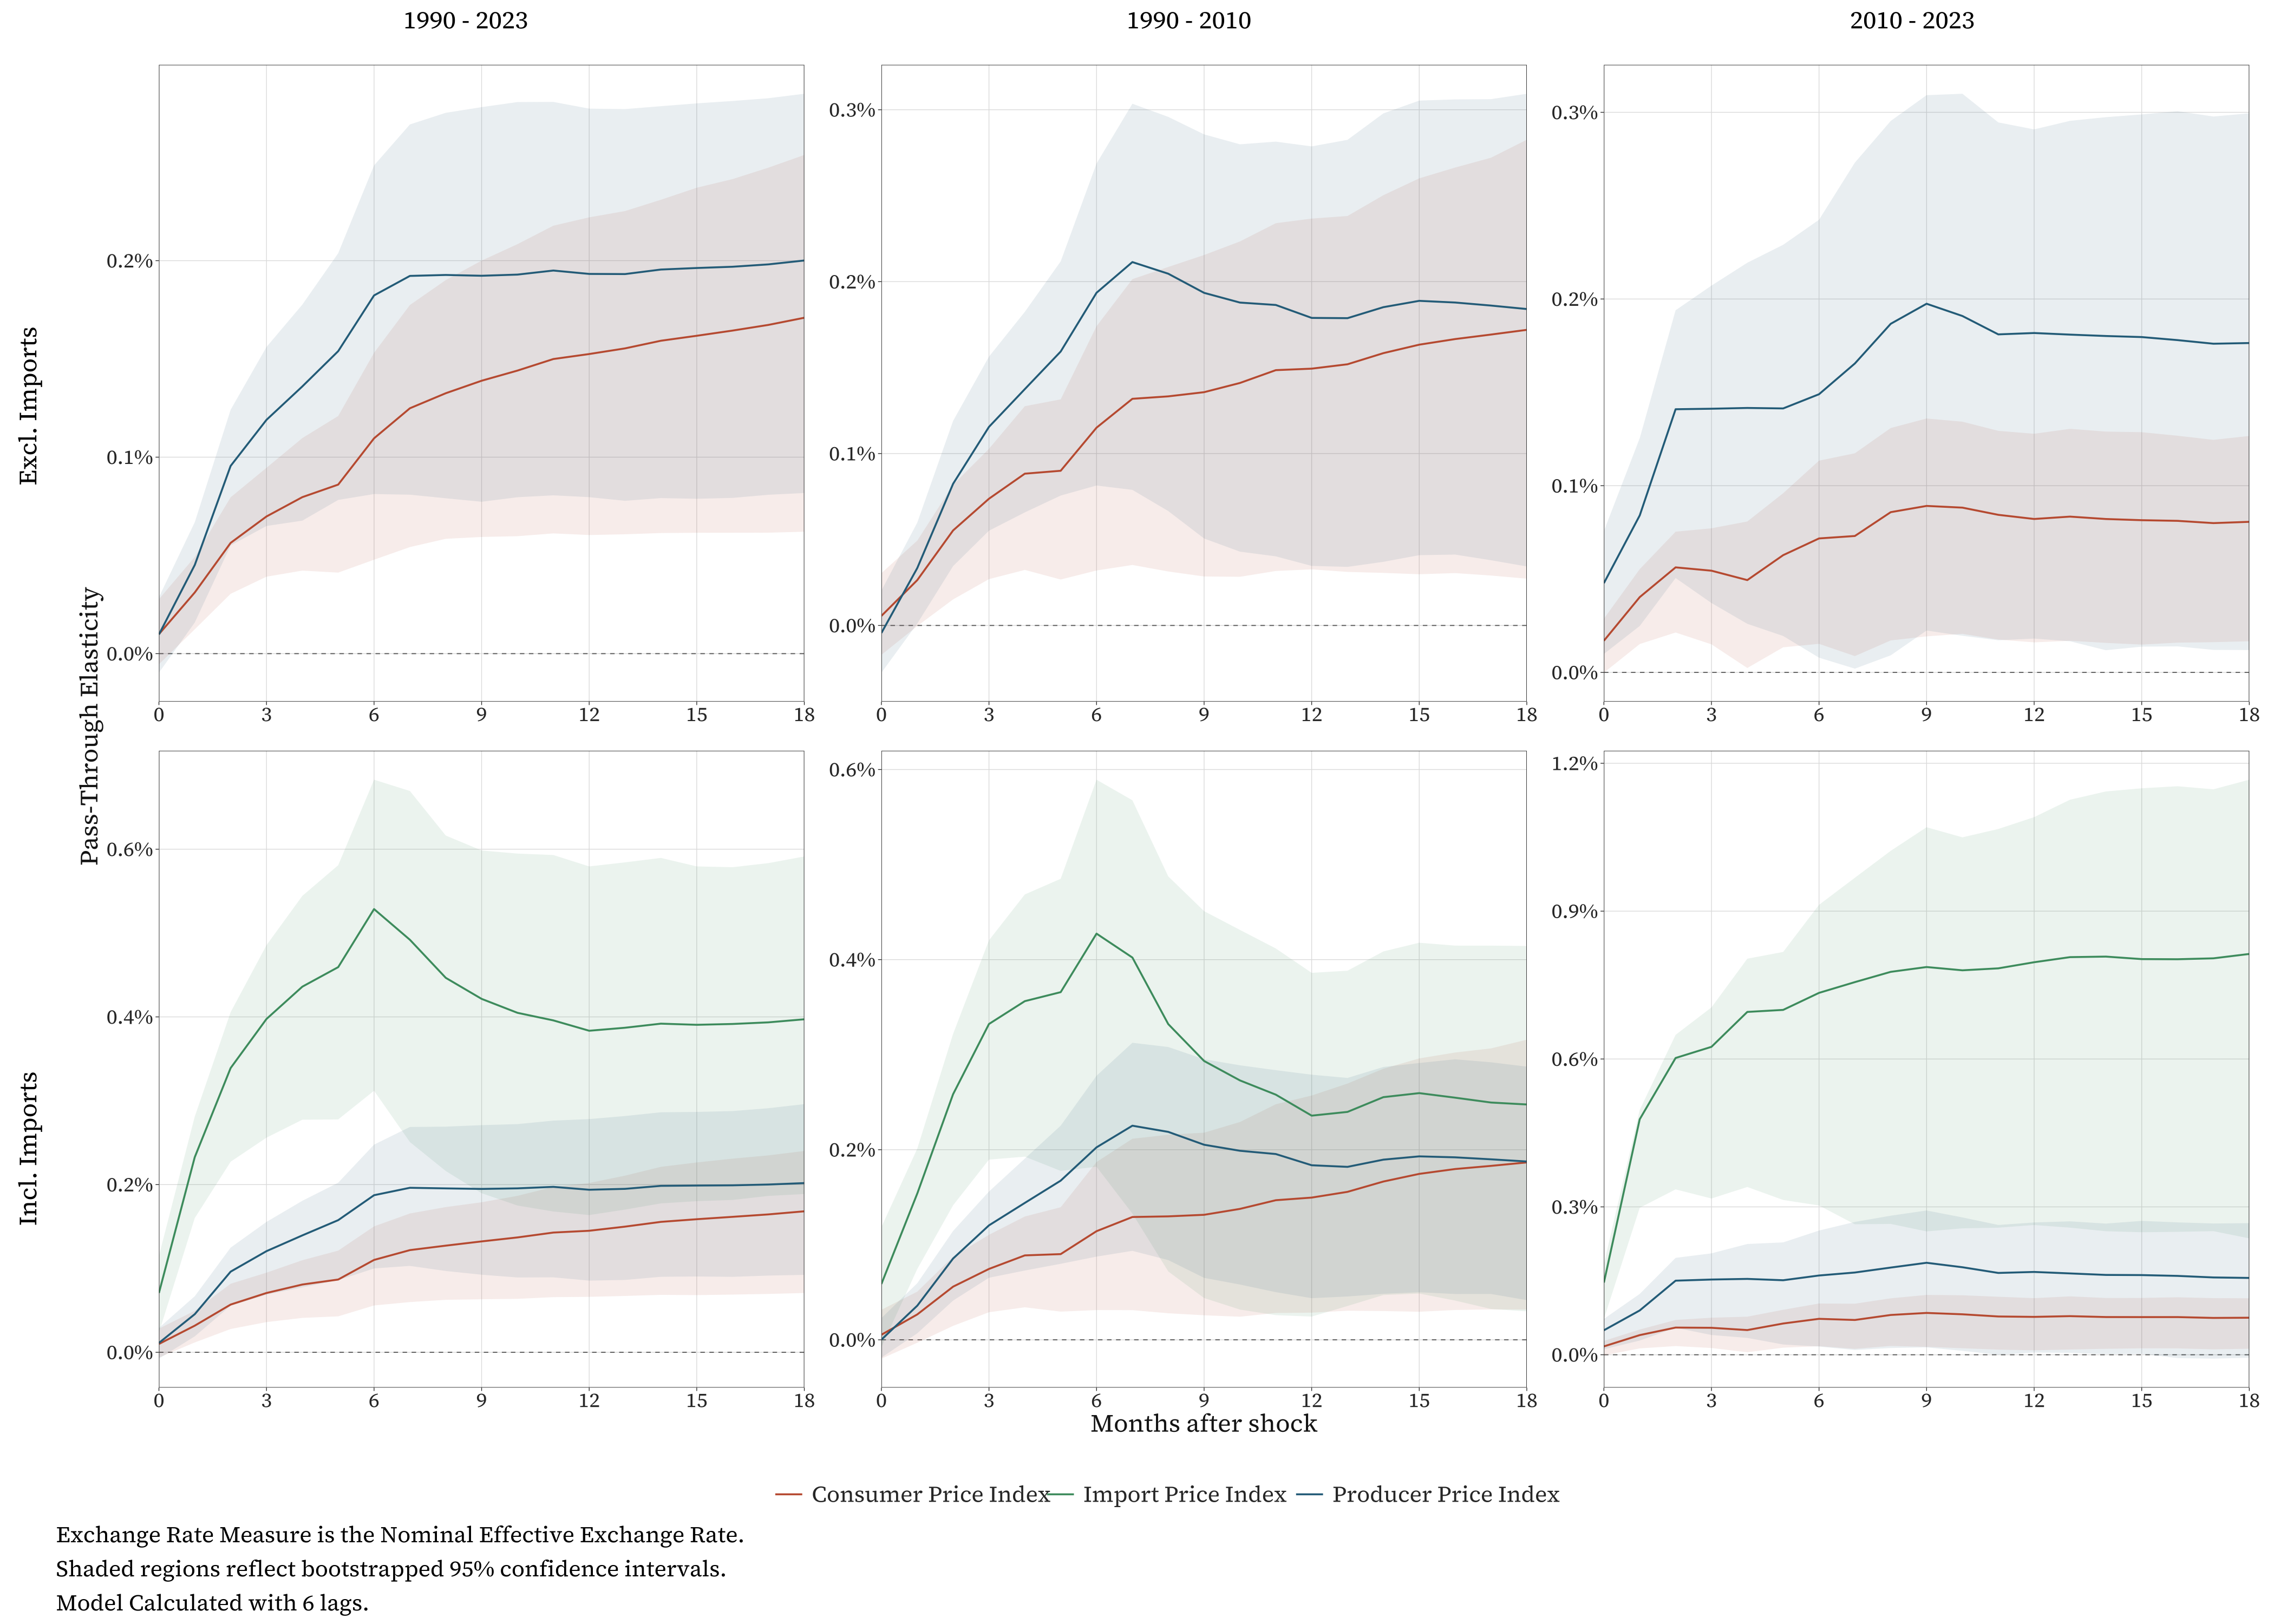
\includegraphics[width=\textwidth]{irf_main.png}
    \caption{Impulse Response Function Plots}
    \label{fig:irf_main}
\end{figure}

Figure \ref{fig:irf_main} provides a visual illustration of exchange rate pass-through to prices. \ref{erpt_main } in the Appendix shows exact values and bootstrapped standard deviations at select time horizons. The top row of Figure \ref{fig:irf_main} shows the result when only the latter 2 price indices are included. Looking at the full sample, the pass-through of a 1 percentage point change to the exchange rate to PPI after one quarter (3 months) is 0.12 percentage points, while after a year the total effect on producer prices is a 0.19 percentage point increase, with marginal changes over the rest of the horizon. In the same specification, CPI responds with a 0.07 percentage point increase after a quarter, increasing to 0.16 after a year, with little change seen after this. Over the two samples with different inflationary environments, there was little difference in the response of producers to changes in the exchange rate, with a 0.18 percentage point response in PPI after a year reported in both samples. For consumer prices, there seems to be a greater effect of inflationary environment on the responsiveness of prices. After a quarter, CPI had responded slightly more to exchange rate shocks in the early sample than when inflation was stable (0.07 compared to 0.05. The disparity seems to widen after a year: for the early sample it is estimated that consumer prices would be 0.15 pp higher after a percentage point depreciation of the Rand, while in the more recent period, it would have translated to just a 0.08 pp increase. The difference in the pass-through after a year for the two samples is considerable, with the estimate nearly halving from the high-inflation to the low-inflation sample. Despite this, a z-test for the difference in means using the bootstrapped standard errors\footnote{Calculated by $z = \frac{\hat{\psi}_1 - \hat{\psi}_2}{\sqrt{\hat{\sigma}_1^2 + \hat{\sigma}_2^2}}$} gives a p-value of 0.16, meaning findings are not statistically significant at conventional levels. 


The second row of panels in figure \ref{fig:irf_main}, import prices are included in the VAR model. Between 1990 and 2023, the pass-through of a 1 pp change in the exchange rate to import prices was 0.4 after a quarter and roughly the same after a year, although the interceding horizons do see spikes in the pass-through. Separating the full sample into the unanchored and stable inflationary periods, it is clear that the full sample estimates belie a great deal of intra-sample heterogeneity. While the effect of low inflation should lead to a lower pass-through estimate according to previous literature, the opposite is found to be the case, with initial pass-through two to three times as high over the first 12 months in the low inflation environment. Importantly, it does not follow from finding  that there was an increase in producer currency pricing relative to the less stable inflation period between 1990 and 2023, as the difference may be driven by the different measures of import prices used across the two periods. This highlights to a limitation in the fully-specified model, as intertemporal comparisons (ie comparing 1990 - 2010 to 2010 - 2023 estimates) may reflect differences in the way import price changes are measured. For this purpose, the model which excludes import prices is preferred. Nevertheless, estimates can still be useful to compare findings with other papers and to analyse pass-through along the pricing distribution. 

The early sample's estimate for pass-through is a lot lower than the single-equation estimates of \textcite{Karoroetal2008} and \textcite{kabundi2016exchange}, both of which estimating import PT to be above 0.75, while estimates by \textcite{aronetal2012} using a variety of specifications show PT after a year to be between 0.33 and 0.46 between 1995 and 2009. Although this places the 1990 - 2010 estimates at the lower end of estimates in South African studies, the 3-month PT of 0.33 is very close to the 0.31 reported for South Africa by \textcite{choudhri2015exchange}, which uses a similar model over the period from 1979-2010. The shape of the import price response curve also seems to differ significantly between the samples, with the early sample showing a reversal in pass-through after six months. This hump-shape was also reported in other studies of import prices by \textcite{mccarthy1999}, \textcite{hahn2003} and \textcite{AnWang2011}, however there is no evidence of a reversal in the 2010 - 2023 sample. Again, the series break complicates the investigation as it is not possible to discern whether this difference is due to changes in the way import prices are measured or whether there was less cost-switching after 2010. 

Across the three samples, there is consistent evidence of decreasing pass-through from importers price indices to PPI, followed by CPI. In the early sample, importers absorb 25\% of a 1\% change in the exchange rate over the course of a year,while for producers and consumers, the absorption is 19\% and 15\% respectively. While the discrepancy between importers and the latter two PT's is even greater in the low-inflation period, this is not necessarily evidence that would confirm the hypothesis that lower inflation leads to lower pass-through from import prices to consumer prices as the differences in measuring importers price changes across the samples may be driving this difference.

 There is some evidence of decreased pass-through from producers to consumers in the model which excludes import prices. Dividing consumer price PT by producer PT, it is found that after 3 months in the early sample, the PT in consumer prices was just under 70\% of that of producer prices, while after a year it was around 83\%. In the low inflation period,  PT to consumer prices is a third of producer prices PT after 3 months, rising to around 44\% after one year. Although this depends on the assumption that the omitted variable bias when excluding importers prices is of a similar magnitude and direction for producer and consumer prices, it does provide conditional evidence of the argument made by \textcite{taylor2000low} that producers are willing to absorb more of the increases in costs (due to higher import prices) when the cost increases are believed to be transitory. Some optimistic conclusion would be that the decrease in pass-through to consumer prices indicates that the country is now less dependent on imported consumer goods than in the early period, which would translate into a more muted effect of higher imported on overall consumer prices. A cursory look at South Africa's import-to-GDP ratio, however, shows the share of imported goods in the economy was higher during the previous decade than the preceding 20 years.
 
 Alternatively, a reasons for the dampened effect on consumer prices could be that increased competition among firms has increased the elasticity of demand facing firms and producers, meaning they cannot pass on cost increases as completely as before, as firms price to market. Another explanation - particularly plausible in the context of South Africa where electricity, transport and related infrastructure problems have become pertinent issues facing firms - is that distribution and other local costs have increased, making up a greater share of the total costs, leading to imported goods' prices having less of an impact of the prices of final goods, as suggested by \textcite{burstein2003distribution} and \textcite{goldberg2010sensitivity}. 
 
 Another difference between the samples visible from the impulse responses, is between the adjustment speeds, which are calculated as the PT at a particular horizon as a percentage of the PT after a year - the point when PT seems to settle at a particular value\footnote{\textcite{hahn2003} and \textcite{comunale2017erpt} employ a similar technique, using different horizons as their settled point.}, seen in Figure \ref{fig:adj_main}.  While prices were found to respond sequentially in the early sample, with import prices reaching the 12-month pass-through level within 3 months (although it continues to rise significantly before settling at 12 months), PPI PT rising to its maximum in 6 and consumer prices after a year. This is consistent with \textcite{clark1999responses}'s findings around the sequential response to monetary policy and other literature on ERPT. This is not observed in the new sample, with the panels in the third column showing prices to reach their respective pass-through levels at a similar pace. Given the higher degree of absolute pass-through seen for import prices, it should be noted that a 50\% adjustment for import prices would result in far greater price changes than a 50\% change in the other two given how much higher the PT is for import prices. Looking back at Figure \ref{fig:irf_main}, the steepness of the import impulse response over the first 3 months does indicate it is relatively more responsive than is suggested by the adjustment speed plot. 
 
\begin{figure}[H]
    \centering
    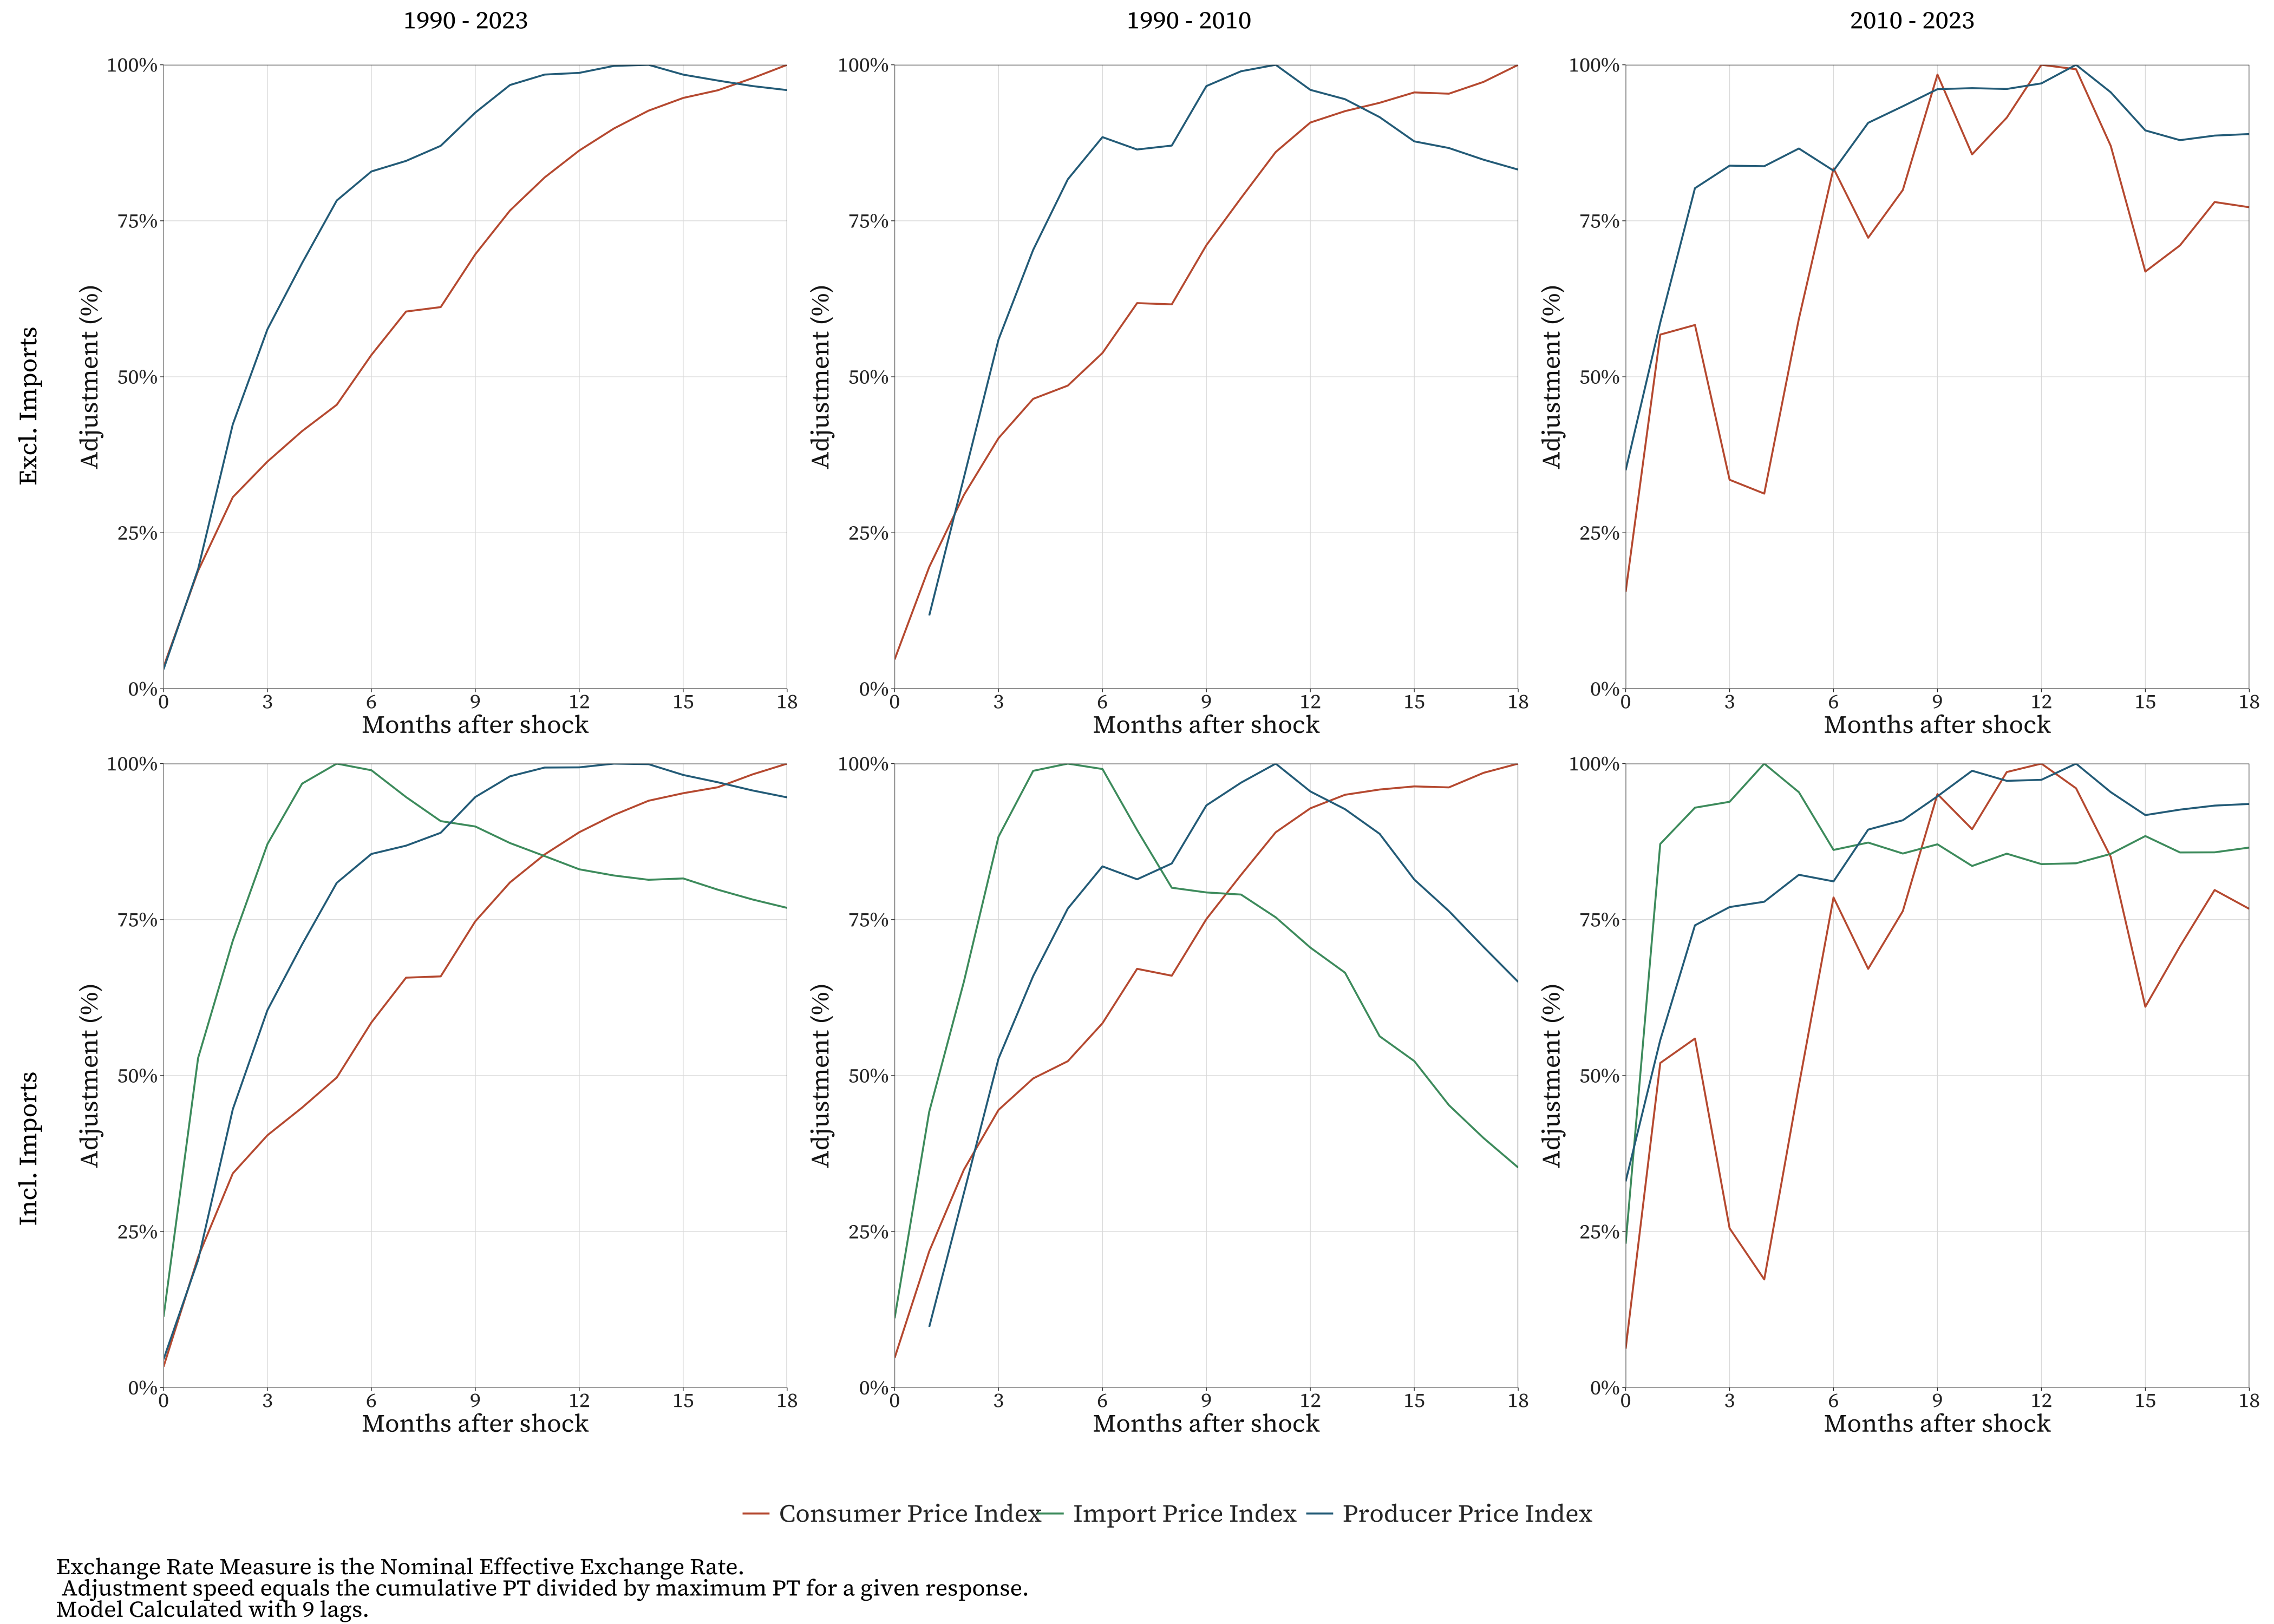
\includegraphics[width=\textwidth]{adj_main.png}
    \caption{Adjustment Speed Plots}
    \label{fig:adj_main}
\end{figure}

\subsection{Variance Decompositions}

Another way of assessing the importance of exchange rate movements in determining price movements is by variance decomposition. Across all of the specifications and samples, there is a clear decline in the role of exchange rates in determining prices as one moves from import prices to consumer prices. In the full sample, the proportion of import price variance attributable to exchange rate movements was 0.23 after 3 months and nearly a quarter after a year. Again, this figure masks strong differences between the early and later samples, with the early sample suggesting around a fifth of import price variance attributable to exchange rate shocks, while the post-2010 shows half of the variance in import prices to stem from exchange rate shocks in the first 3 months, settling at around 43\% after a year. 

With the latter two prices, the contribution to CPI variance is slightly lower than for PPI variance across all samples and specifications, consistent with the idea that downstream noise resulting from distribution and other domestic costs dilutes the overall contribution of exchange rate shocks.  Additionally, the differences between the 1990 - 2010 and 2010 - 2023 samples are far less pronounced than the differences in the import prices across the two periods: after a year, the fully specified model shows exchange rate shocks to have accounted 13.4\% of the variation seen in PPI in the early sample and 15.8\% in the low-inflation period - a difference of around 2\%. For CPI, the difference is around 3\%. This indicates that the contribution of exchange rate shocks relative to other shocks in explaining PPI and CPI has remained relatively stable across the two periods. 

\input{main_fevd.txt}

\subsection{Historical Decomposition}

To see how orthogonal exchange rate shocks have materially affected inflation in South Africa since 1990, historical decompositions are plotted in Figure \ref{fig:hist_main} to demonstrate the disturbance to prices caused by exchange rate movements. Over the course of the 33 years in the sample, there are large positive spikes at a number of dates, particularly in early 2002 and 2008 as well as 2016. Each of these coincided with major economic and political developments which saw  large depreciations in the Rand. The most dramatic of these - late 2001 to early 2002 -  saw the value of the Rand depreciate by over thirty percent, trading at R8.05 on the Dollar in June 2001 to R11.38 by March 2002, with the September 11 attacks and a series of crises in developing and middle-income countries likely contributing to risk-off investor sentiment \parencite{sarb2002qb, sarb2001qb}. In contrast to the earlier negative shock to the Rand, the spikes in 2008 and 2016 coincided with domestic affairs The former happened in the wake of two major events: the defeat of the market-friendly faction of the ruling African National Congress at the party's 2007  congress and the first power outages by the national electricity utility while the politically-motivated appointment of a new finance minister in December 2015, an event that became known as "Nenegate" after the ousted minister Nhlanhla Nene,  alerted investors to the increasing loss of institutional independence. Each of these events had varying degrees of independence from supply and demand shocks, thus representing relatively sizeable orthogonal disturbances to the exchange rate. Another large contribution is seen in July 2022, likely the result of  the the US Fed's interest hikes that began in 2022, which would have led to a risk-off move away from emerging markets and sizeable depreciations of the Rand relative to advanced economies. 

The differing relationship between exchange rate shocks and domestic prices before and after 2010 is seen in the reaction to these events. Using the 1990 - 2010 covariance structure, the crises of late 2001 contributed to an elevation of producer prices by about a percentage point and half a percentage point for consumer prices, while the major event of the late sample - Nenegate - raised producer prices by under half a percentage point and consumer prices by around a quarter. Although early 2016 actually saw around the same level of inflation as early 2002 at around 6\%, the lower contribution is not necessarily evidence of the decline in PT to consumer prices across the two periods as the difference in magnitude of the shocks could be driving the difference. Nevertheless, whether by a decrease in the volatility around the exchange rate or through a partial decoupling of the structural relationship between exchange rate and prices, historical plots show that the contribution to inflation by exchange rate events has decreased. 


 
\begin{figure}[H]
    \centering
    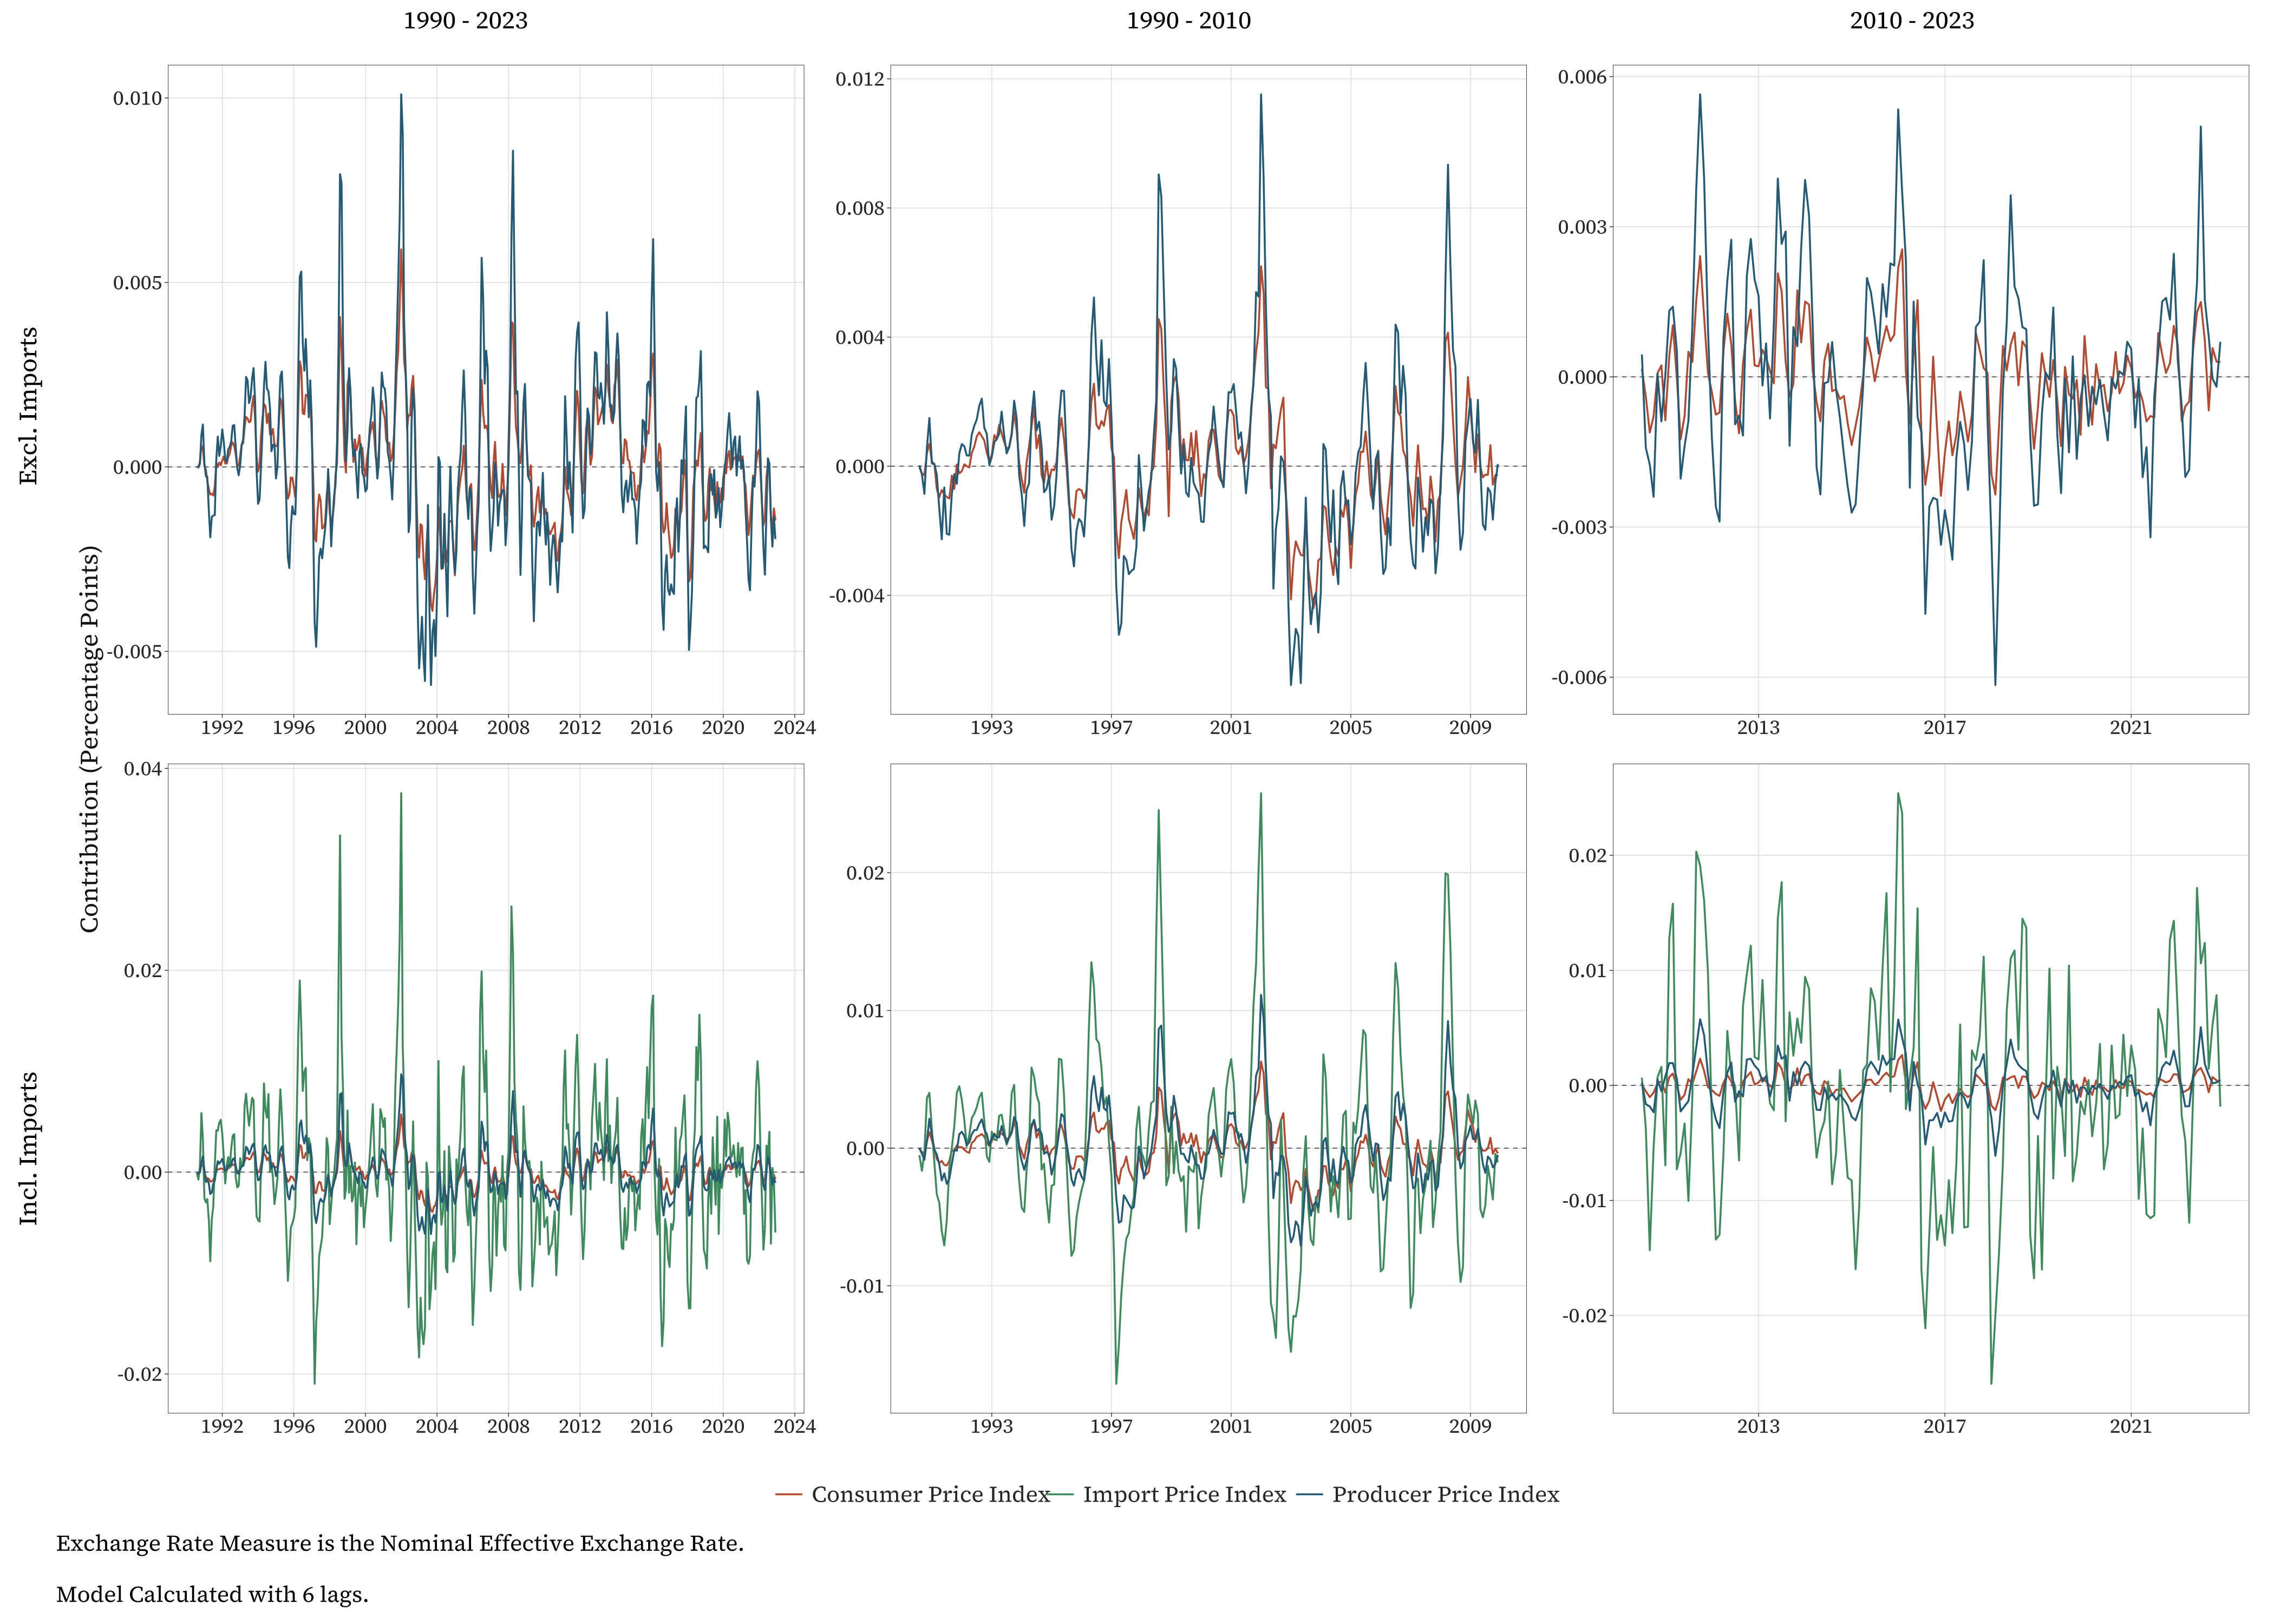
\includegraphics[width=\textwidth]{hist_main.png}
    \caption{Historical Contribution Plots}
    \label{fig:hist_main}
\end{figure}


\pagebreak

\section{Robustness Checks}

The preceding results established the degree of pass-through from exchange rate shocks into South African prices and showed evidence of the declining responsiveness to these shocks. Within the recursive identification strategy first used in \textcite{mccarthy1999}, there are several  variations, including the modifications made in the previous section - namely entering oil supply as an exogenous variable and omitting the import price index. While there was little difference in PPI and CPI outcomes when import prices were omitted compared to when it was included, other specifications are explored in order to verify the robustness of the main results. Estimations using different lag lengths, endogenised oil supply, monetary policy and linear projections are analysed in turn. 

\subsection{Lag Length}

  The tendency of AIC to pick out more parsimonious models with shorter lag lengths risks longer-horizon dynamics being omitted. Oil shocks, for example, can have gradual or delayed impacts on economic variables, meaning that short lag lengths may miss these effects altogether \parencite{EDELSTEIN2009766, hamilton-herrera}. The possibility that these longer-term relationships may materially influence results are explored by running models using both 9 and 12 lags - the latter equal to the numbers chosen by \textcite{mccarthy1999} and \textcite{hahn2003}. Figure \ref{fig:irf_p9} and Table \ref{tab:erpy_p9} in Appendix A2 show the impulse responses and forecast error variance from 9 and 12 lags. Results from the 9-lag model are nearly identical across all samples and both specifications. Including 12 lags, the model estimates similar values for the first 12 months, however PT estimates do not converge and either continue to increase or fall over longer horizons. It is evident, particularly in the short sample, that extending the lags has considerable effects on the certainty of the estimates, with standard errors increasing particularly at longer horizons as more noise enters the model. Nevertheless, the in estimates across different lag lengths do not differ much over the first 12 months. 

\subsection{Endogenous Oil Shocks}

The exogeneous K\"anzig oil supply series is preferred as a better proxy for global supply conditions than crude spot prices, which may be a reflection of demand pressures in addition to supply conditions. Moreover, as a small economy, South Africa's domestic activity is unlikely to have any material effect on oil supply. Including oil supply in the endogenous system therefore risks distorting oil shocks due to spurious correlation with other variables in the system. Previous literature, however, typically predates the availability of oil supply series and have studied OECD countries which are more likely to have some impact on oil markets. These have typically opted to use Brent Crude spot prices entered endogenously. Entering the \cite{imf_pcps} Brent Crude spot price as was done by, among others, \textcite{mccarthy1999} and \textcite{AnWang2011}, there is little difference in our estimates evident in Appendix A3, with differences between corresponding estimates typically being 0.01 to 0.05\footnote{Note that the Brent Crude spot price index was only available from 1992, meaning the sample is shortened by 2 years.}. Table \ref{tab:fevd_oil} shows that the relative contribution of exchange rate shocks is similar regardless of how oil supply is entered into the model. 

\subsection{Monetary Policy}

Monetary policy and inflationary regimes form a key part of this study, however interest rates do not explicitly enter the main specification as placing it prior to the exchange rate would orthogonalise the exchange rate shocks with respect to interest rate movements would partially remove developments in risk premia and international financial market dynamics which drive the changes in exchange rates. It is also not immediately obvious where in the ordering it belongs with Cholesky decomposition. On one hand exchange rates are influenced by interest rate differentials, while on the other it may not be implausible to suggest that exchange rate innovations can have contemporaneous impacts on interest rates. Although omitted by \textcite{mccarthy1999}, it is included by \textcite{hahn2003} and \textcite{cazorzi2007}. The South African Real Prime Rate is entered into the equation between the output gap and the exchange rate variables. 

From the results in Appendix A4, the effect of adding interest rates into the equation seems only to influence PT estimates in the low-inflation sample. For imports, the 12-month PT is now around 0.93 compared with 0.8 in the previous sample. For PPI, the pass-through between 2010 and 2023 was marginally higher across the imports-inclusive and imports-exclusive models once interest rates are controlled for 0.21 compared with 0.17 and 0.22 as oppose to 0.18 when interest rates aren't included. Consumer prices in the low-inflation period are now 0.11 and 0.12 with and without import prices respectively, as oppose to 0.08 in both cases in our main specification. In both these cases, pass-through to consumer prices are still lower than in the more inflationary period. The addition of a fourth (in the import-free specification) and fifth (for the full specification) endogenous variable to the equation does come at the expense of some degrees of freedom, however the increase in the (bootstrapped) standard errors is not very large in most cases. 

As mentioned, the inclusion of the interest rate variable ahead of the exchange rate in the recursive ordering risks removing financial market innovations from the exchange rate movements given the role of risk premia and investor sentiment in determining both market interest rates and exchange rate movements. That the estimates for exchange rate movements which are orthogonal to interest rate movements do not differ from those which are not suggests that the contemporaneous correlation between interest rates and exchange rates is not substantial enough to materially impact the estimates.

\subsection{Linear Projections} 

VARs are typically used throughout previous literature, thus providing a well-established theoretical framework and results with which to compare findings. Through using a VAR model, dynamic interactions between variables can be more precisely estimated, however to the extent that the VAR dynamics diverge from reality, estimates may suffer from misspecification bias. To address this possibility, the main results from the SVAR are compared with results obtained from local projections as per \textcite{Jorda2005}. This is done in two stages: the first by regressing the exchange rate on oil and demand shocks in order to recover impulses and the second by regressing the price variables on  across horizon $h$ on the exchange rate disturbance along with a set of lagged controls. The upshot of this specification is that deviating from the structure imposed by the Cholesky ordering and allowing PPI and CPI to respond freely enables verification of the recursive structuring: if the LP response profile of the prices is found to resemble that of the VAR responses, there is evidence of a pricing distribution chain in the data. 

Table \ref{tab:erpt_lp} in Appendix A5  shows the ERPT elasticities from the linear projections. There is some evidence that the Cholesky ordering of the prices is correct: Across each of the horizons in the first 12 months, there is very little difference in the PT elasticity estimates. Indeed, a look at Figure \ref{fig:irf_lp} (Also Appendix A5) shows that the shapes are very similar to those of the baseline plots for the first 12 months, after which point the Newey-West standard errors and confidence intervals expand dramatically. Figure \ref{fig:lp_adj_plots} provides support for the ordering in our VAR model, with plots very similar to those in Figure \ref{fig:adj_main} as producer prices seem to react relative quicker than consumer prices across both samples even without the ordering restriction, while import prices react most immediately in the early sample. Again, the magnitude of the import price response in the low inflation sample means that the adjustment plot is somewhat deceiving given how large a 70\% adjustment in import prices is relative to producer prices due to the magnitude of the import price response in the new sample. 

The similarity over short to medium horizons relative to $p$ followed by the divergence at longer horizons is consistent with the comparisons made between VAR and LP's by \textcite{montielolea2025lp}, who showed that the difference in model standard errors expand at longer horizons. This also reflects the bias-variance trade-off that characterises the differences between the models: whereas VAR models yield tighter confidence intervals, this certainty is the results of structural assumptions embedded in the recursive identification, thus dependent on the accuracy of these assumptions. 

\pagebreak

\section{Conclusion}

The SARB operates under a singular mandate of ensuring the value of the Rand is maintained. This is complicated by, among other structural features of the South African economy, the high degree of responsiveness of the Rand to external shocks. The extent to which exchange rates are felt by consumers is reflected in the elasticity of the exchange rate pass-through estimate. On one hand, the rise in the share of imported goods may have led to an increase in the degree of pass-through, while on the other, a more stable price environment may have reduced this. The preceding findings of this paper offer some support that the effect of price stability since the 2010's has helped reduce the magnitude of pass-through. With estimates for 12-month PT of  0.08 in the low inflation sample and 0.14 in the full sample, South Africa shows low levels of pass-through relative to other emerging economies according to the findings of \textcite{cazorzi2007} and comparable to those of advanced economies. 

Although the evidence cannot be confirmed at statistical significances, this is supportive of theory and evidence from past literature. \textcite{taylor2000} hypothesised that if firms view cost shocks as transitory, consistent with low-inflation environments, they are more willing to accept short-term fluctuations in their profits. Among studies that support this are \textcite{gagnon2004monetary}, \textcite{schultz2007} and textcite{ozkan2015time}. In the context of South Africa specifically, this study's evidence corroborates the findings of \textcite{jooste2014determinants}, who show inflation variability to influence pass-through to consumer prices. 

The support given to the connection between inflation and pass-through adds an additional basis for the importance of retaining price stability: by keeping inflation low, import price shocks are not passed through to consumers as much as they would be if costs are expected to continue to rise. Various headwinds remain for price stability: global oil crises, domestic and international political uncertainty, and financial cycles can all have dramatic impacts on investor sentiments towards South Africa, which could lead to large shocks to the exchange rate. Should these coincide with higher inflation rates, the challenges would be compounded by firms passing on exchange rate shocks if they view these to be more persistent. Thus resulting in a double jeopardy whereby large shocks have higher pass-through. 

This paper has provided some evidence of recent developments in ERPT in South Africa, however there remain several shortcomings and unanswered questions that can be addressed by future research. The most obvious of these would be through the recovery of an updated and continuous series for import price indices. Its absence has imposed limitations on the ability of this study to look at the responsiveness over time and forced a shorter sample. In order to identify the factors that determine pass-through, alternative specifications would be necessary. Another possible endeavour would be to analyse the disaggregated responses across different categories of goods. Unfortunately, these series are also characterised by discontinuities. Finally, while a simple but well-motivated discrete break was used to recover differences in pass-through across inflationa regimes, a smooth-transition VAR model provides a way to measure continuous changes in the exchange rate pass-through as the inflationary environment switches. 

\pagebreak
\printbibliography
\pagebreak

\section{Appendix}

\subsection*{Appendix A - Results}

\input{main_results.txt}


\subsubsection*{A2 - Lag Selection}

\begin{figure}[H]
    \centering
    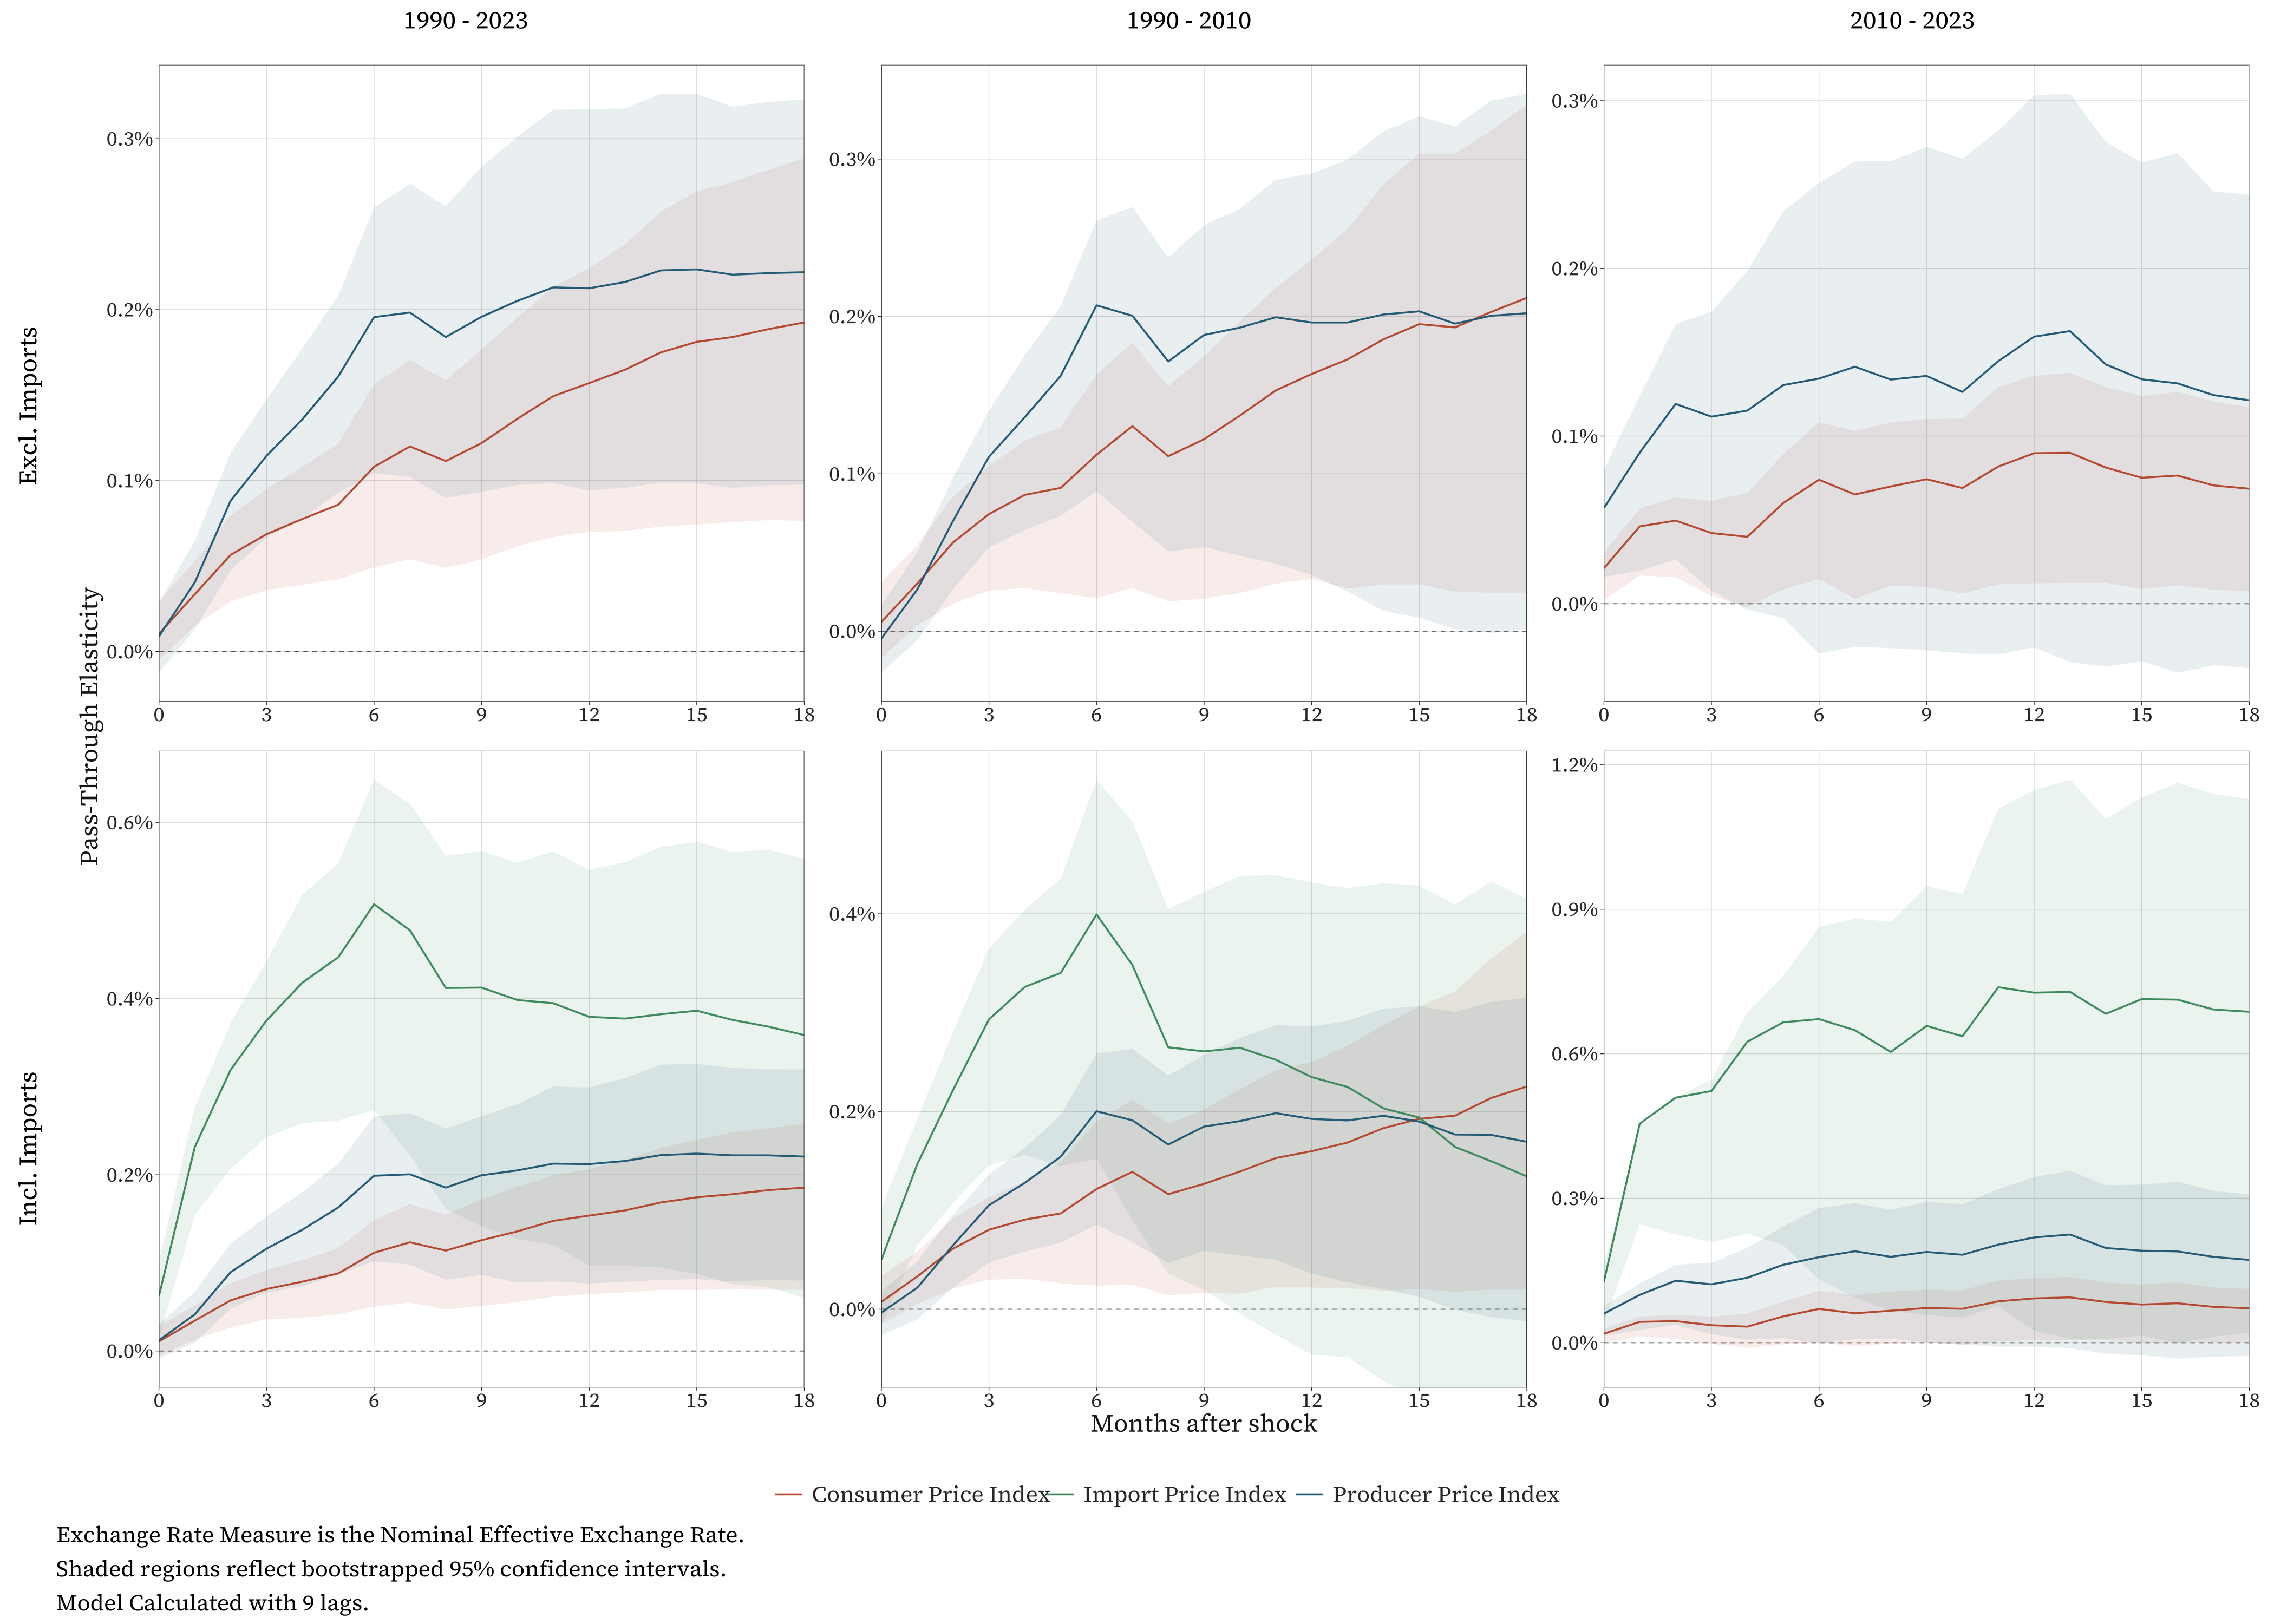
\includegraphics[width=\textwidth]{irf_p9.png}
    \caption{Impulse Response Functions with 9 Lags}
    \label{fig:irf_p9}
\end{figure}

\input{p9_results.txt}

\begin{figure}[H]
    \centering
    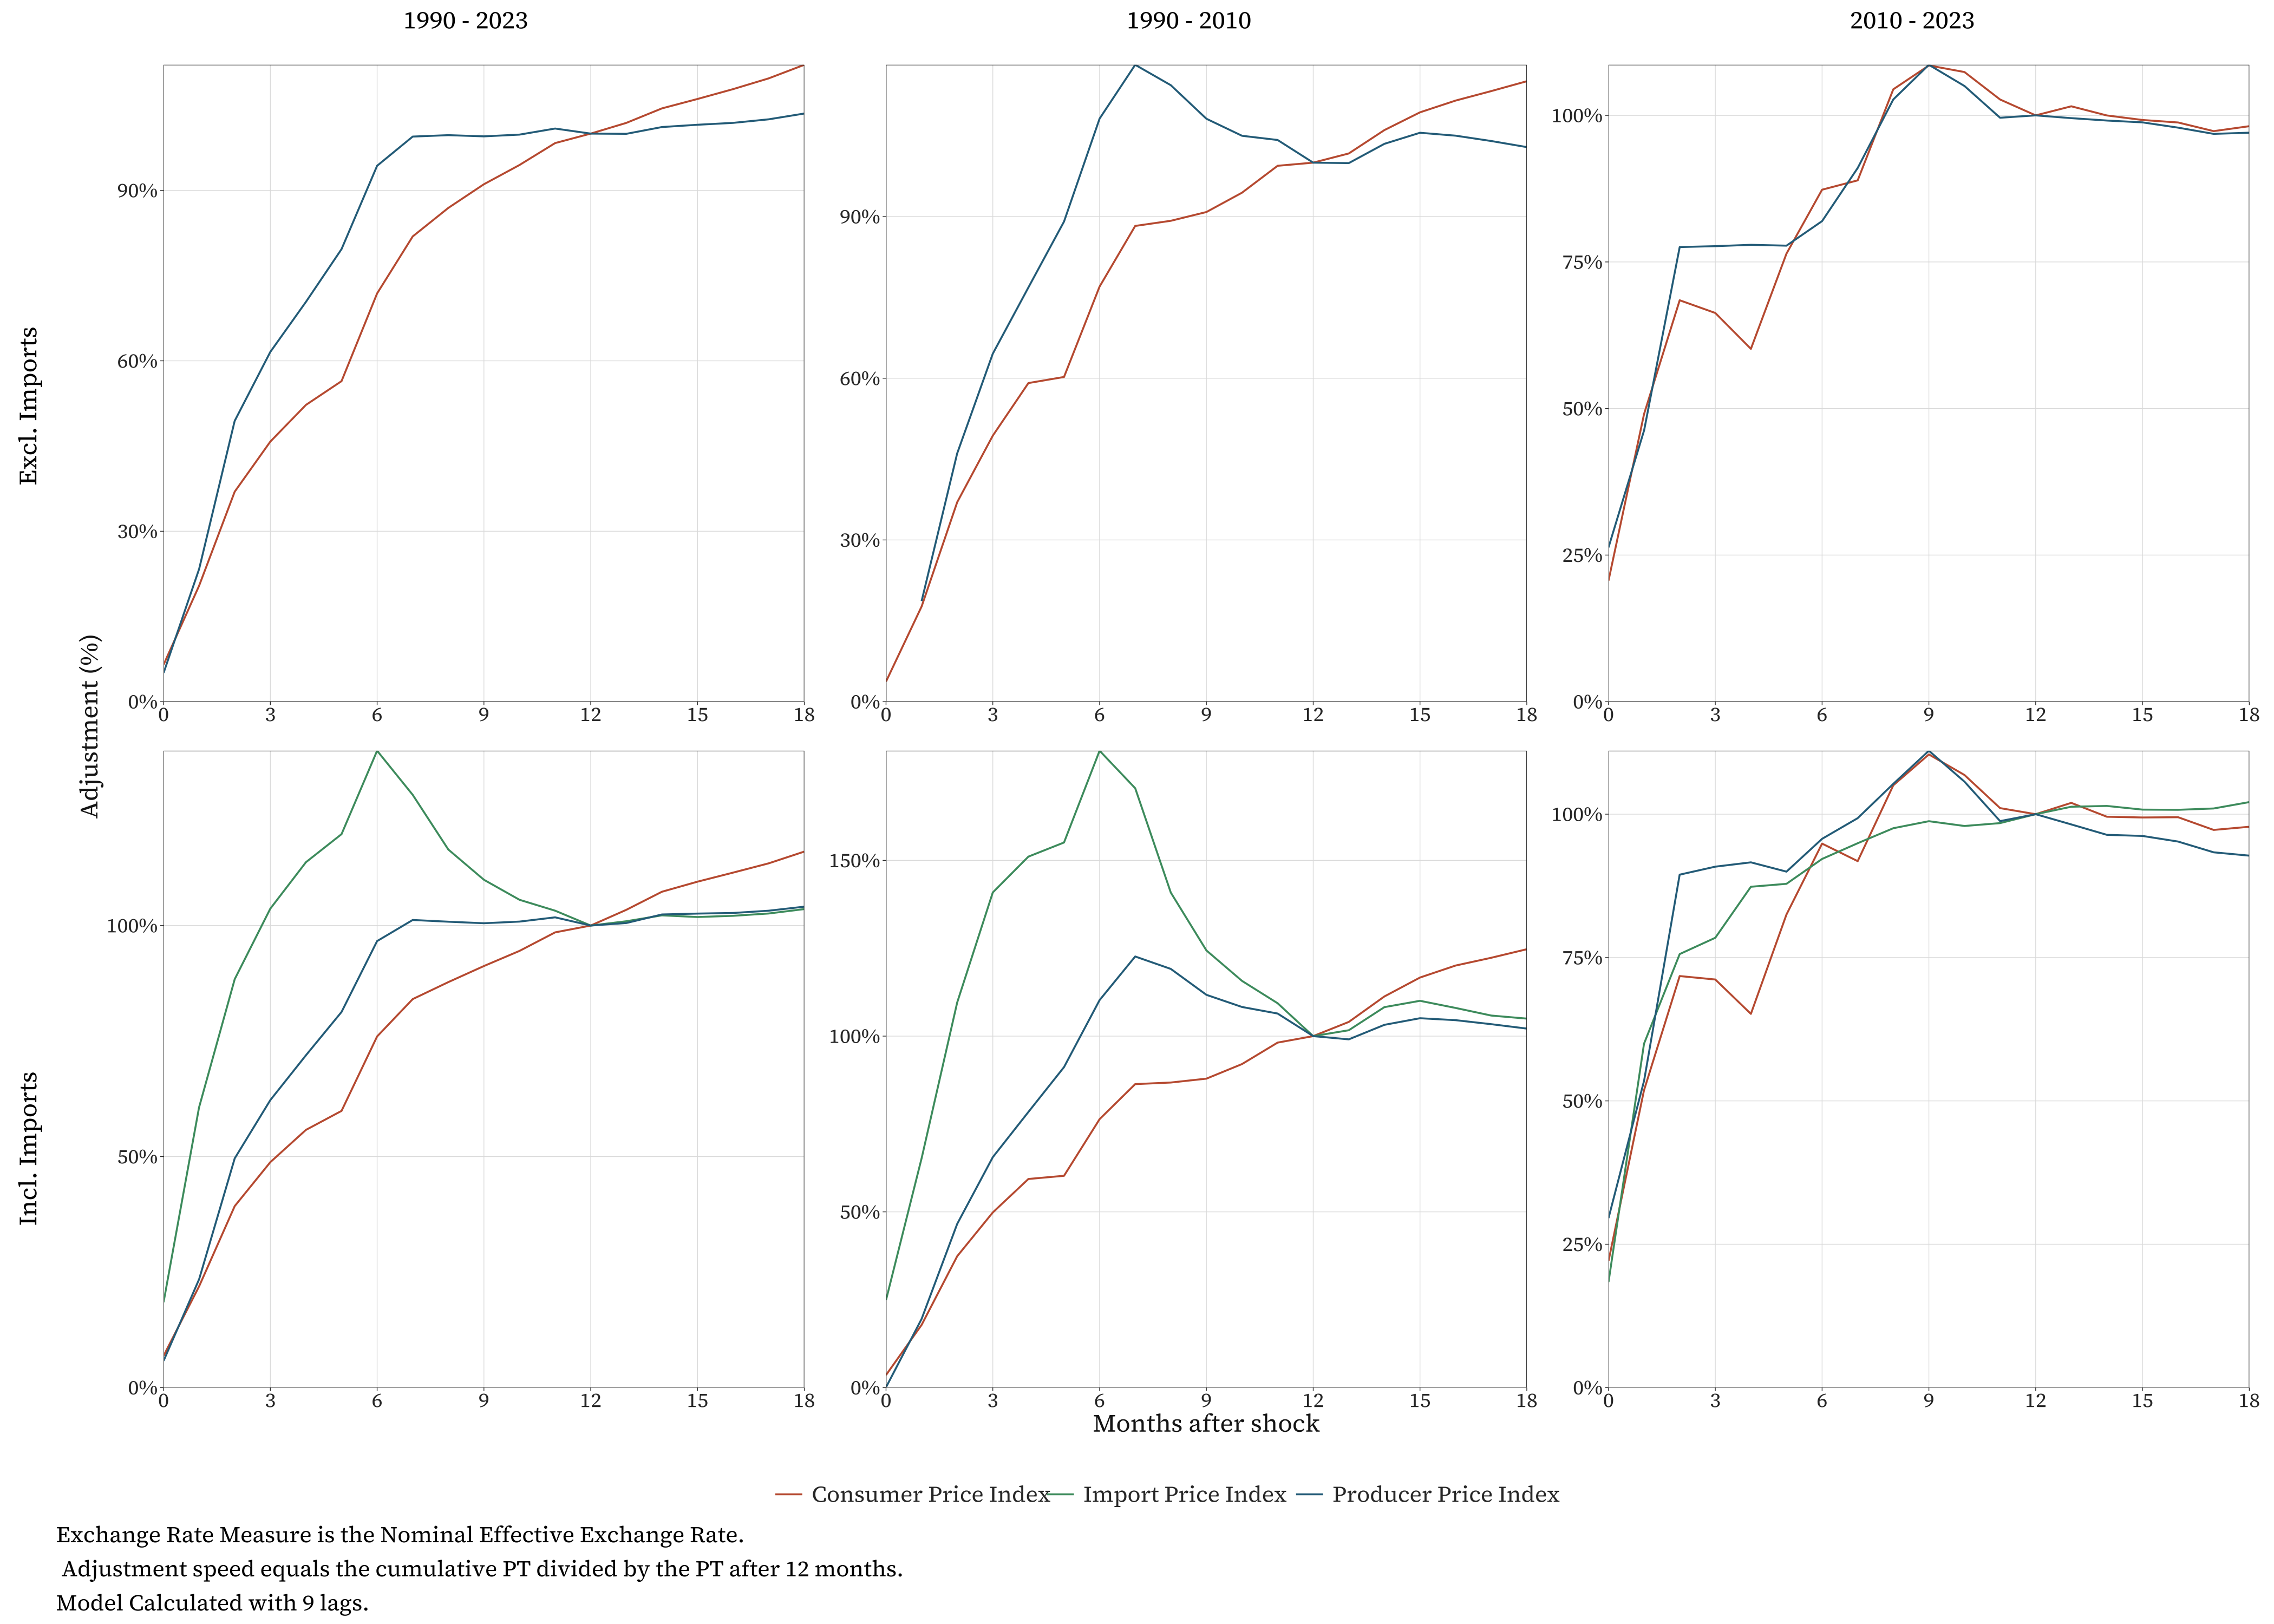
\includegraphics[width=\textwidth]{adj_p9.png}
    \caption{Adjustment Speed Plots with 9 Lags}
    \label{fig:p9_adj_plots}
\end{figure}

\input{p9_fevd.txt}


\begin{figure}[H]
    \centering
    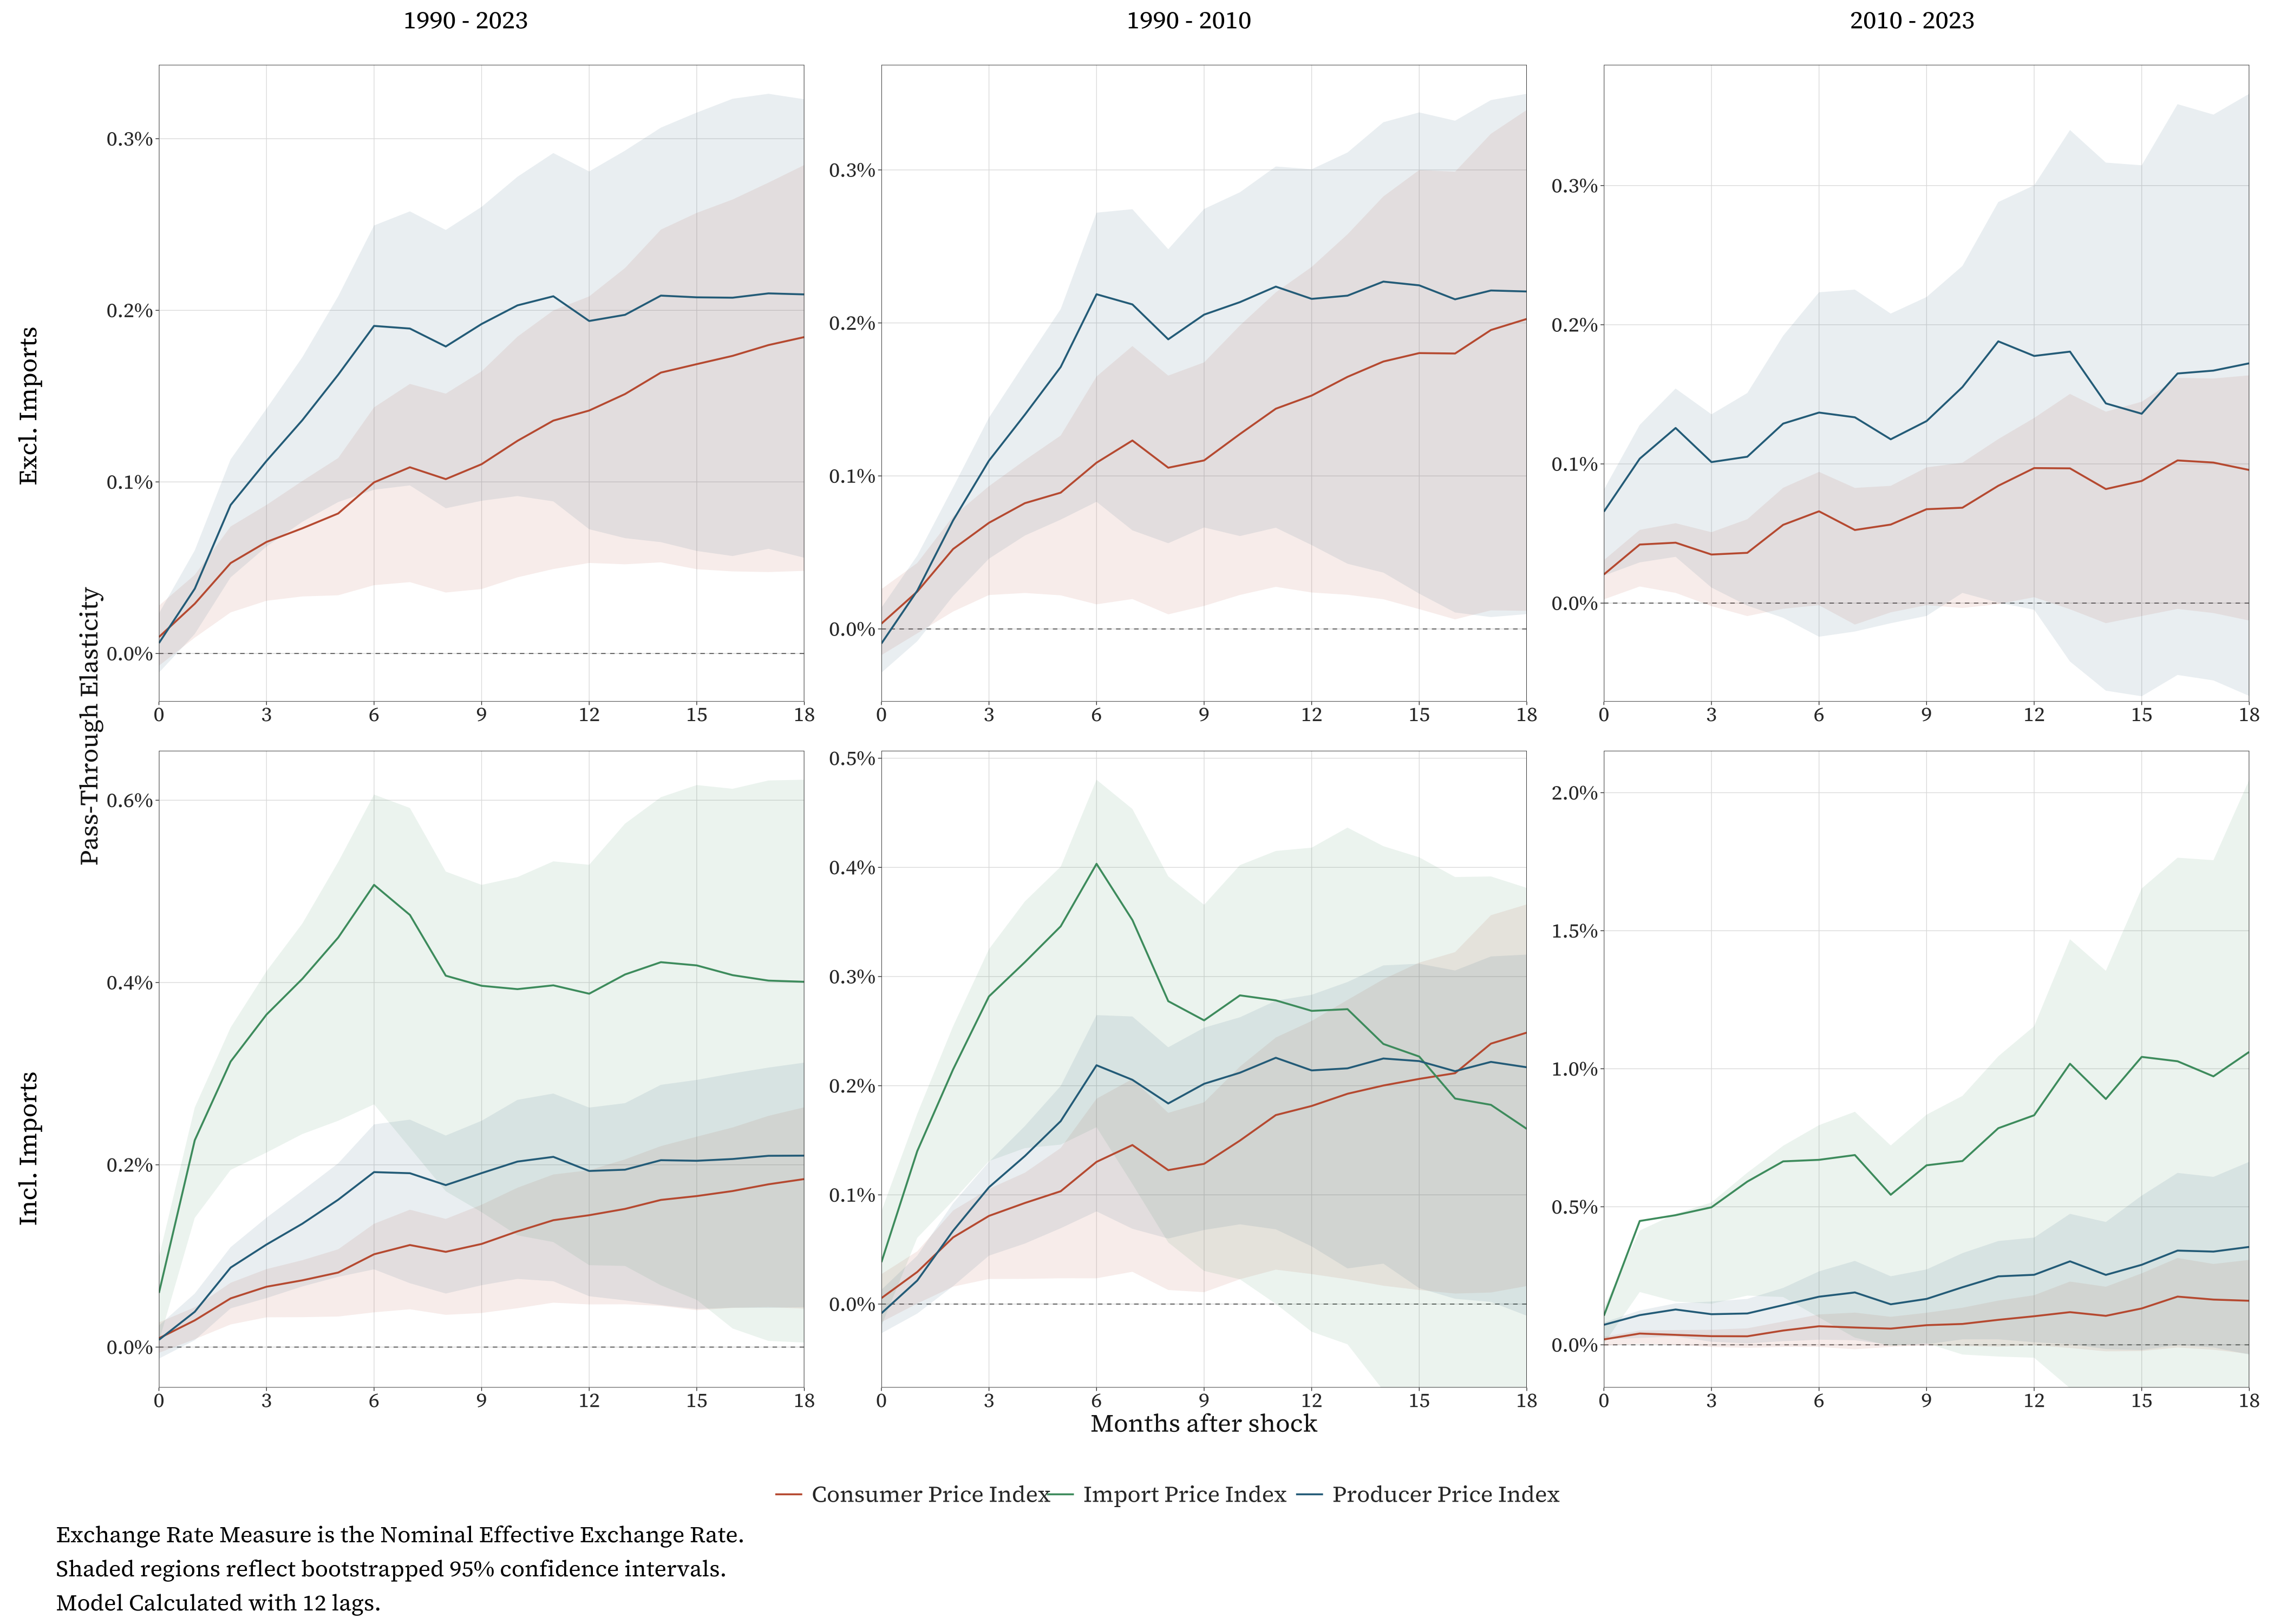
\includegraphics[width=\textwidth]{irf_p12.png}
    \caption{Impulse Response Functions with 12 Lags}
    \label{fig:irf_p12}
\end{figure}

\input{p12_results.txt}


\begin{figure}[H]
    \centering
    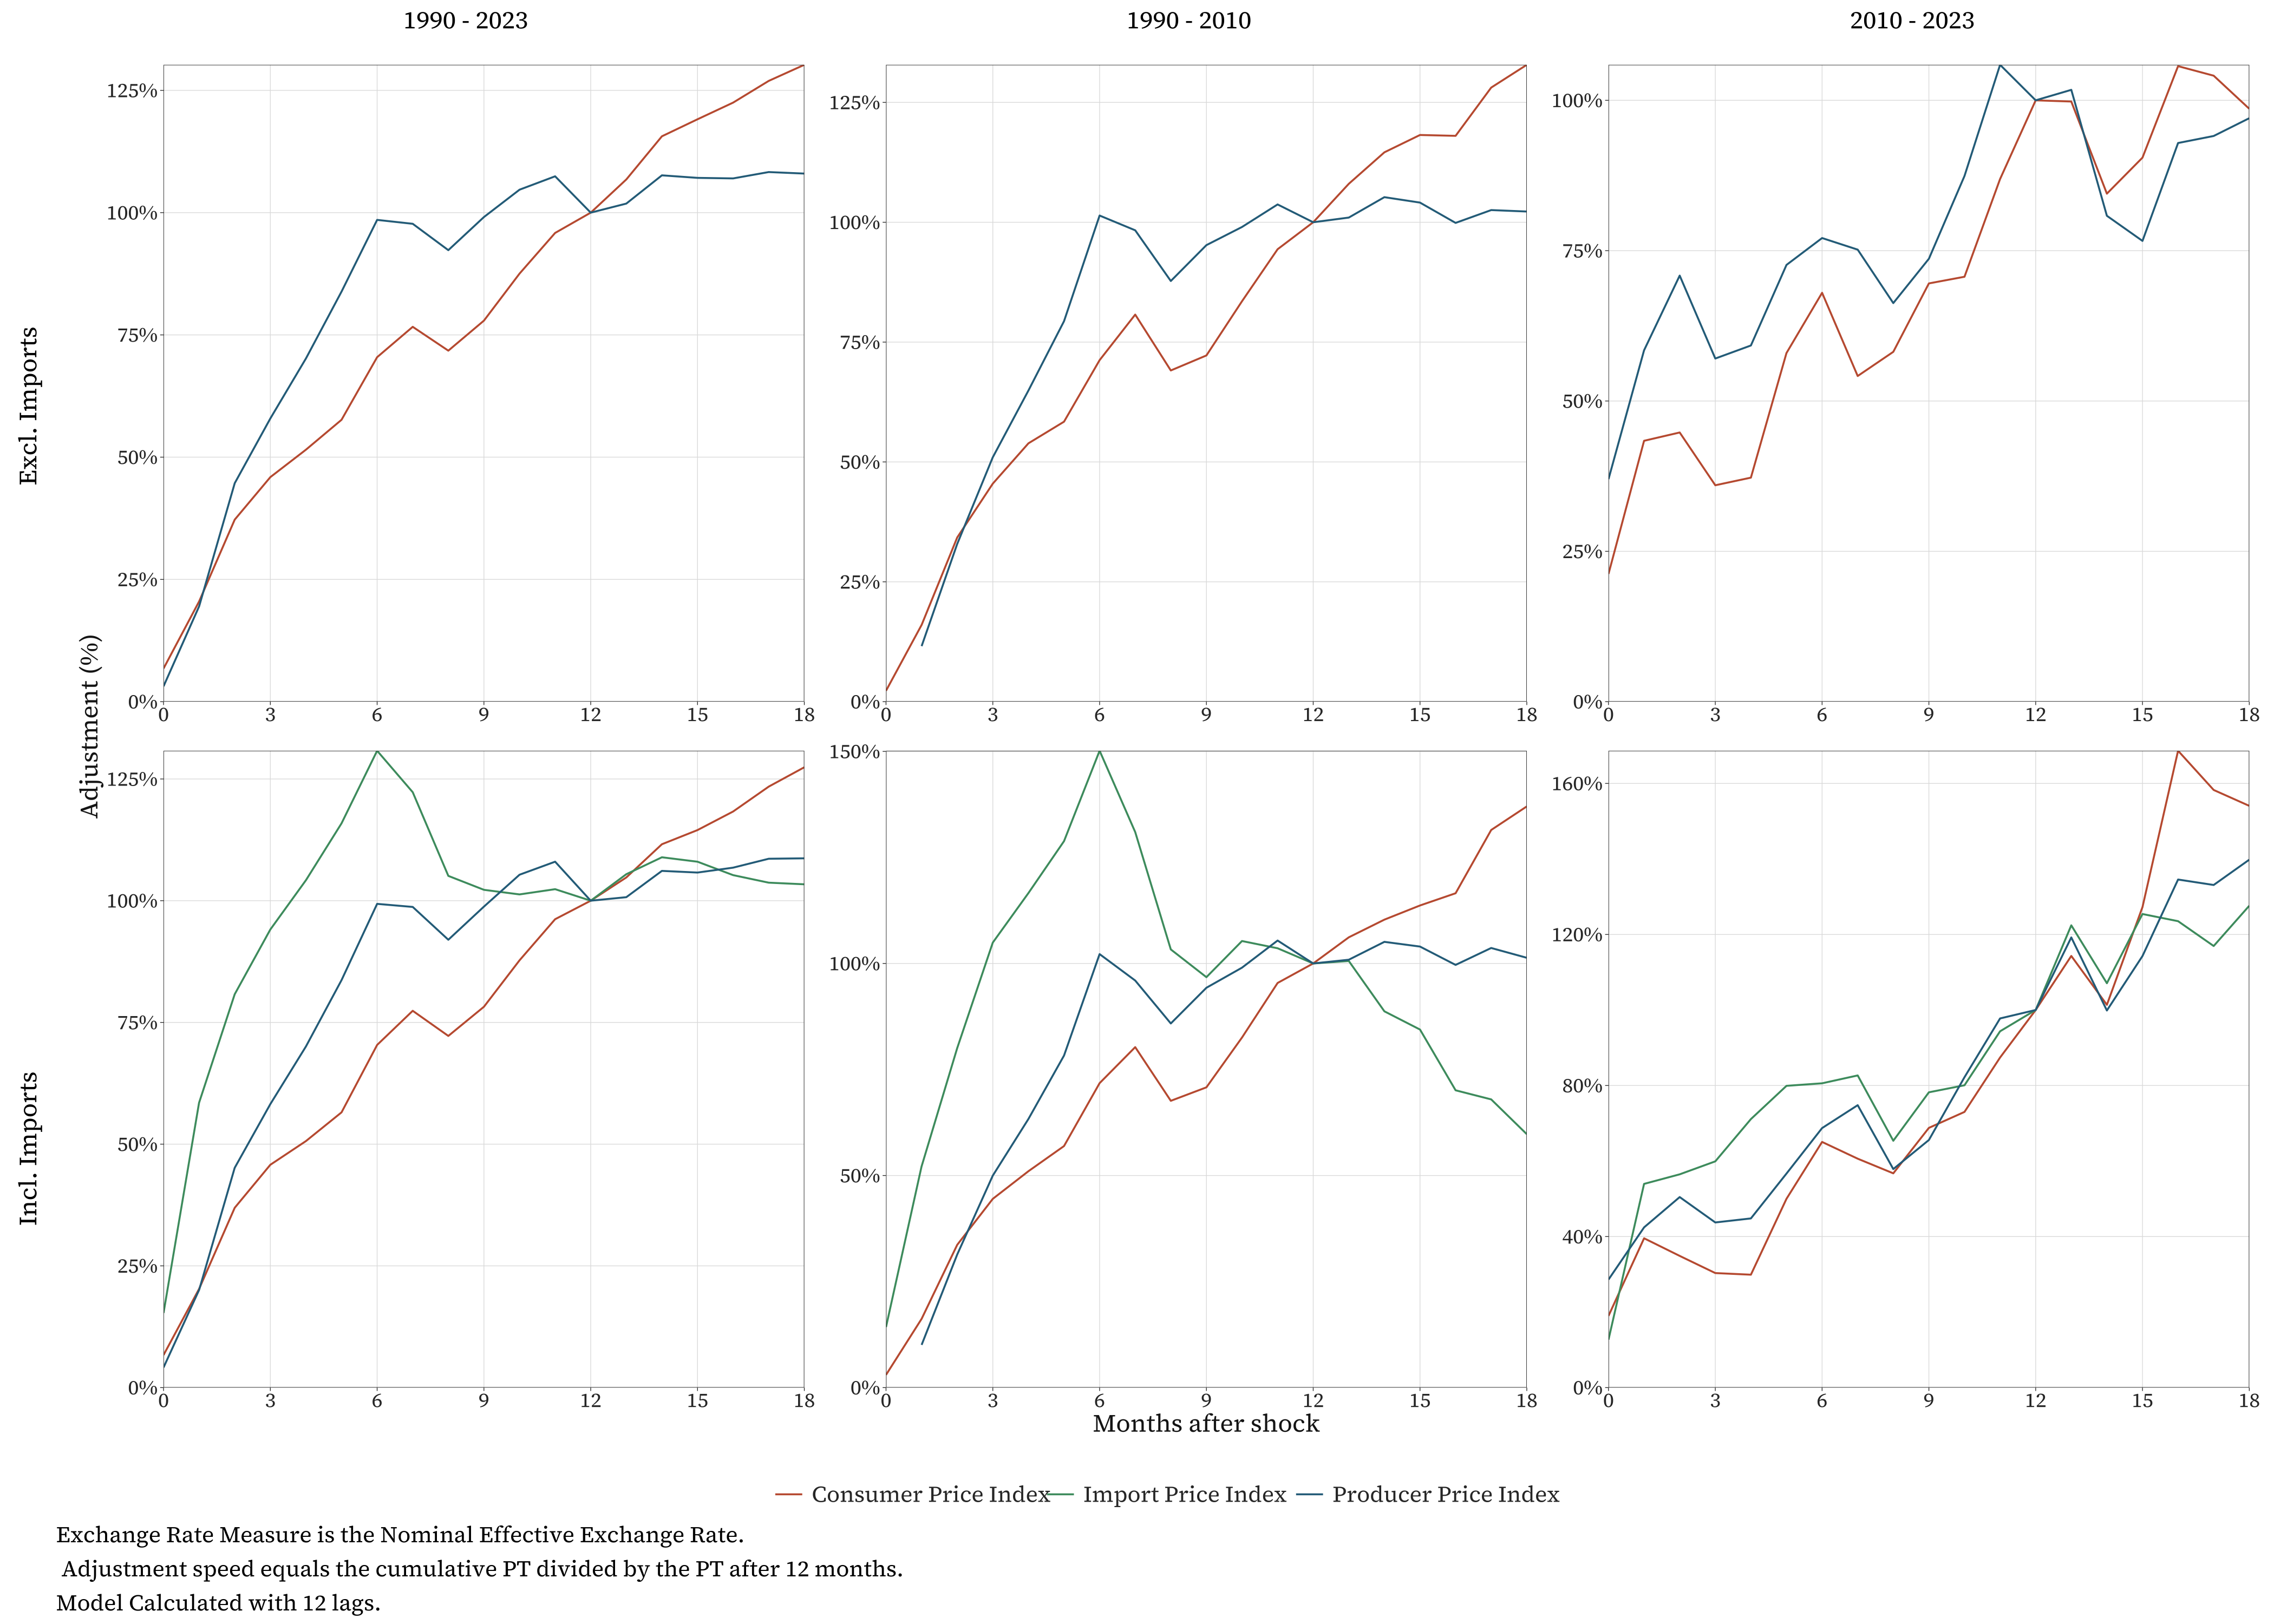
\includegraphics[width=\textwidth]{adj_p12.png}
    \caption{Adjustment Speed Plots with 12 Lags}
    \label{fig:p12_adj_plots}
\end{figure}

\input{p12_fevd.txt}

\begin{figure}[H]
    \centering
    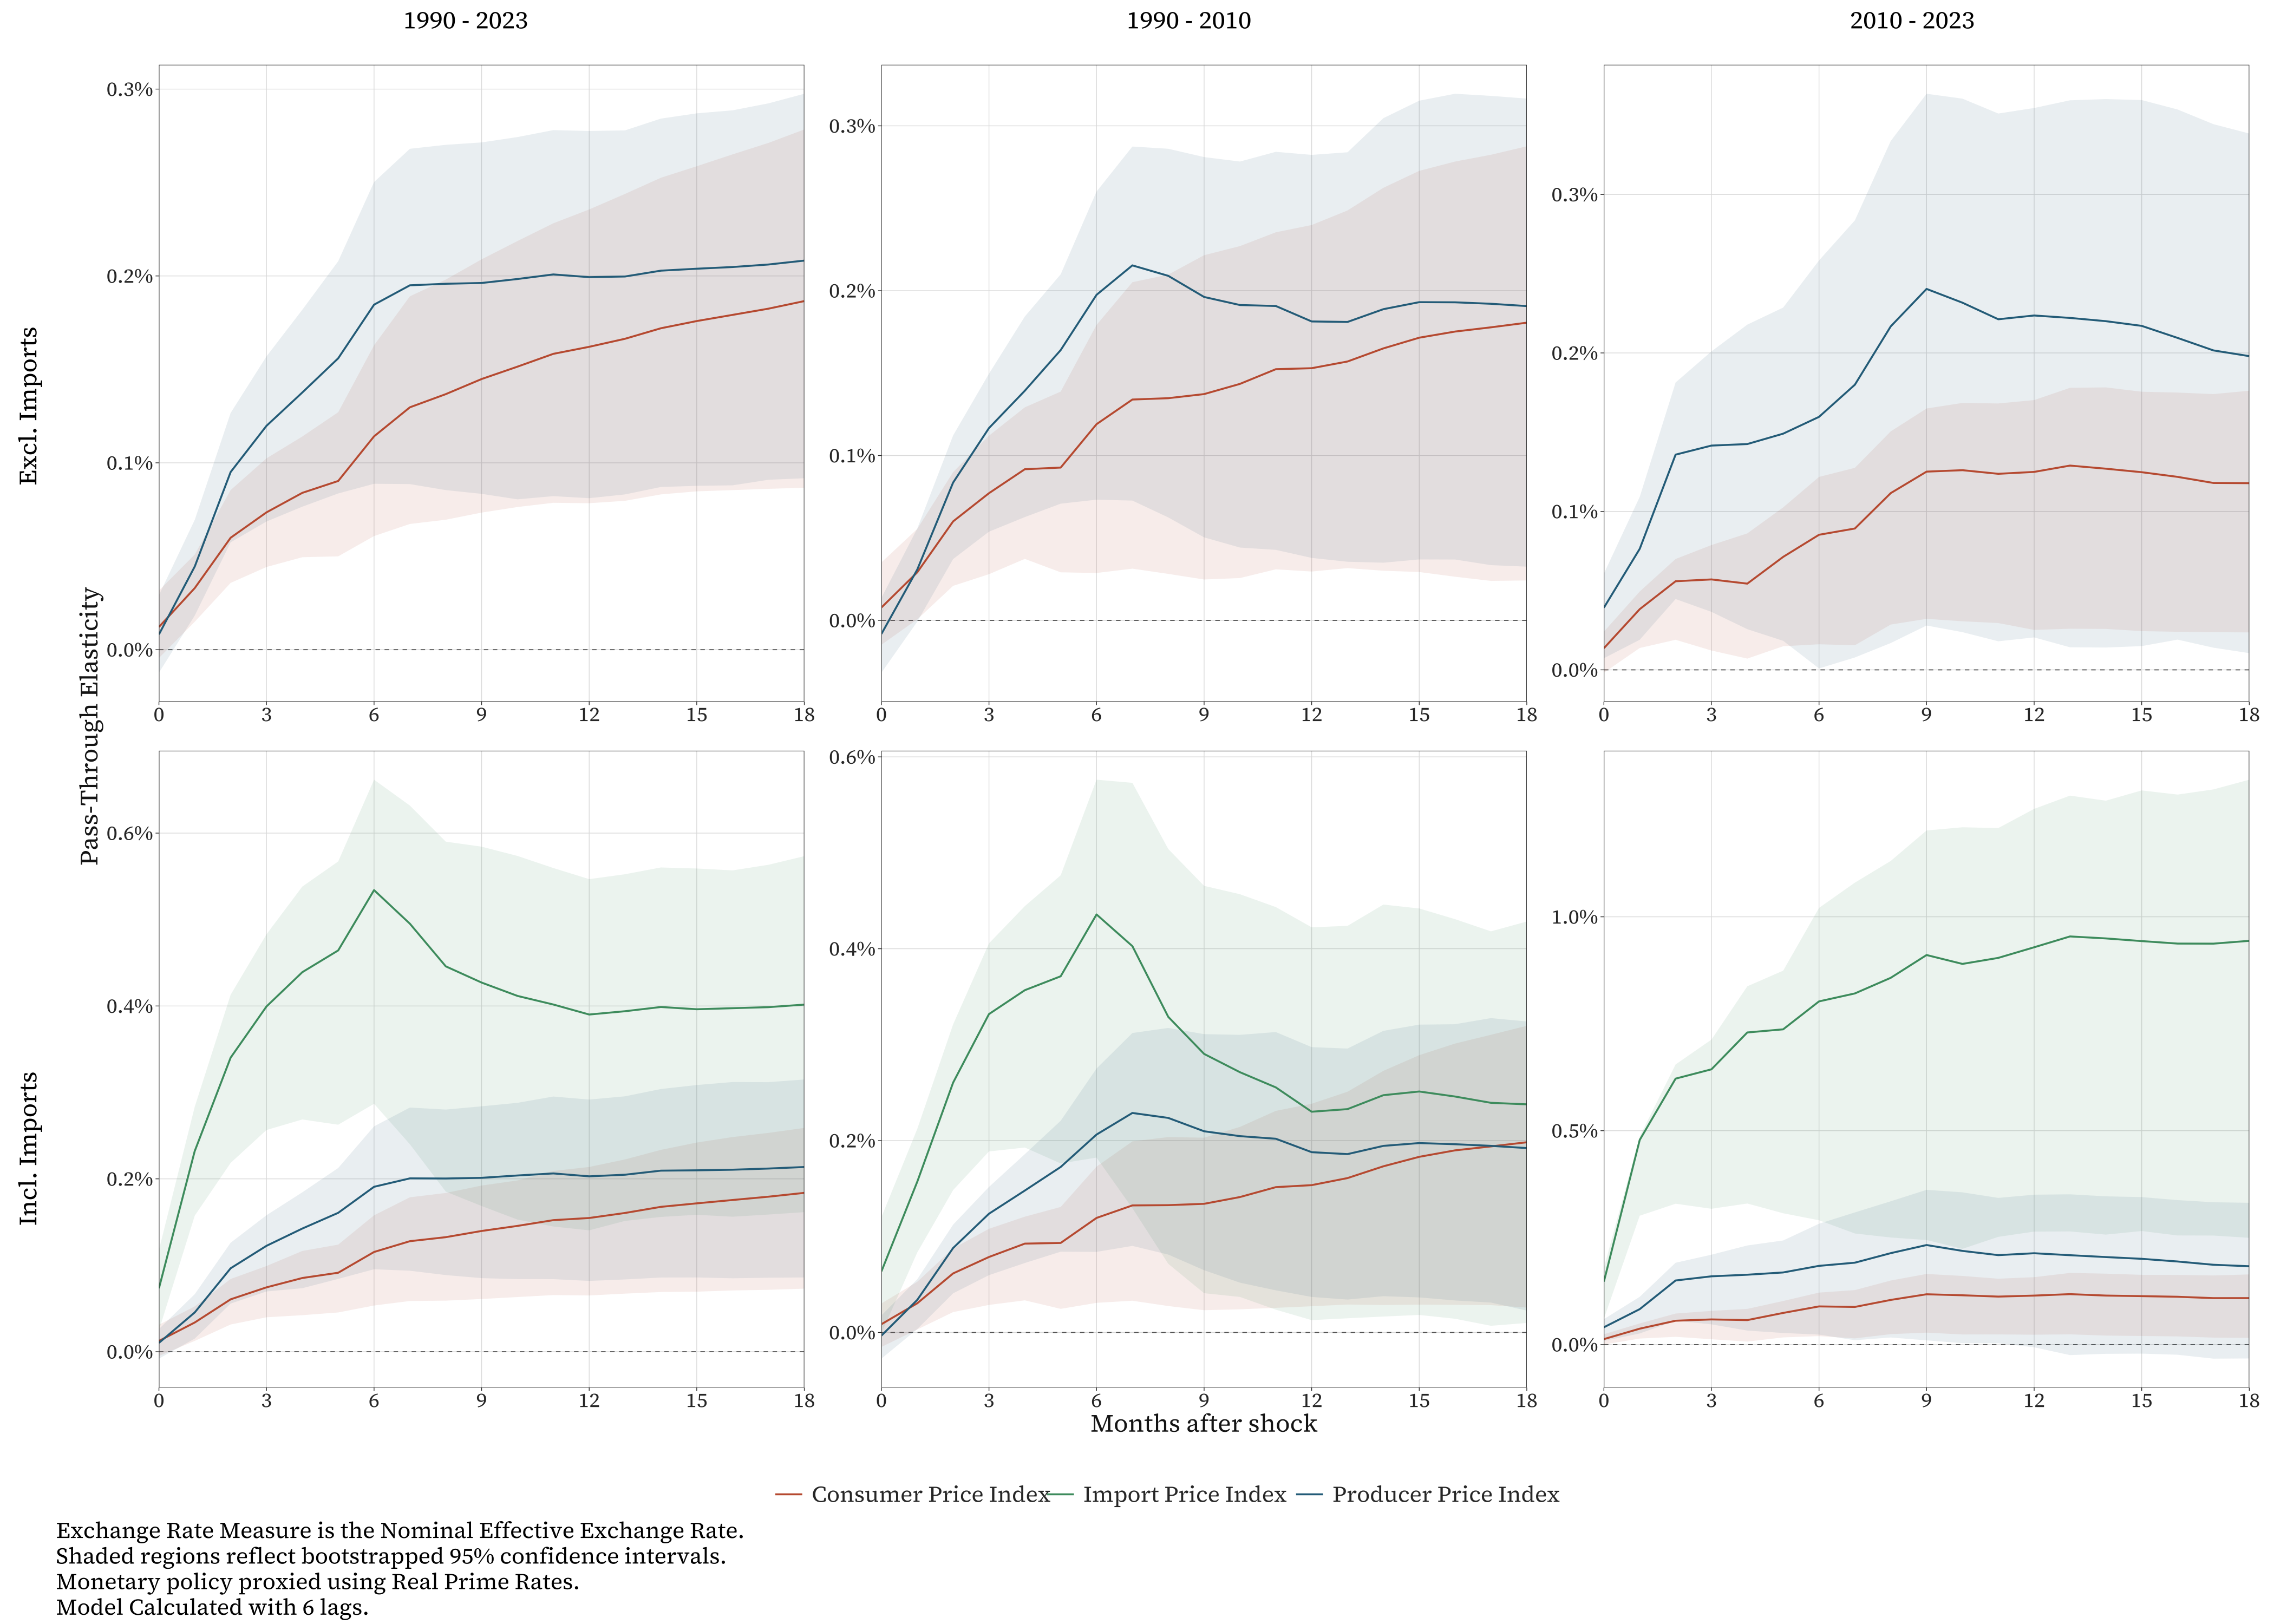
\includegraphics[width=\textwidth]{irf_monetary_policy.png}
    \caption{Impulse Response Functions with Real Prime Rates}
    \label{fig:irf_mon}
\end{figure}

\input{oil_results.txt}

\subsubsection*{A3 - Endogenous Oil}
\begin{figure}[H]
    \centering
    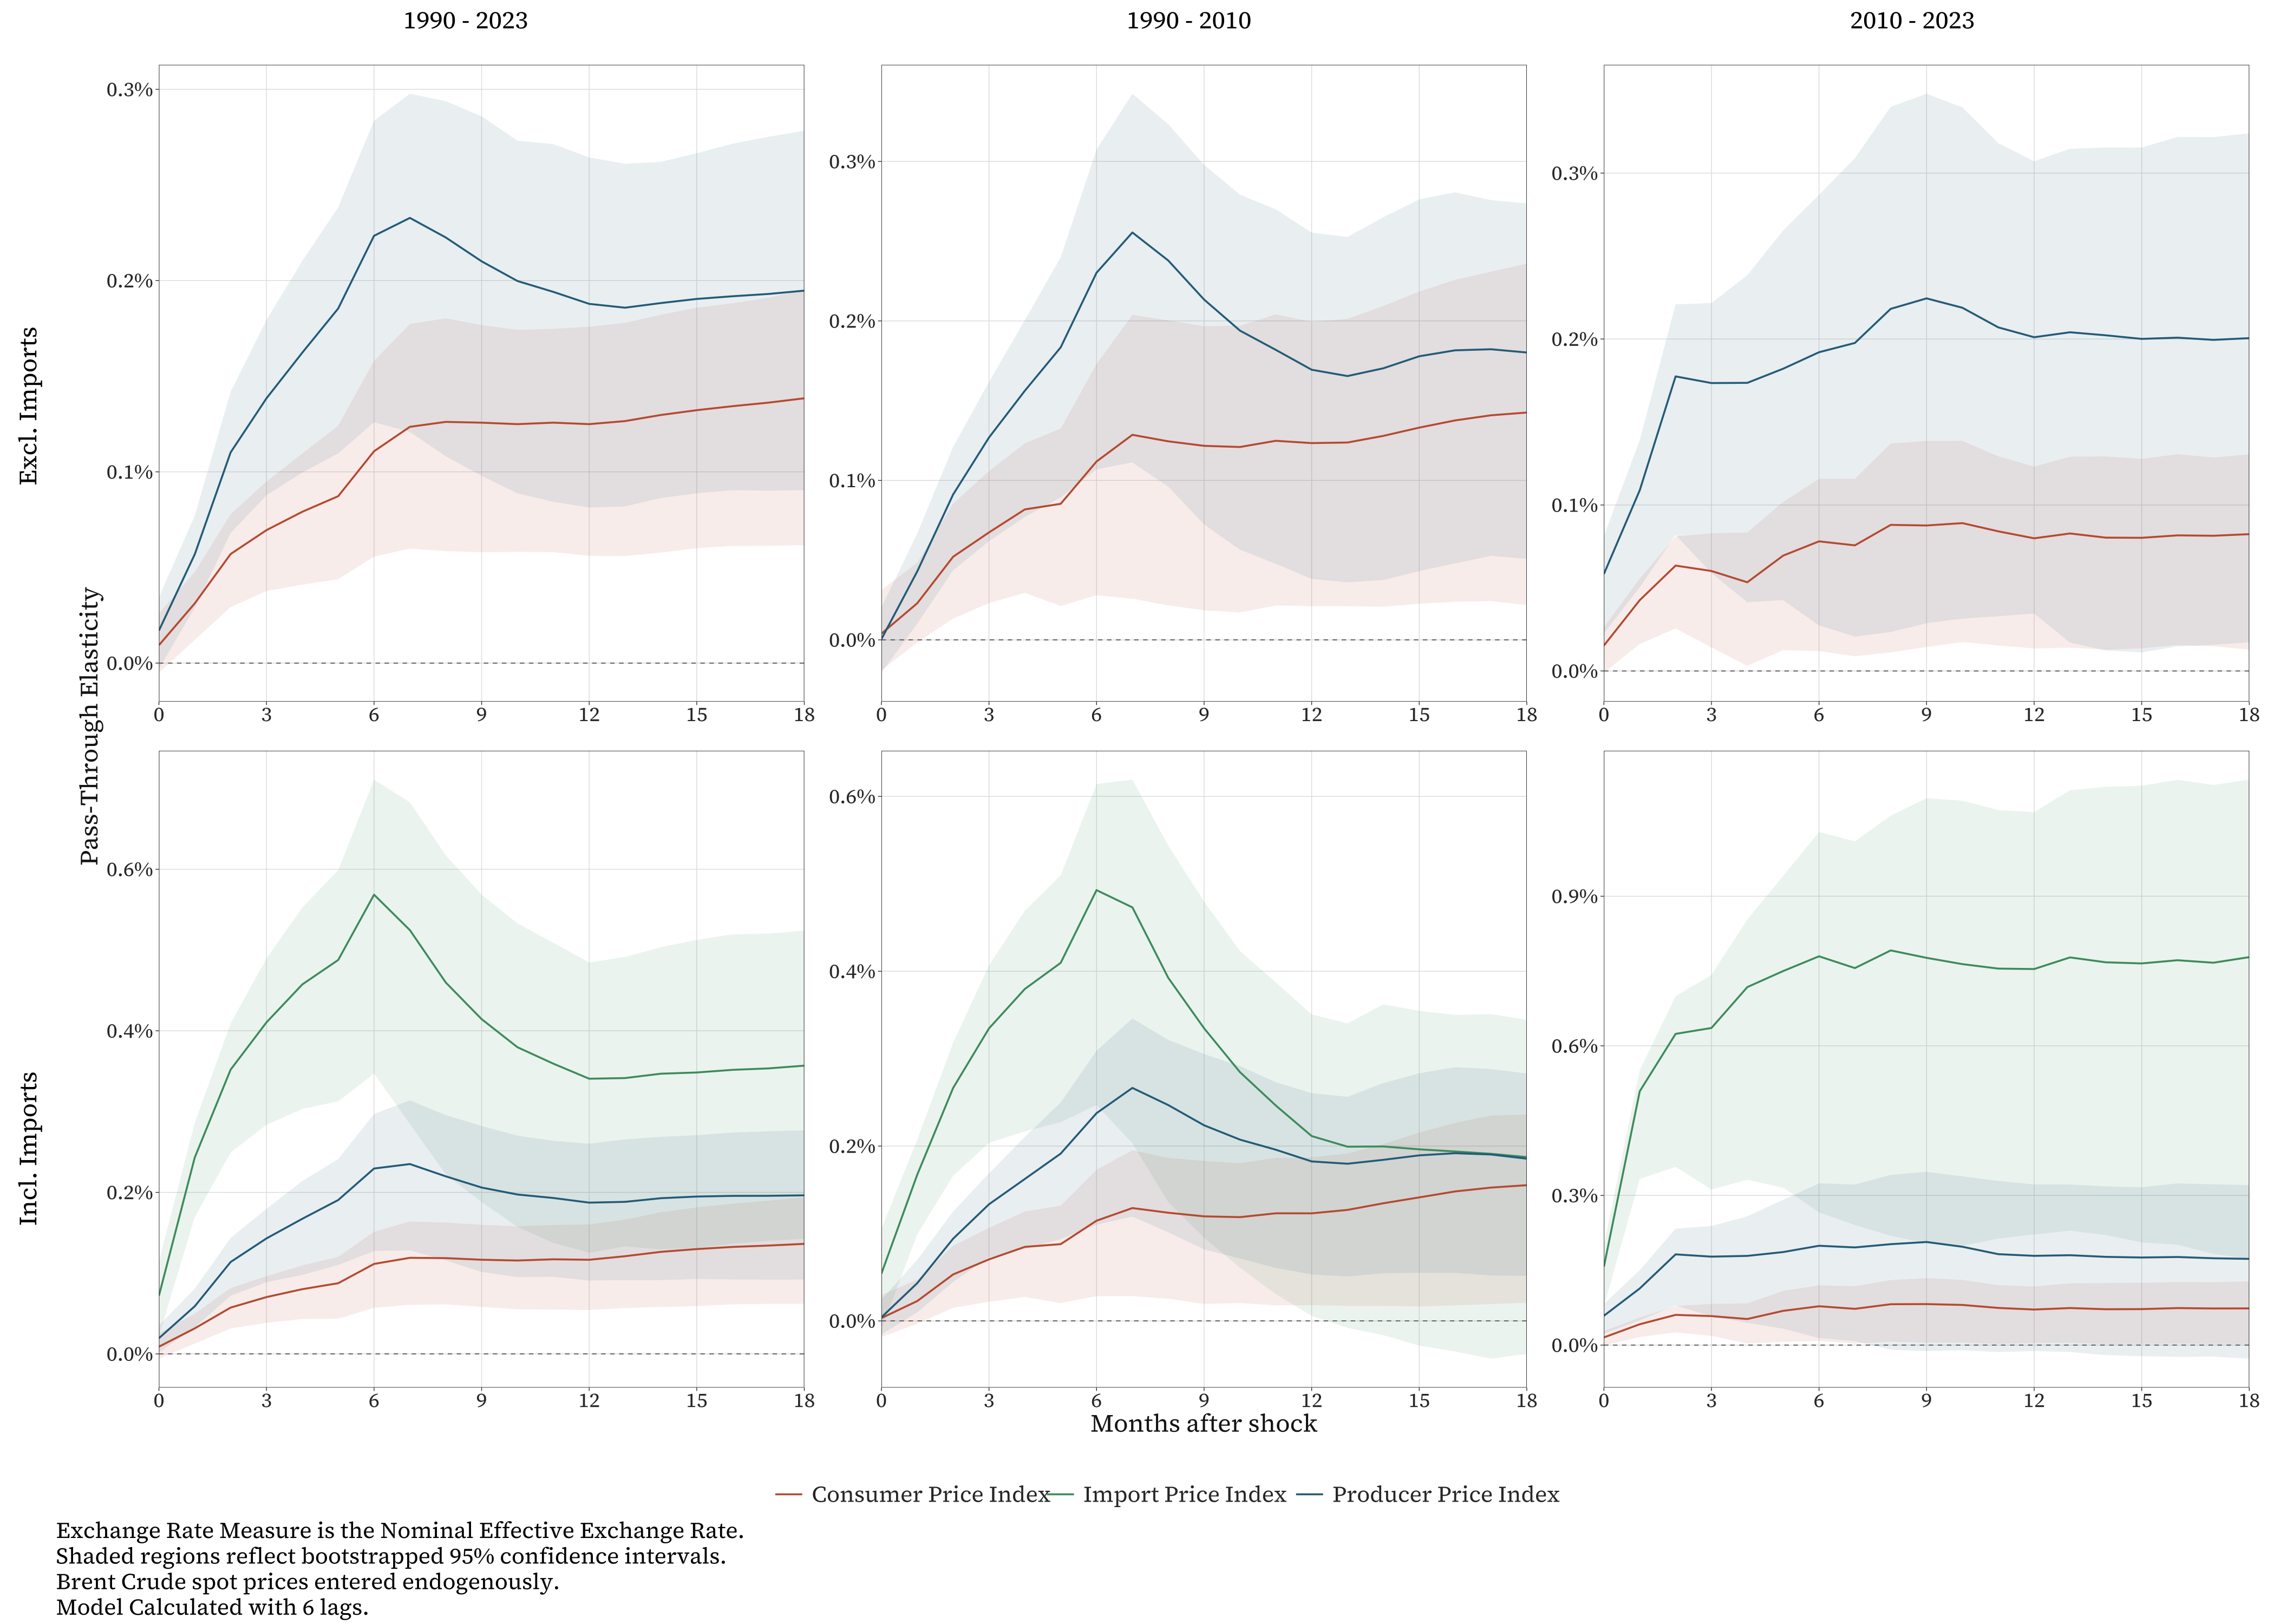
\includegraphics[width=\textwidth]{irf_oil.png}
    \caption{Impulse Response Functions with Endogenous Oil Shocks}
    \label{fig:irf_oil}
\end{figure}

\begin{figure}[H]
    \centering
    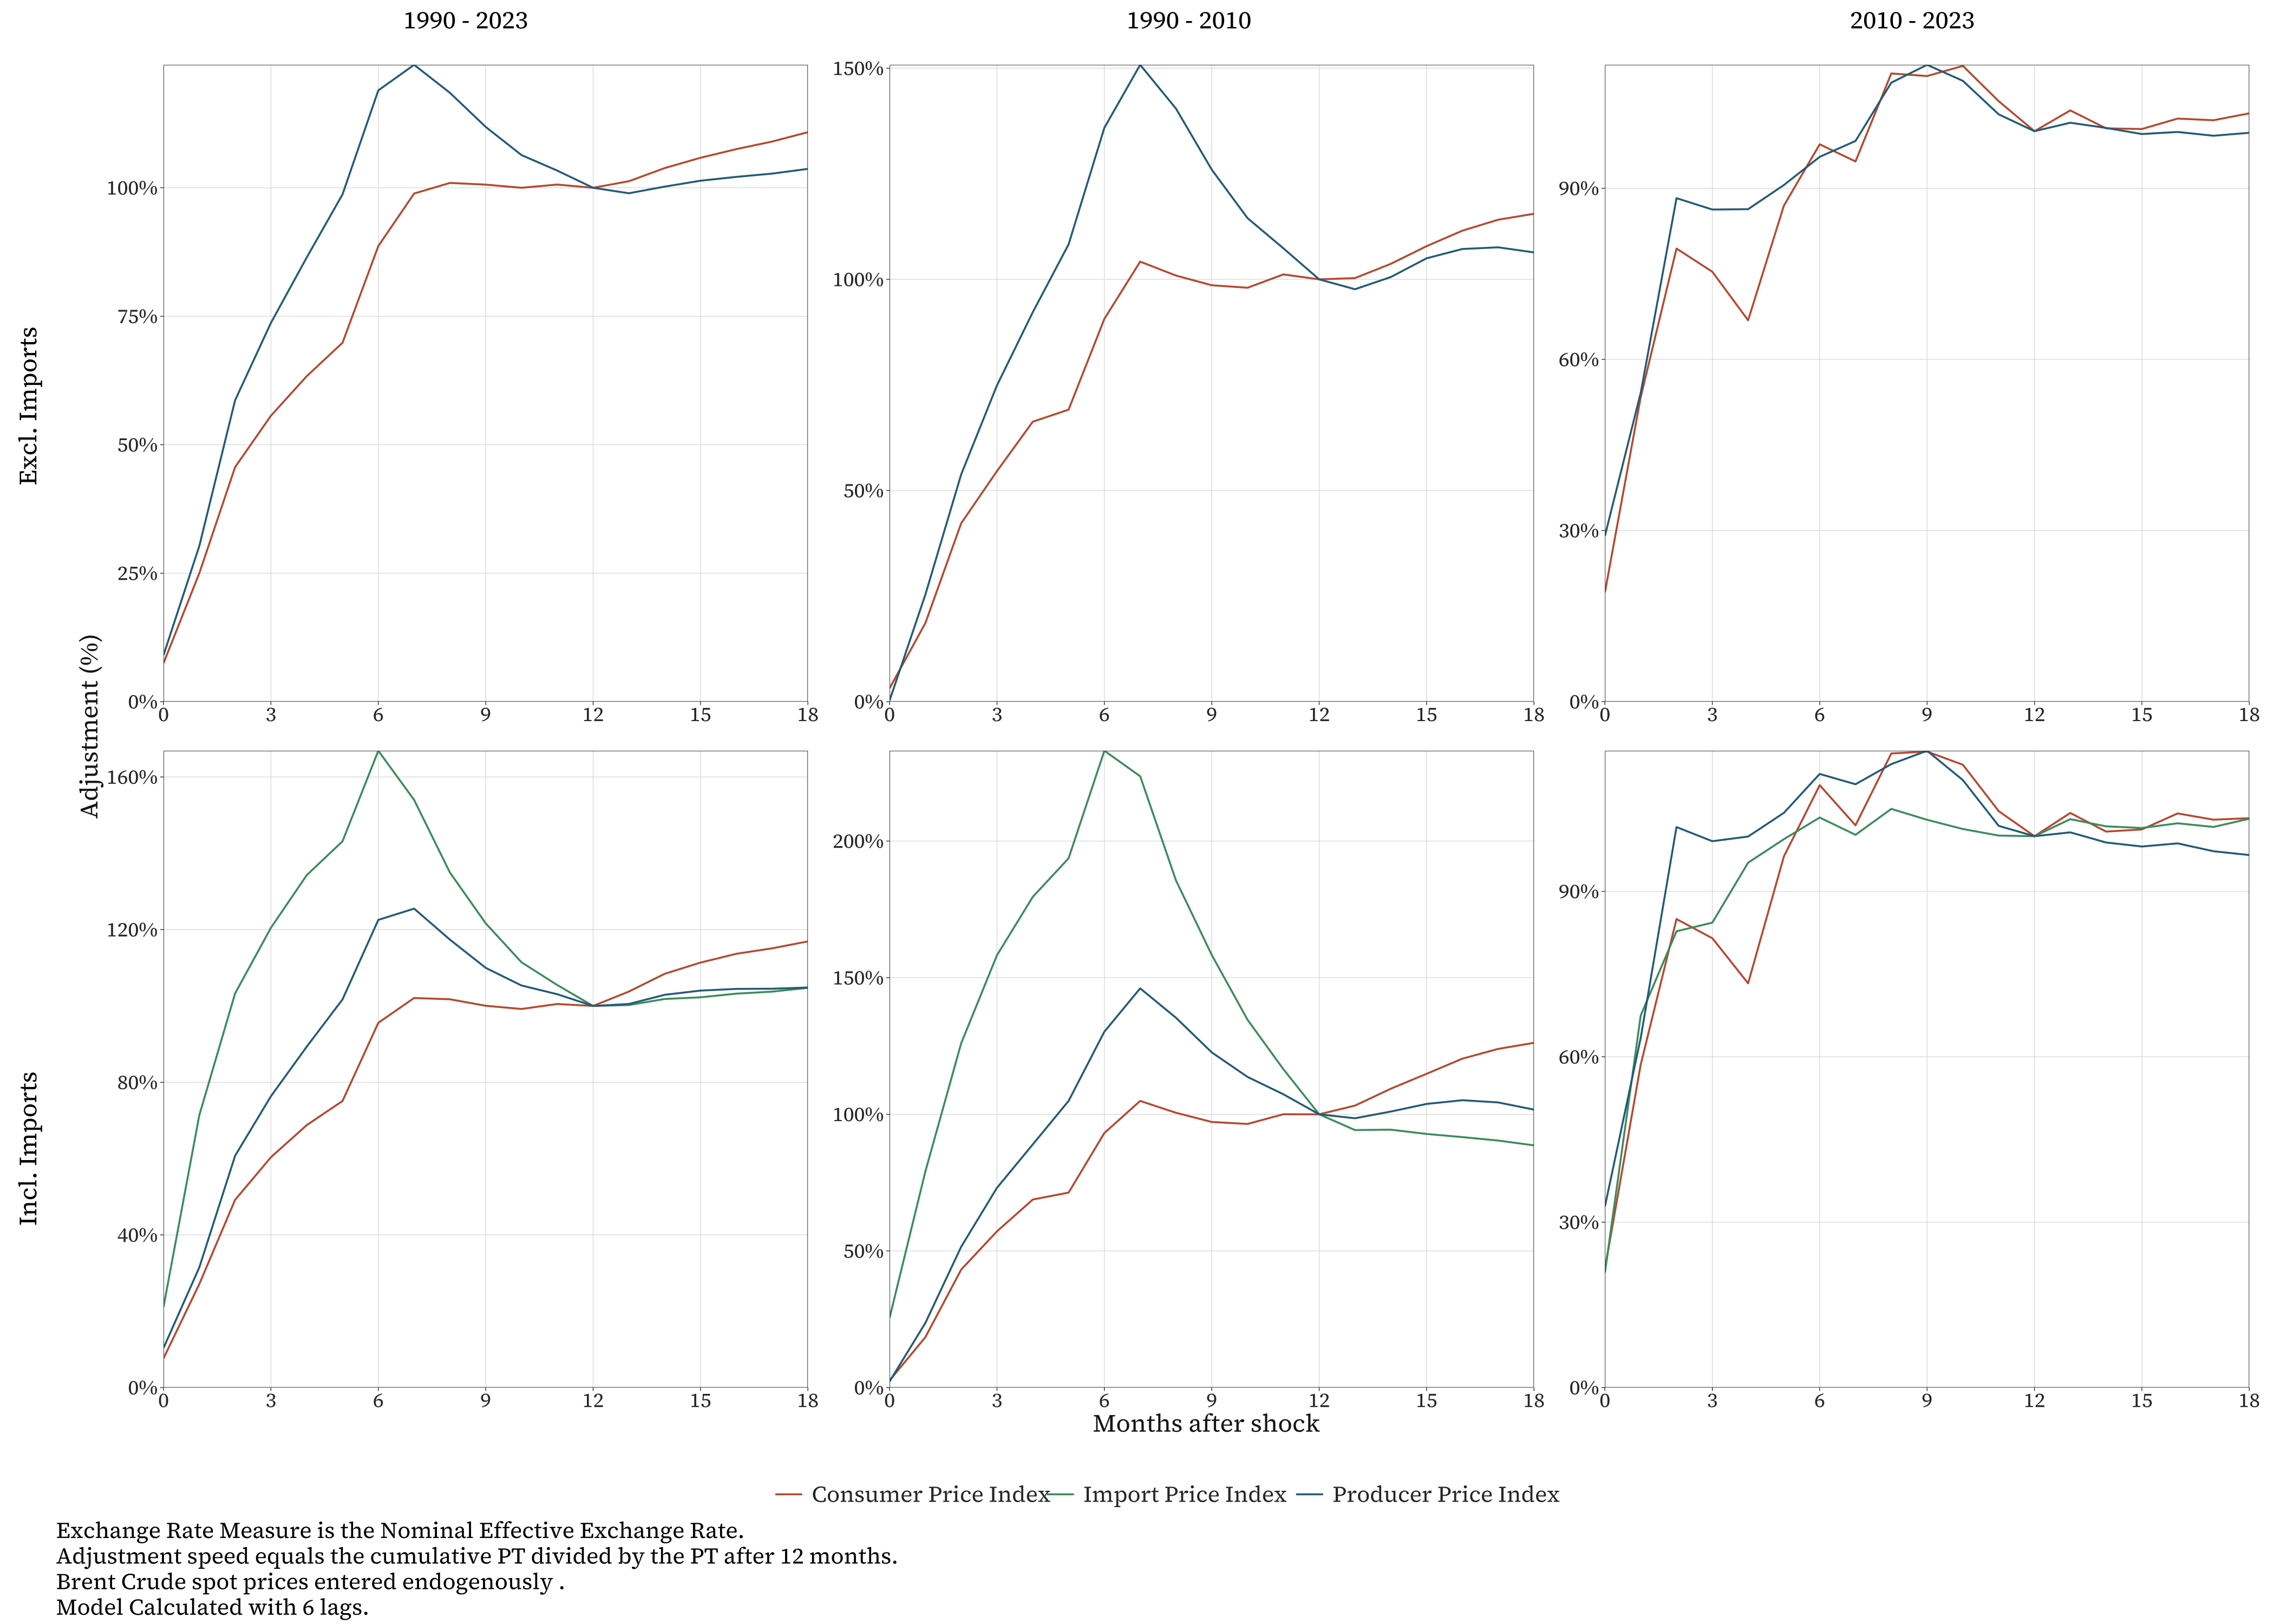
\includegraphics[width=\textwidth]{adj_oil.png}
    \caption{Adjustment Speed Plots with Endogenous Oil}
    \label{fig:oil_adj_plots}
\end{figure}

\input{oil_fevd.txt}

\subsubsection*{A4 - Monetary Policy}

\begin{figure}[H]
    \centering
    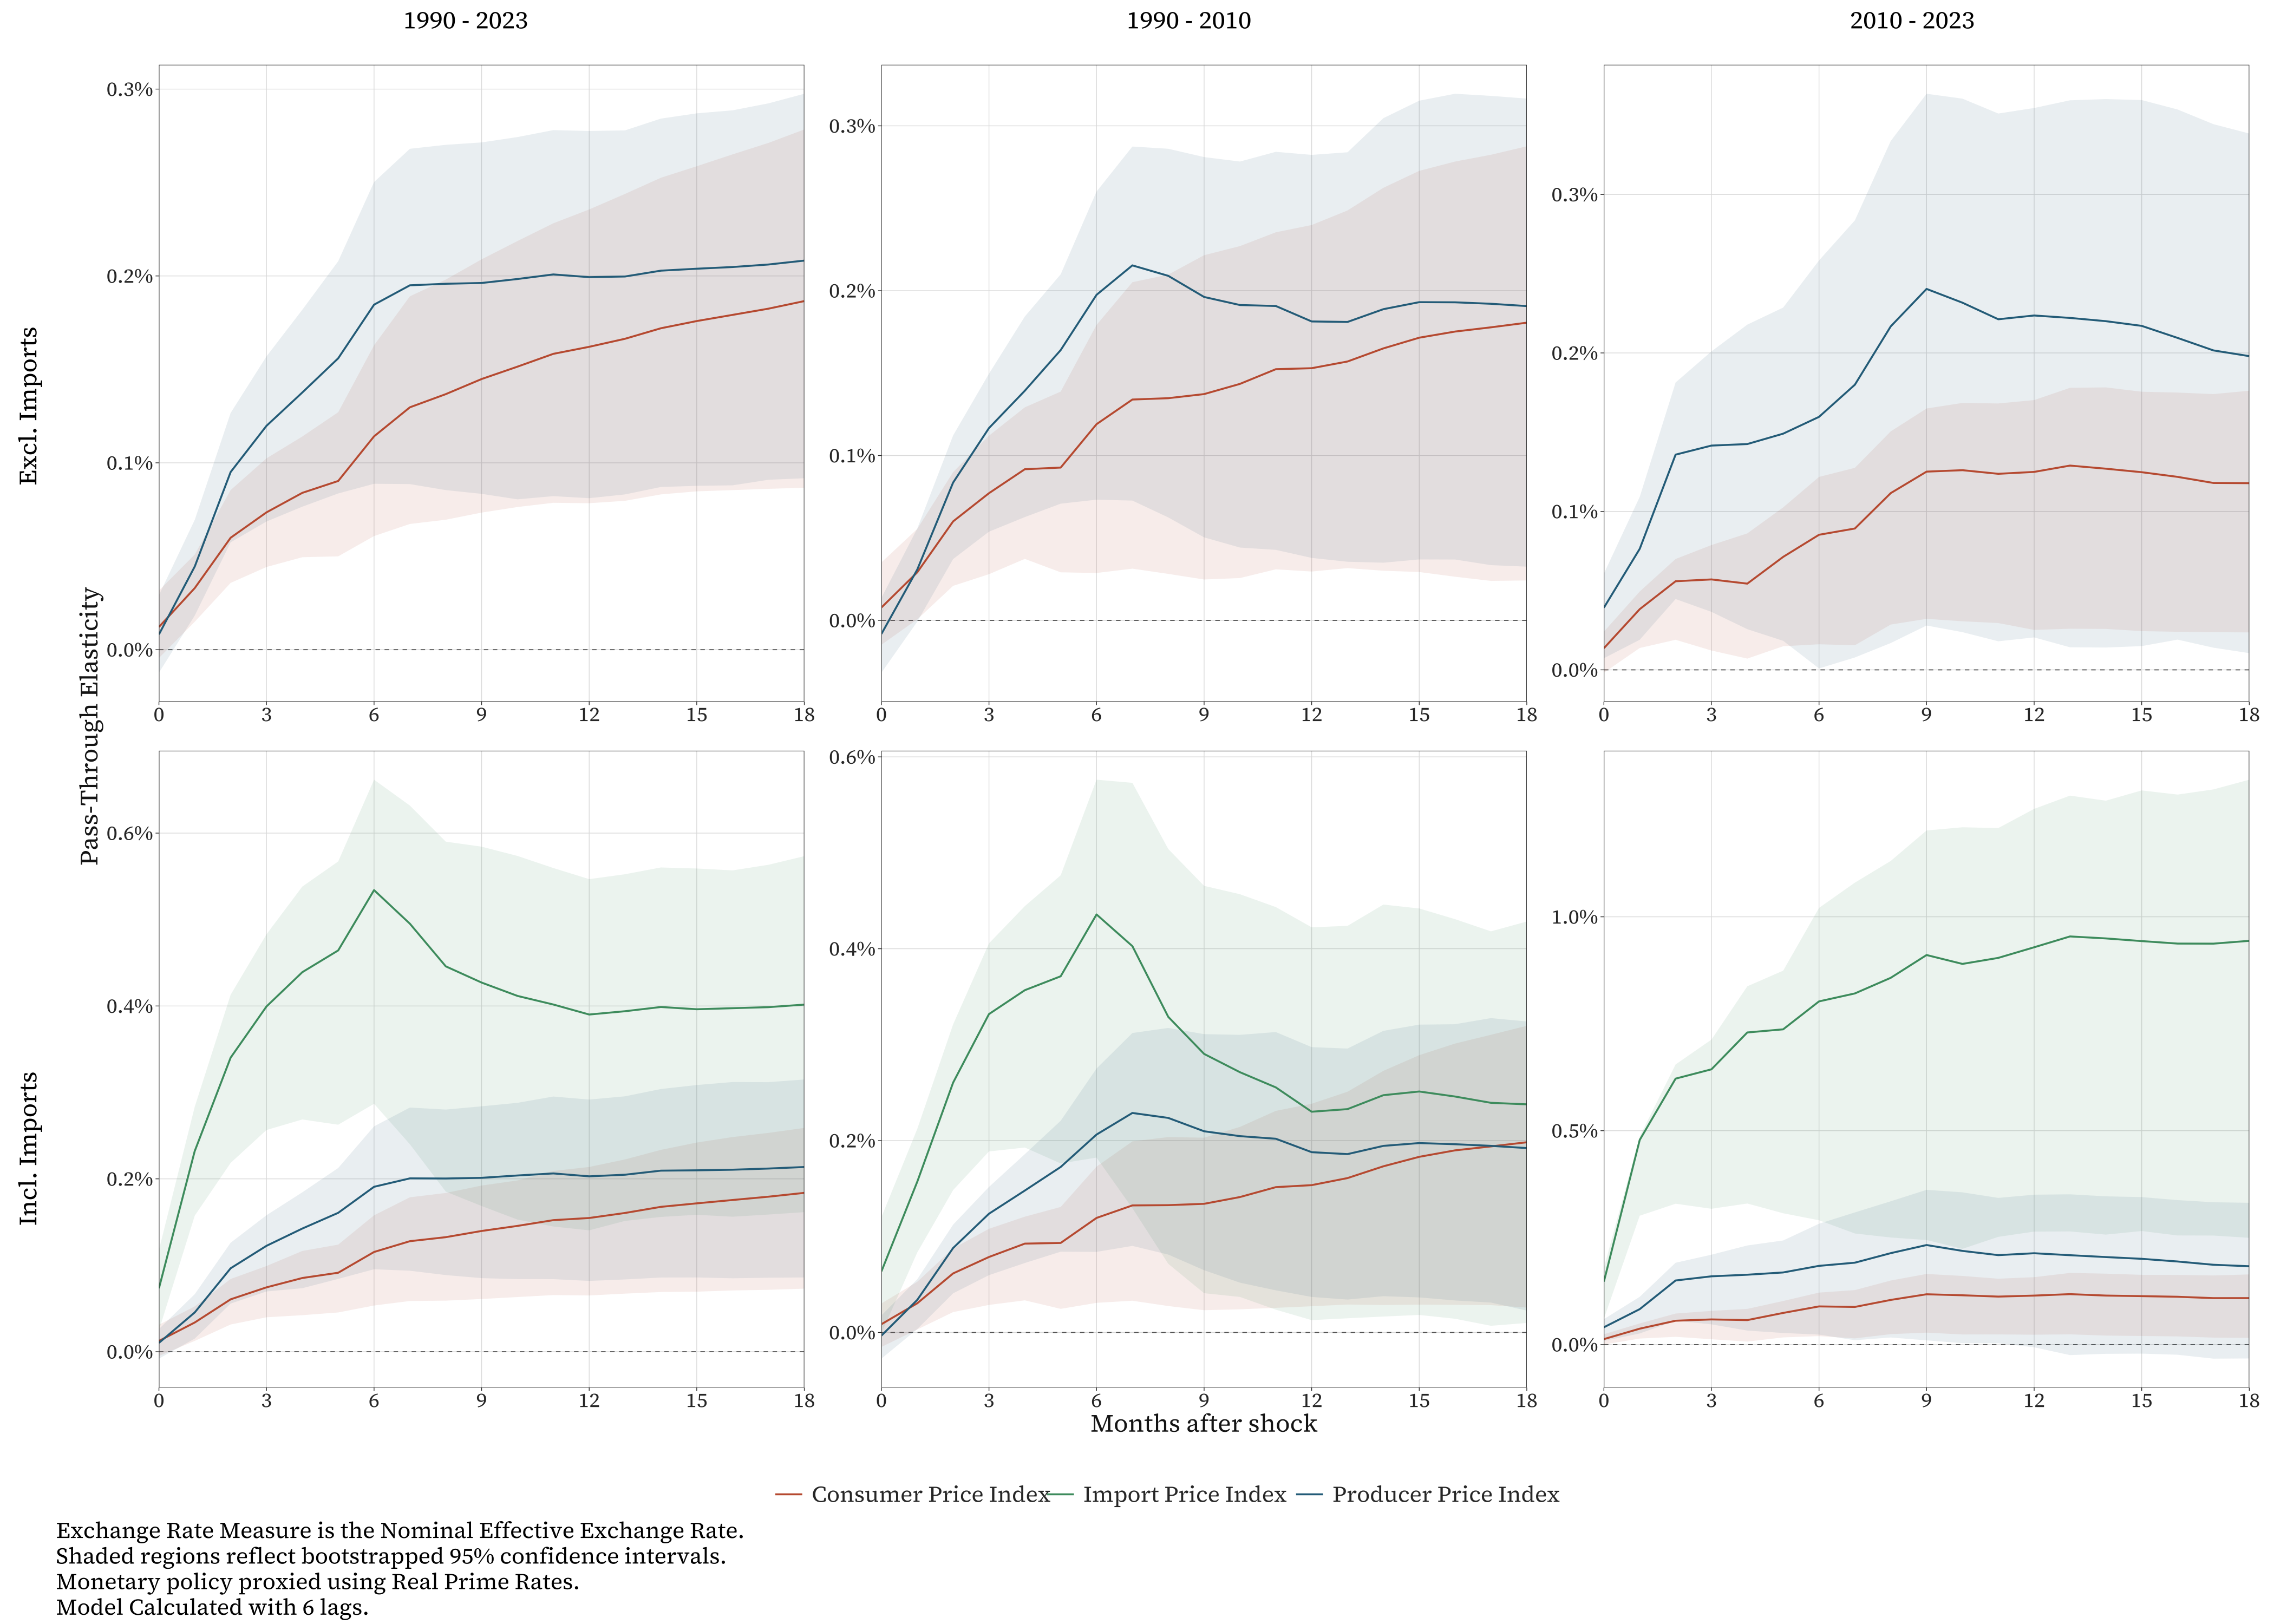
\includegraphics[width=\textwidth]{irf_monetary_policy.png}
    \caption{Impulse Response Functions with Real Prime Rates}
    \label{fig:irf_p12}
\end{figure}

\input{monetary_results.txt}


\begin{figure}[H]
    \centering
    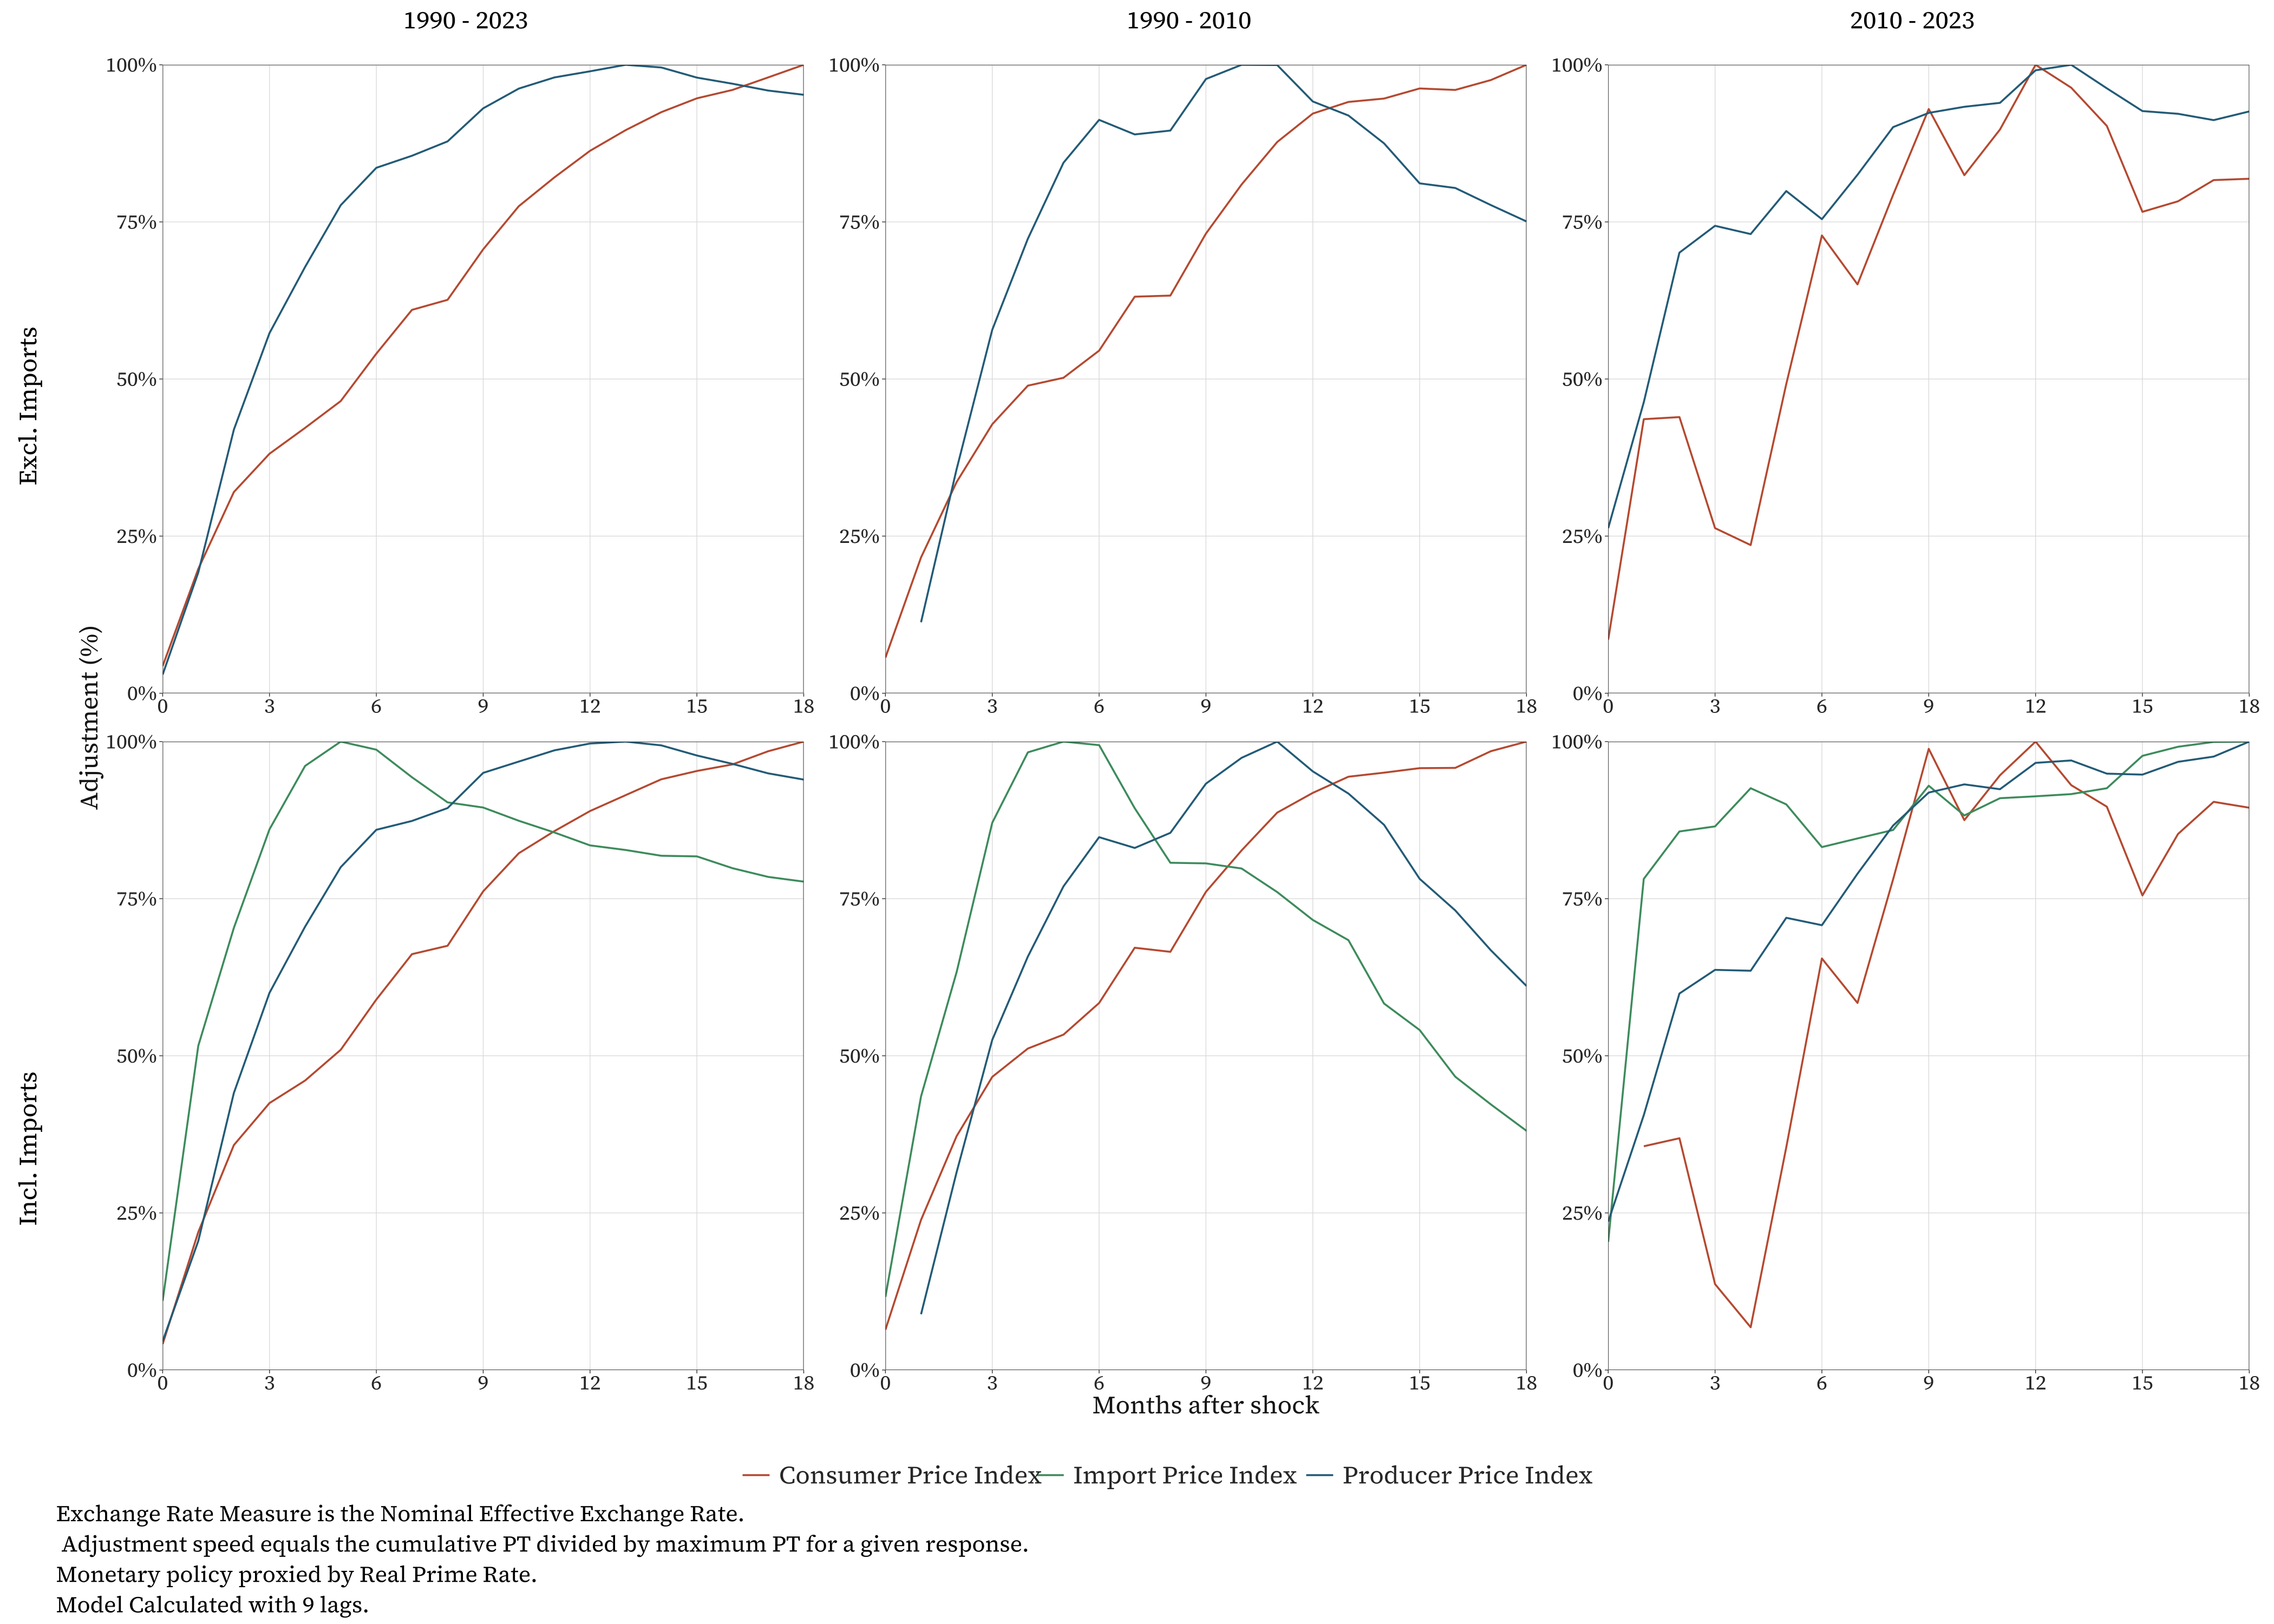
\includegraphics[width=\textwidth]{adj_monetary_policy.png}
    \caption{Adjustment Speed Plots with Real Prime Rates}
    \label{fig:monetary_adj_plots}
\end{figure}

\input{monetary_fevd.txt}

\subsubsection*{A5 - Linear Projections}

\begin{figure}[H]
    \centering
    
\includegraphics[width=\textwidth]{irf_lp.png}
    \caption{Impulse Response Functions using Linear Projections}
    \label{fig:irf_lp}
\end{figure}

\input{lp_results.txt}


\begin{figure}[H]
    \centering
    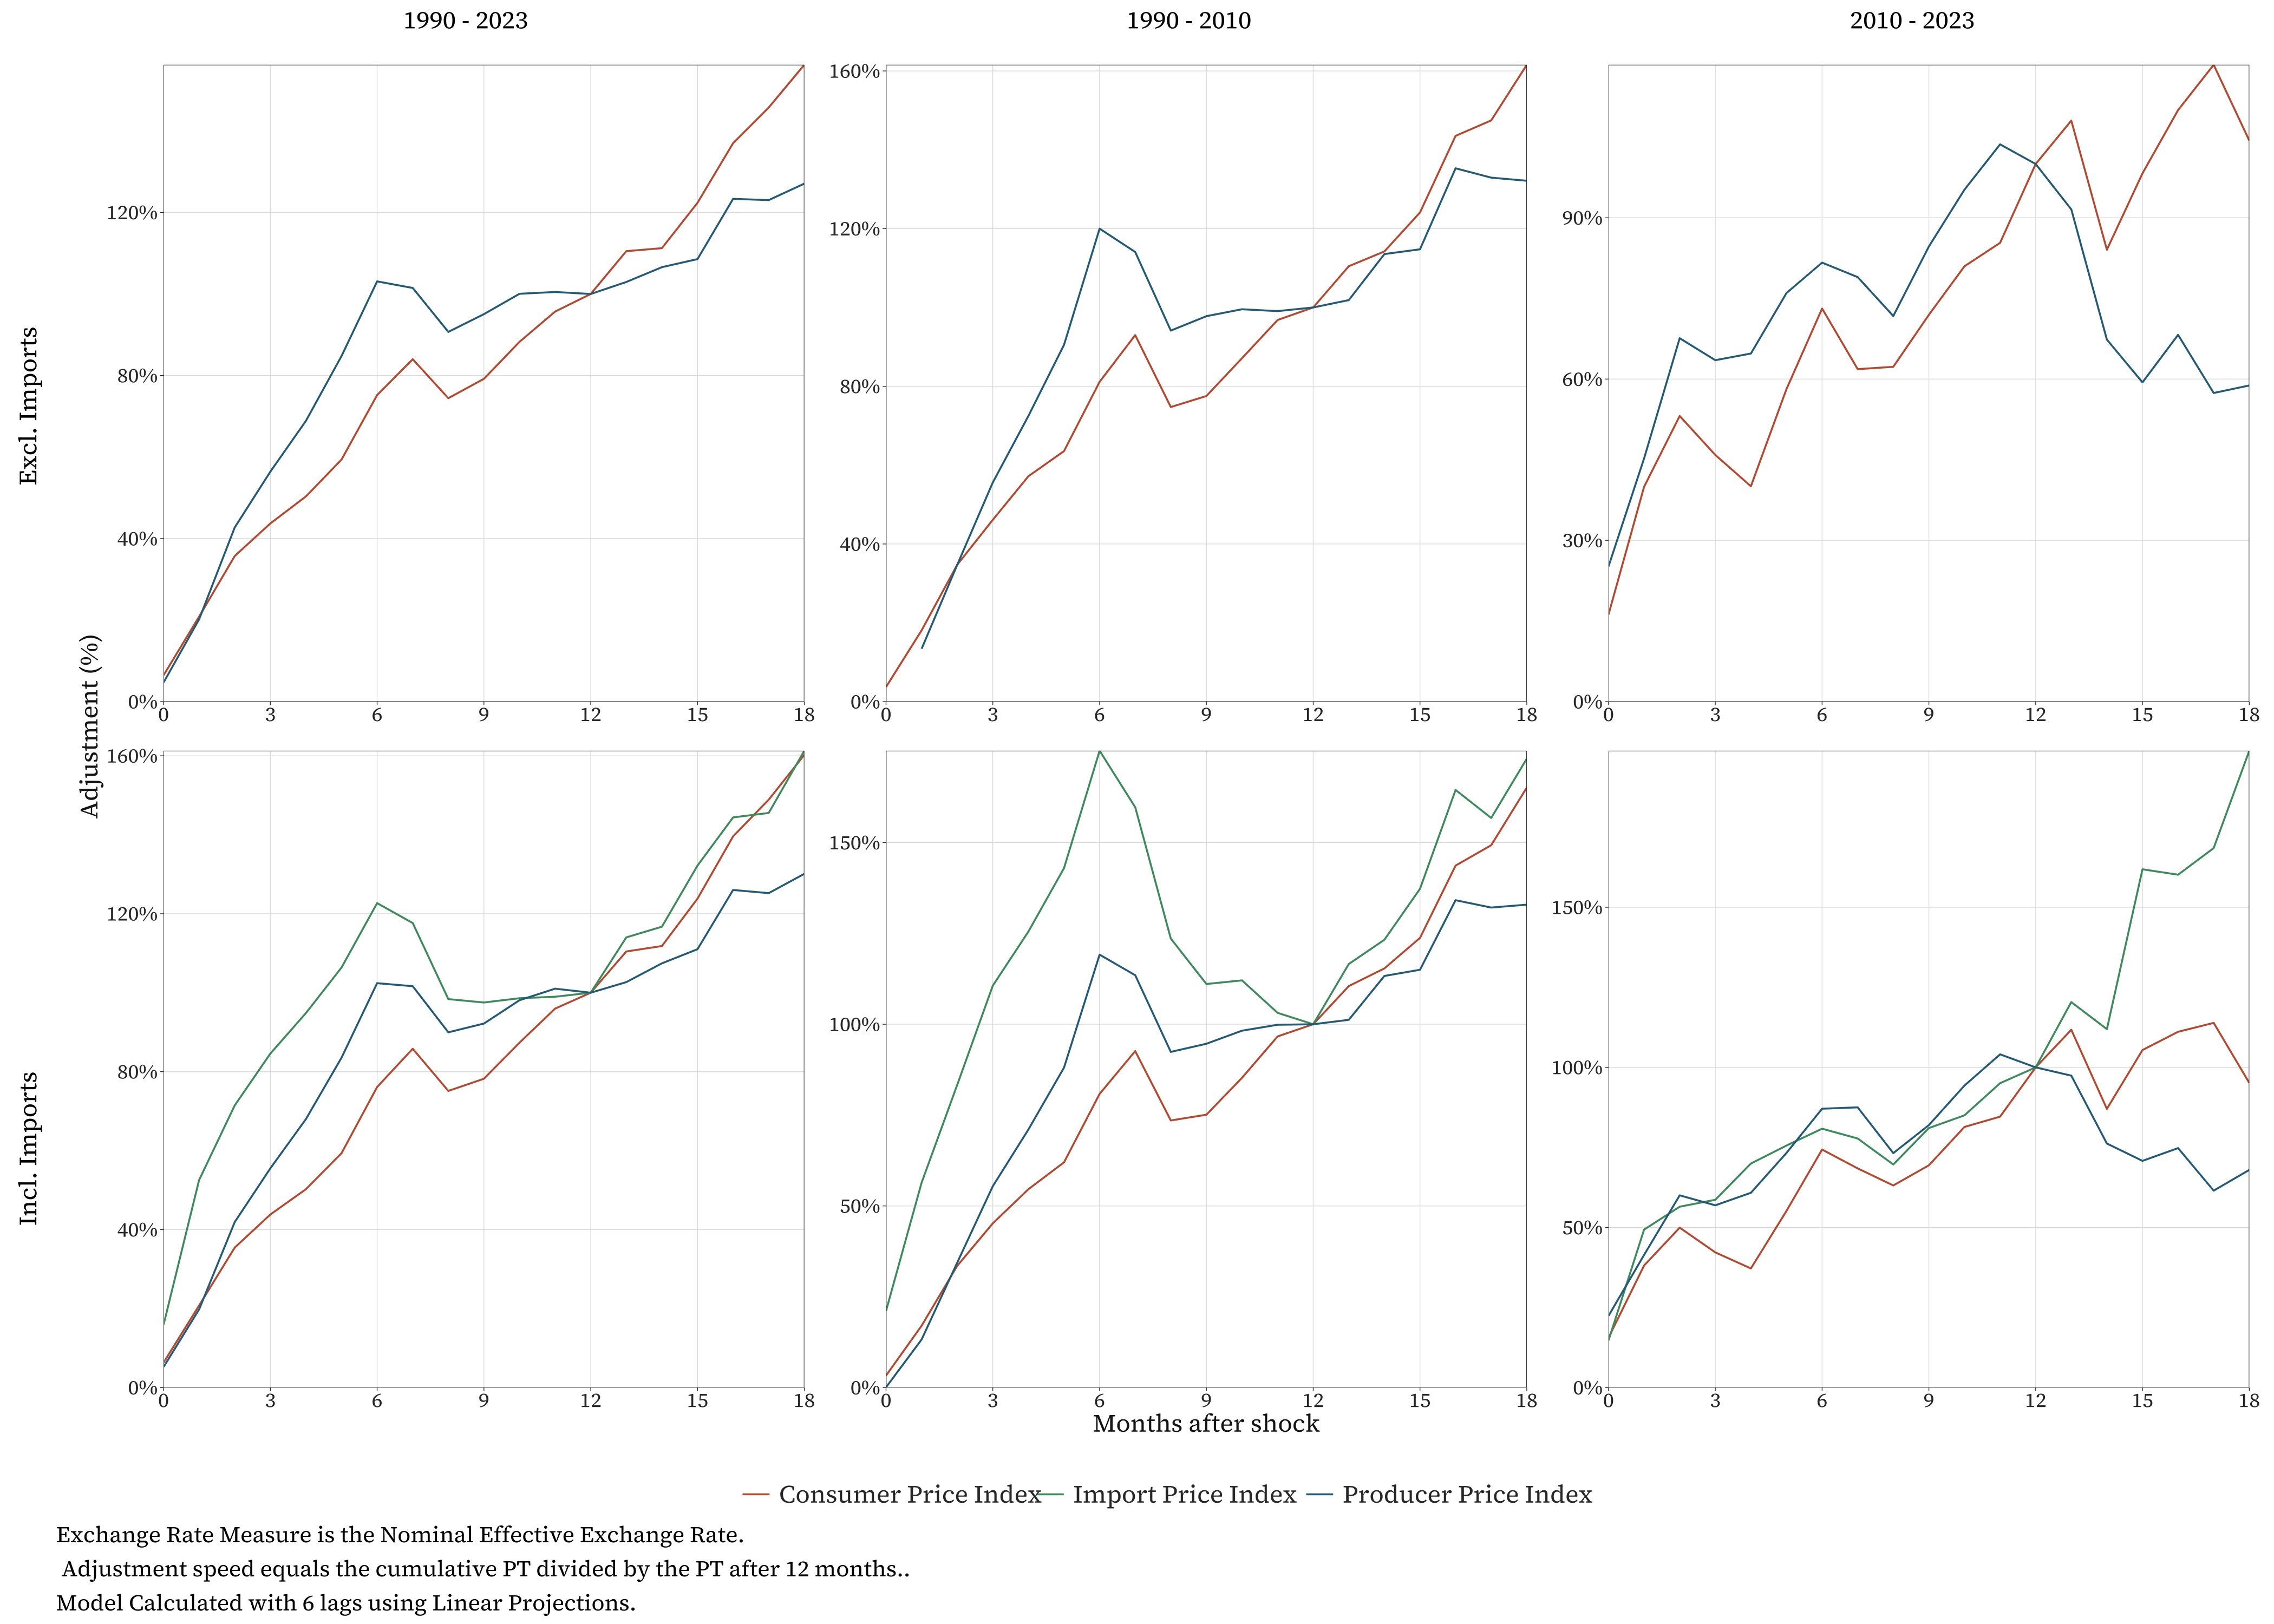
\includegraphics[width=\textwidth]{adj_lp.png}
    \caption{Adjustment Speed Plots using Linear Projections}
    \label{fig:lp_adj_plots}
\end{figure}


\subsection*{Appendix B - Diagnostics}

\subsection*{B2 - Descriptives}


\input{desc_tbl.txt}

\subsection*{B2 - Chow-Lin Disaggregation}

\input{chow_lin.txt}

\subsubsection*{B3 - Stationarity}

\begin{figure}[H]
    \centering
    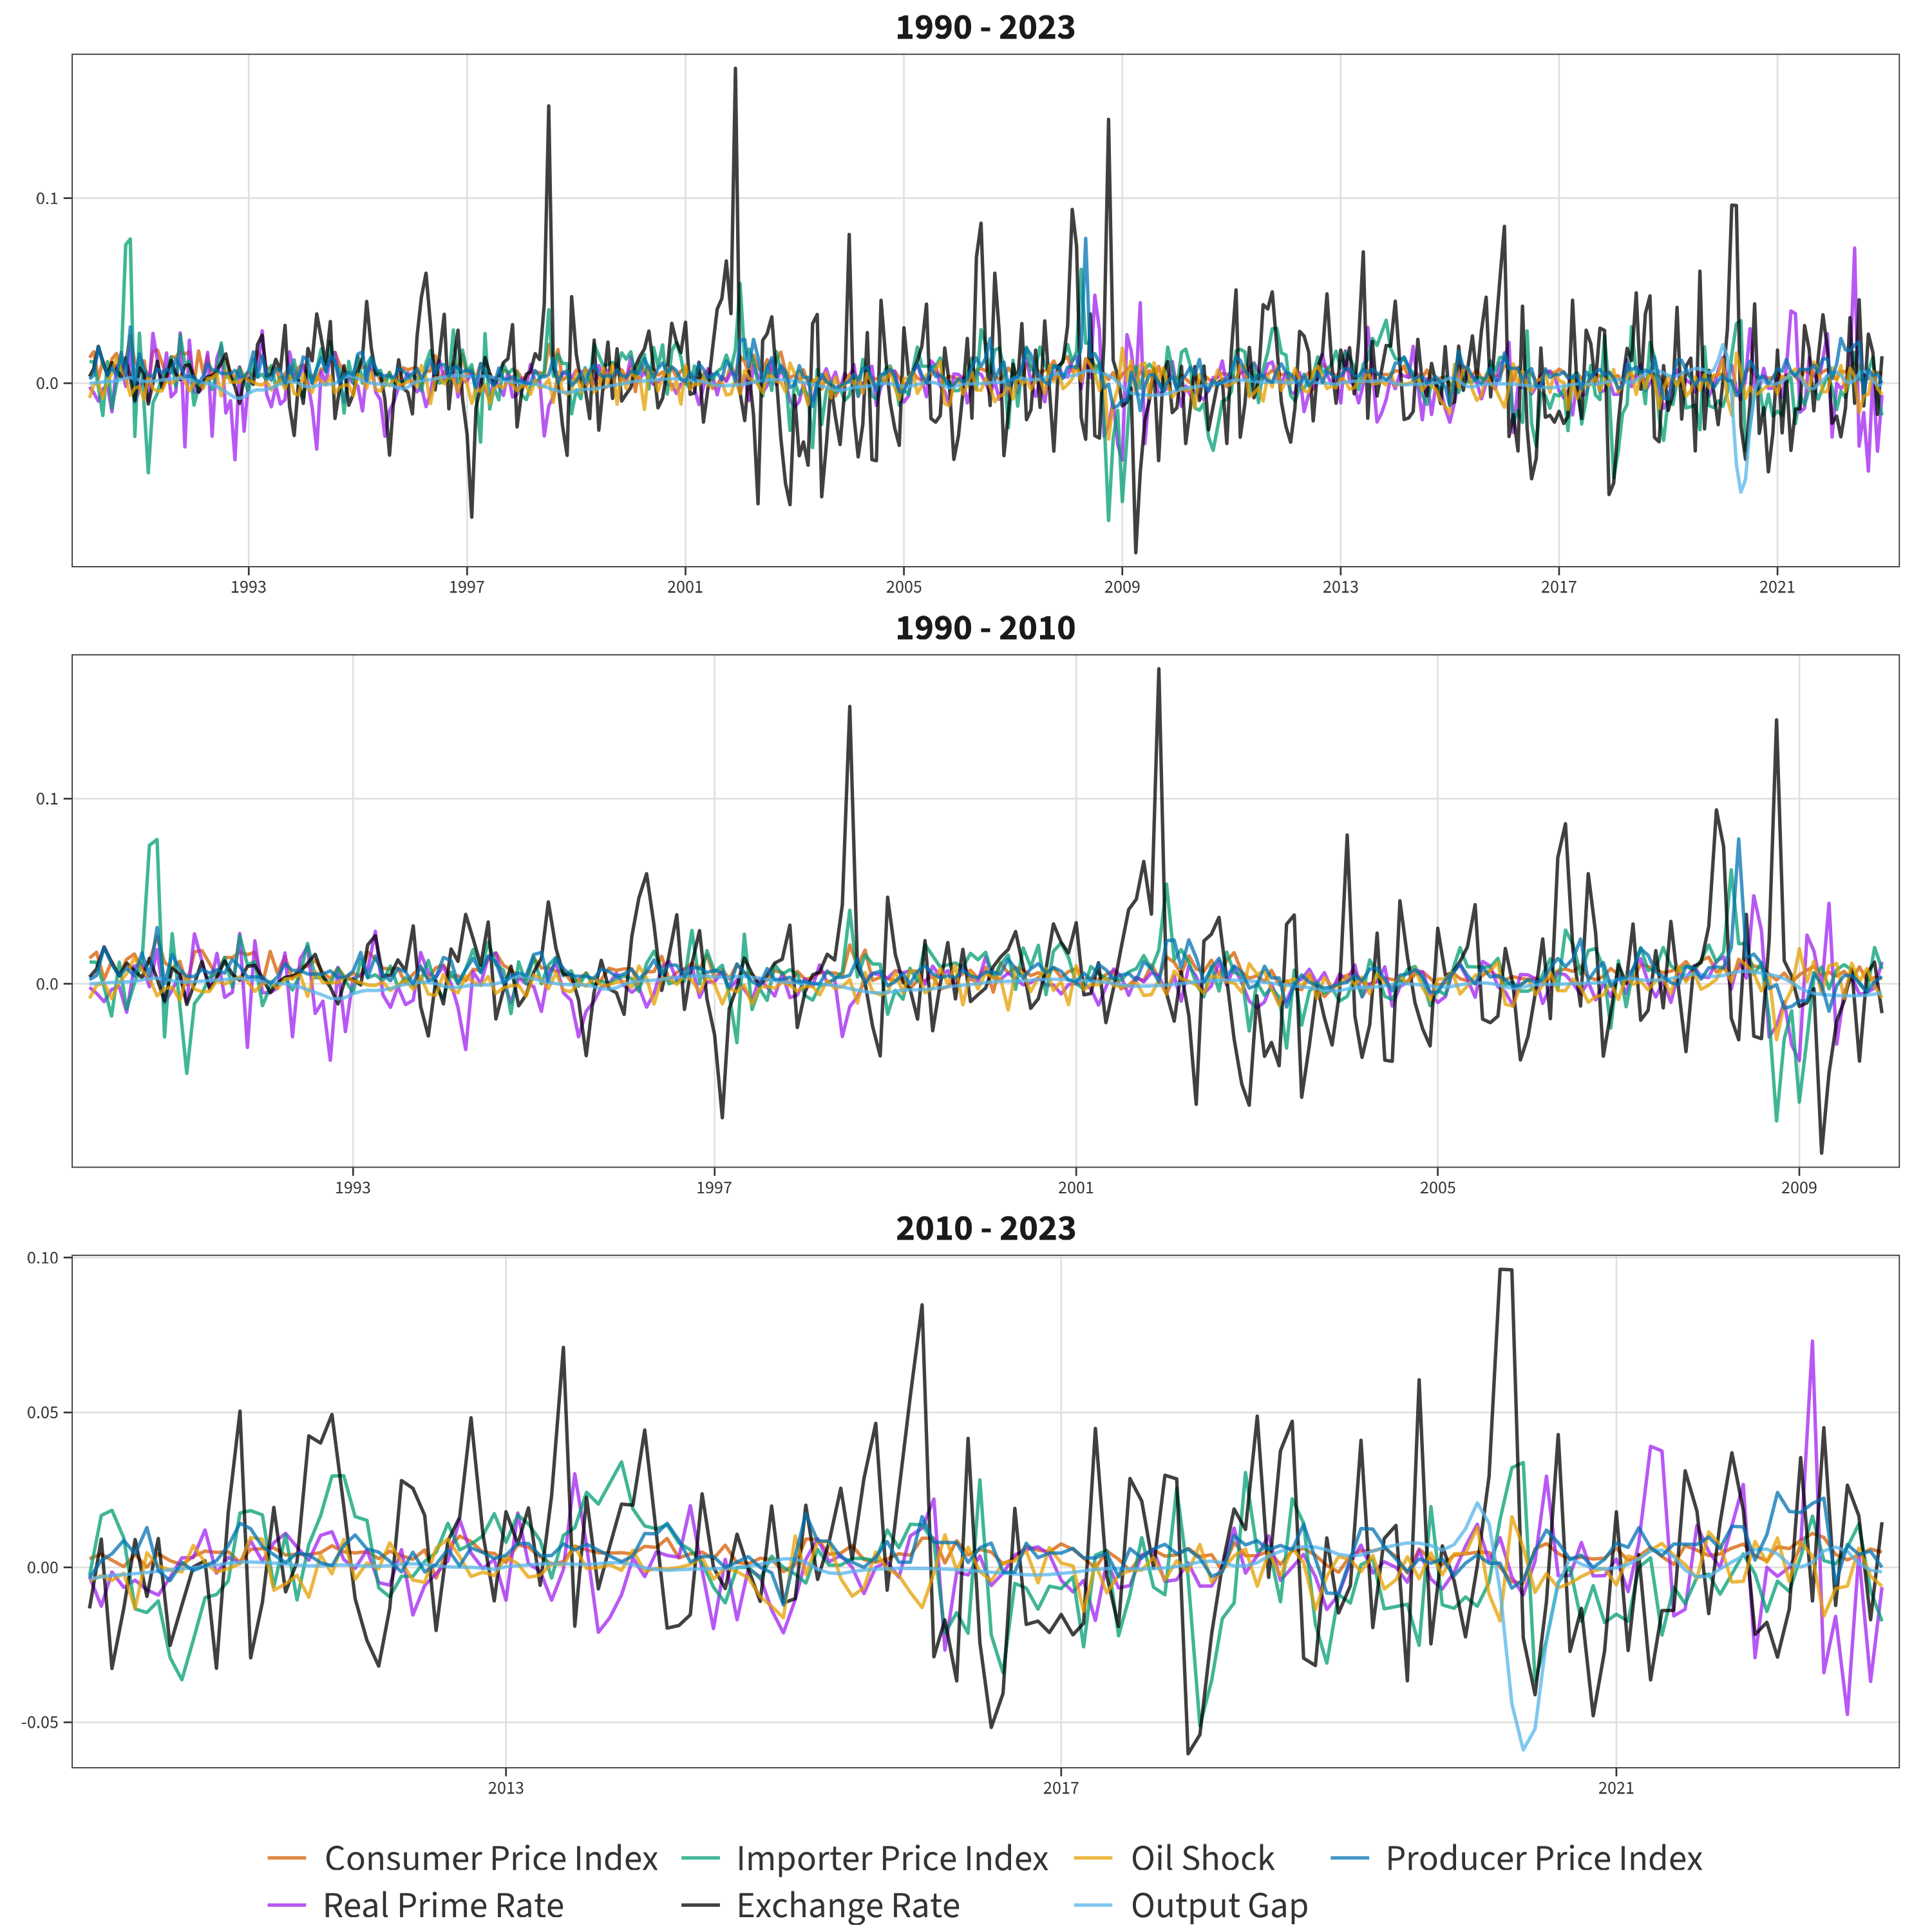
\includegraphics[width=\textwidth]{stationarity_combined.png}
    \caption{Variable Time Series Plots}
    \label{fig:stationarity_plots}
\end{figure}

\input{adf_results.txt}
\begin{minipage}{\linewidth}
\footnotesize
\textit{Note:} ADF test with lag length selected by AIC up to a maximum of 12 lags. H$_0$: series contains a unit root. Rejection at the 5\% level indicated.
\end{minipage}

\subsubsection*{B4 - Normality}

\input{normality.txt}

\subsection*{B5 - Lag Selection}
\input{lag_selection.txt}

\subsection*{B6 - Independence}

\input{residcor.txt}

\begin{figure}[H]
    \centering
    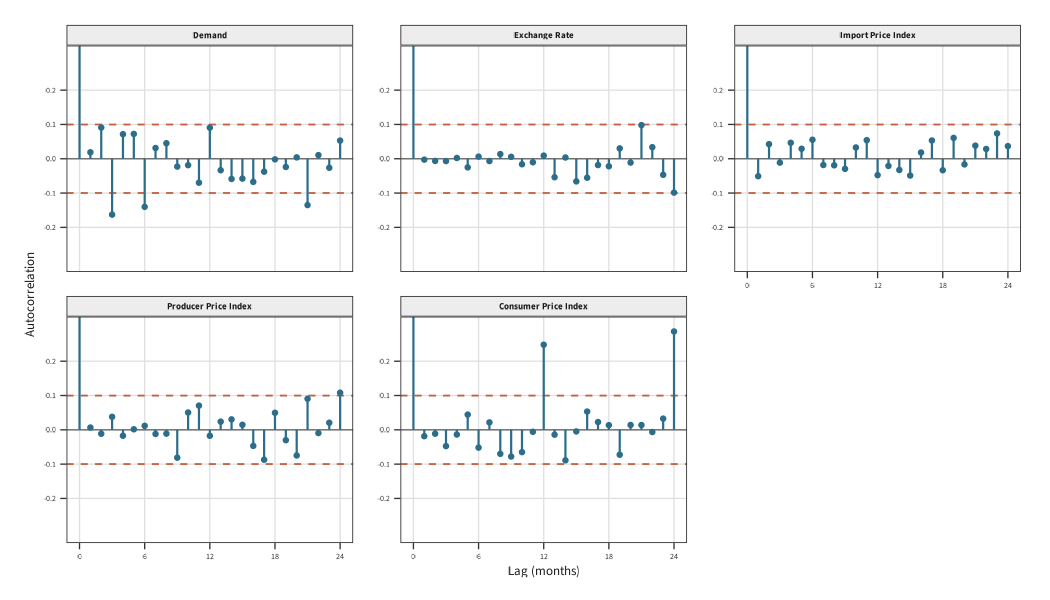
\includegraphics[width=\textwidth]{main_acf.png}
    \caption{Autocorrelation Functions 1990 - 2023}
    \label{fig:acf_plots_full}
\end{figure}


\begin{figure}[H]
    \centering
    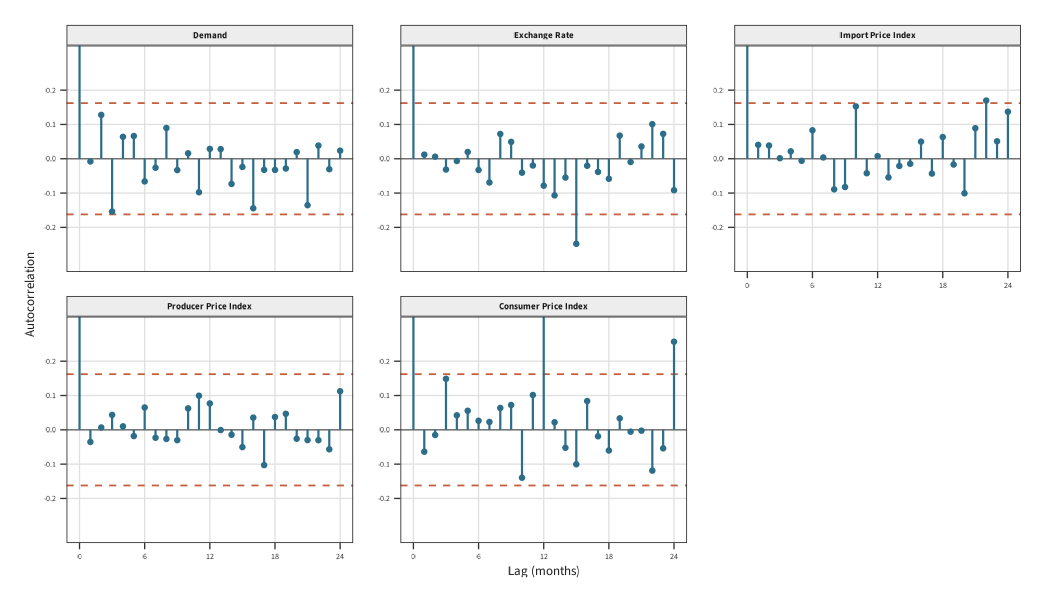
\includegraphics[width=\textwidth]{main_acf_2010.png}
    \caption{Autocorrelation Functions 2010 - 2023}
    \label{fig:acf_plots_2010}
\end{figure}

\begin{figure}[H]
    \centering
    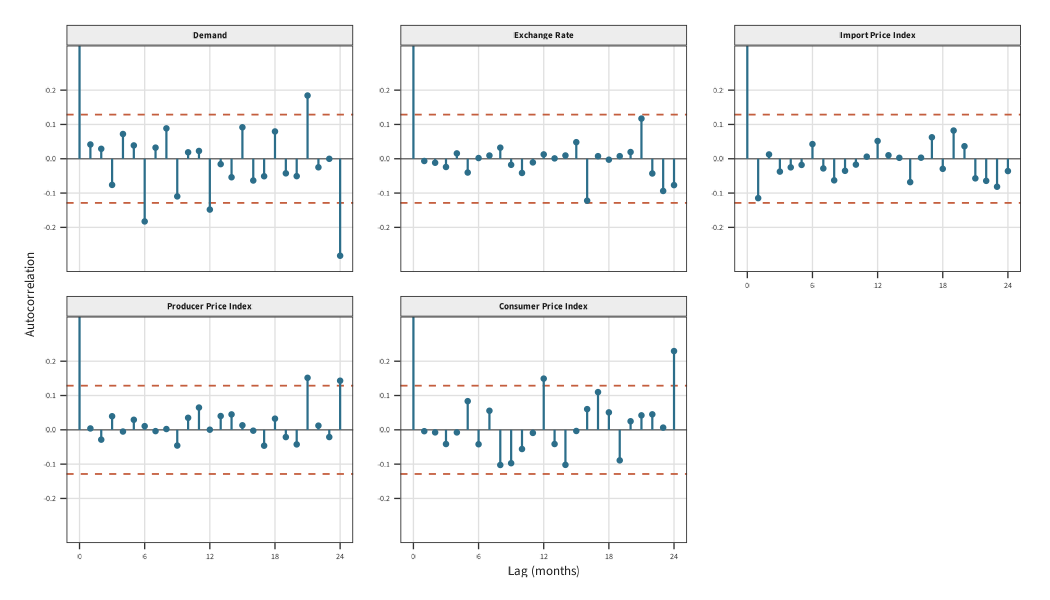
\includegraphics[width=\textwidth]{main_acf_early.png}
    \caption{Autocorrelation Functions 1990 - 2010}
    \label{fig:acf_plots_early}
\end{figure}


\subsection*{B7 - Linking Tests}

\subsubsection*{SIC and UVI (Arithmetic)}

\begin{table}

\caption{Paired t-test: UVI vs SIC import price series}
\centering
\begin{tabular}[t]{rrrrrr}
\toprule
Mean diff. & t & p & CI low & CI high & df\\
\midrule
-0.0028 & -0.9088 & 0.3698 & -0.0092 & 0.0035 & 34\\
\bottomrule
\end{tabular}
\end{table}


\begin{figure}[H]
    \centering
    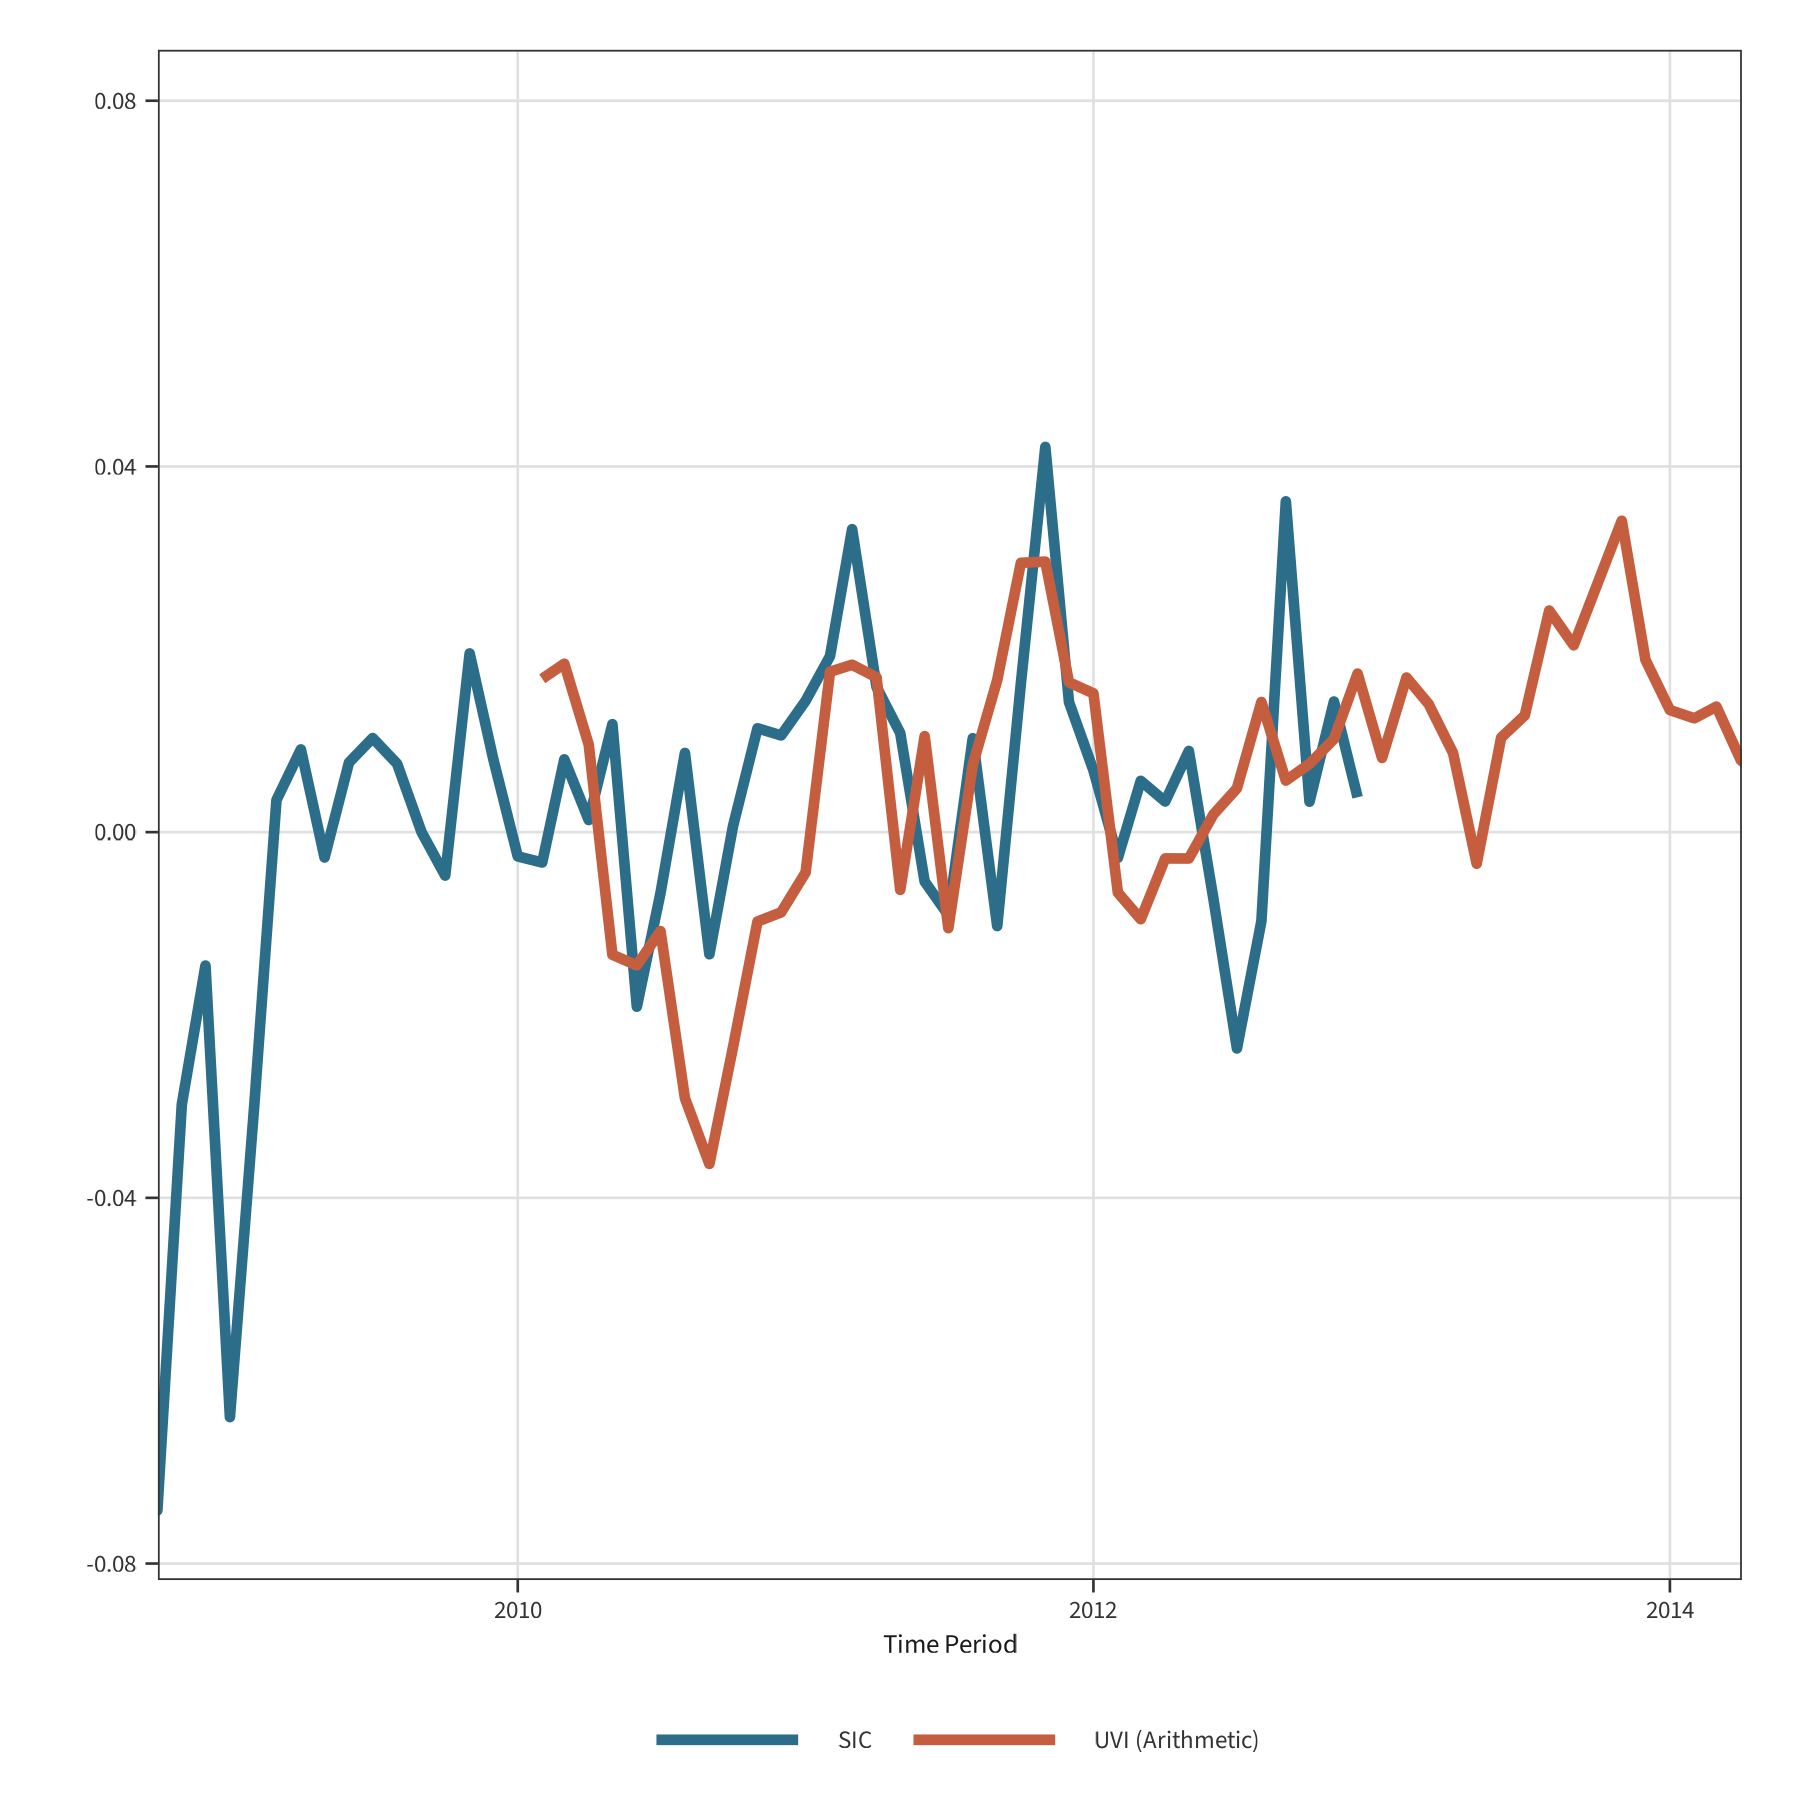
\includegraphics[width=\textwidth]{sic_uvi.png}
    \caption{Overlap period for SIC and UVI (Arithmetic) Indices}
    \label{fig:uvisic_plot}
\end{figure}

\input{chow_test.txt}

\subsubsection*{UVI (Arithmetic) and UVI (Geometric)}


\begin{figure}[H]
    \centering
    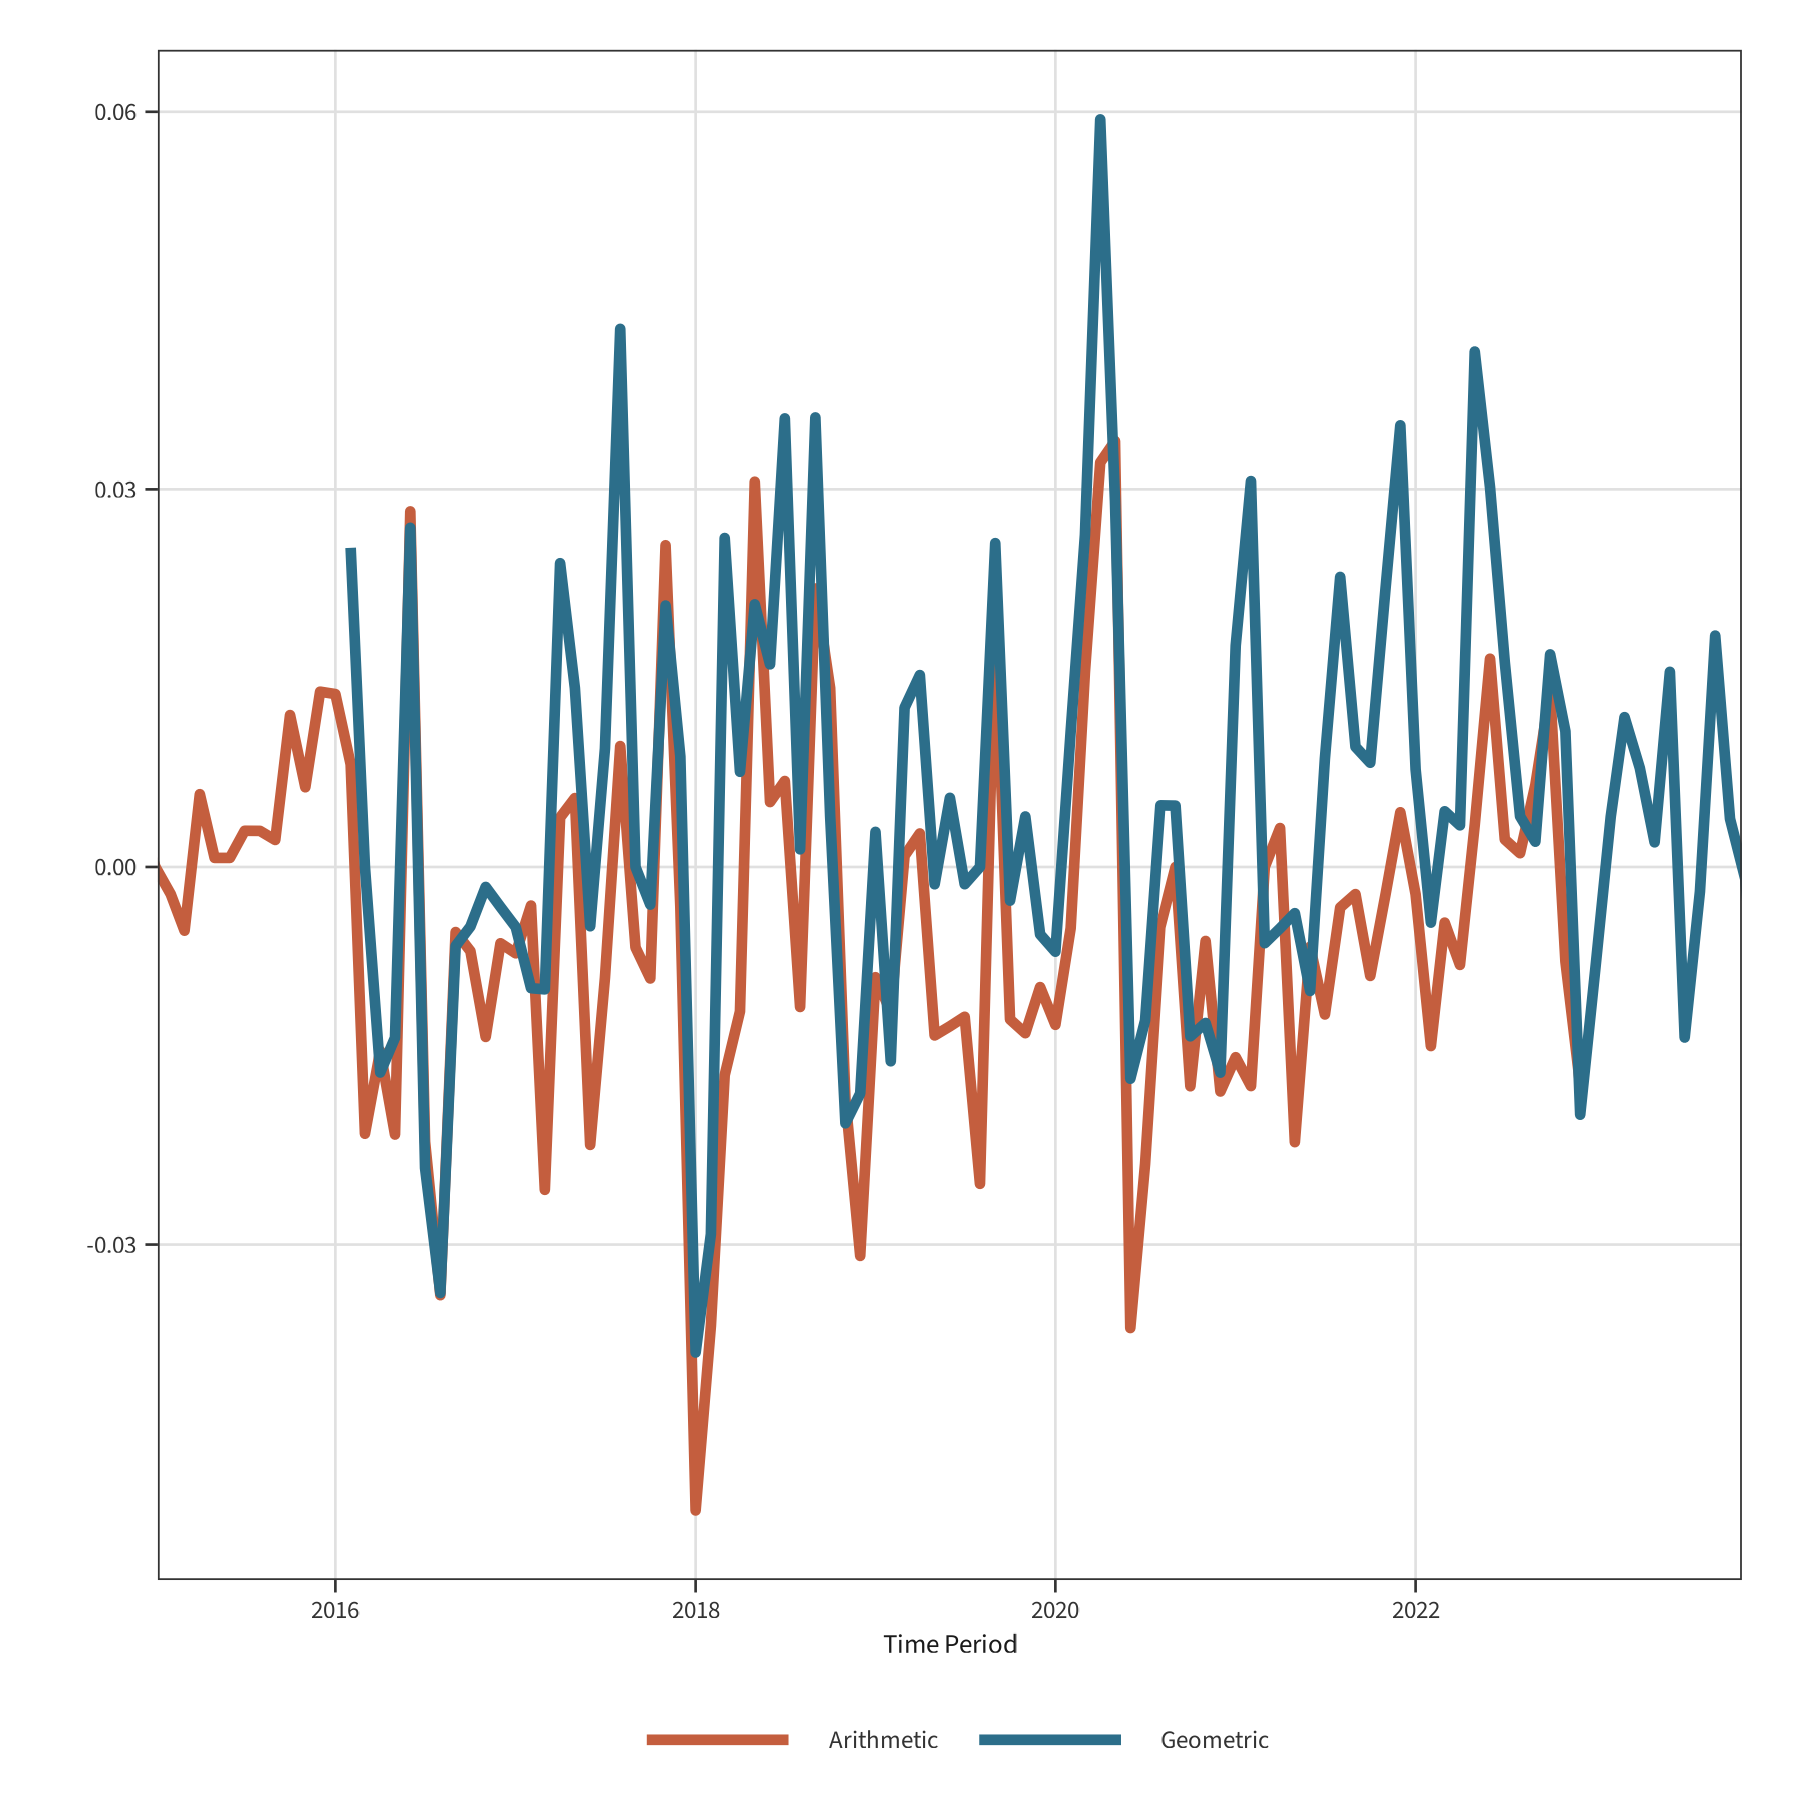
\includegraphics[width=\textwidth]{arit_geom.png}
    \caption{Overlap period for Arithmetic and Geometric UVI Indices}
    \label{fig:aritgeom_plot}
\end{figure}

\begin{table}

\caption{Paired t-test: Arithmetic vs Geometric UVI }
\centering
\begin{tabular}[t]{rrrrrr}
\toprule
Mean diff. & t & p & CI low & CI high & df\\
\midrule
-0.0107 & -8.2249 & 0 & -0.0133 & -0.0081 & 82\\
\bottomrule
\end{tabular}
\end{table}



\newpage
\printbibliography
\end{document}
\bibliography{citations} 